%% Used Compiler: pdfLaTeX / XeLaTeX
%% Diese Arbeit wurde unter Berücksichtigung der Hinweise_Abschlussarbeiten_22.11.2013.pdf, die durch das
%% Institut für Finanzwirtschaft an der TU-Braunschweig bereitgestellt wird, erstellt.

%-------------------------------------------
%% Zusätzliche Pakete werden geladen
%\documentclass[a4paper,12pt,titlepage]{article}  
\documentclass[a4paper, 12pt, titlepage]{scrartcl} % Schrift- und Papiergröße werden eingestellt  
\usepackage[top=3cm, bottom=3cm, left=2.5cm, right=2.5cm]{geometry} % Korrekturrand wird eingestellt
\usepackage[ngerman]{babel}             % Dokumentsprache wird auf deutsch gesetzt
\usepackage[onehalfspacing]{setspace}   % Zeilenabstand wird auf 1,5 gesetzt
\usepackage{color}                      % Ermöglicht die Änderung der Schriftfarbe
\usepackage{graphicx}                   % Ermöglicht das Einbinden von Bildern
\usepackage{fancyhdr}                   % Ermöglicht die freie Bearbeitung der Fuß und Kopfzeilen
\usepackage{tocloft}                    % Ermöglicht das anpassen des Inhaltsverzeichnisses
\usepackage{wrapfig}                    % Ermöglicht textumschlossene Abbildungen
\usepackage{array}                      % Ermöglicht das Anpassen von Tabellen

%-------------------------------------------
%% Fonteinstellungen abhängig vom Compiler
%% Quellen: https://en.wikibooks.org/wiki/LaTeX/Fonts
%%          https://www.sharelatex.com/learn/XeLaTeX
%%          https://tex.stackexchange.com/questions/12565/load-fonts-that-are-in-a-fonts-directory
\usepackage{ifxetex}                    % Ermöglicht das Prüfen ob XeLaTeX benutz wird
    \ifxetex
    \usepackage{fontspec}
    \defaultfontfeatures{Ligatures=TeX} % To support LaTeX quoting style
    \setmainfont[%                      % Times New Roman (aus Windows) wird als Standardschrift gesetzt
        Path = Fonts/,%                 % Dateien Pfad wird auf Fonts/ gesetzt
        BoldFont=timesbd.ttf,%
        ItalicFont=timesi.ttf,%
        BoldItalicFont=timesbi.ttf,%
        ]{times.ttf}
\else
    \usepackage[T1]{fontenc}            % Liefert die meisten Text-Zeichen für westeuropäische Sprachen
    \usepackage[utf8]{inputenc}         % Ermöglicht die direkte Eingabe der Umlaute
    \usepackage{mathptmx}               % Times wird als Standardschrift gesetzt
\fi

%-------------------------------------------
%% Pakete für das Erstellen von Refferenzen
\usepackage{varioref}
\usepackage{hyperref} % Erweitert die Referenzmöglichkeiten
\usepackage{cleveref}

%-------------------------------------------
%% Pakete für das Erstellen des Literaturverzeichnisses
\usepackage[babel,german=quotes]{csquotes}  % Verwendet die deutsche Art der Anführungszeichen
\usepackage[backend=biber, style=authoryear, citestyle=authoryear, maxitems=1]{biblatex}

\DefineBibliographyStrings{german}{%    % Verändert beim zitieren "u.a." zu "et al." und "und" zu "and"
  andothers = {et al.},
  and       = {and}
}
\addbibresource{10_literatur.bib}       % Fügt die Literaturverzeichnisdatei ein
\setlength{\bibitemsep}{10pt}           % Stellt den Zeilenabstand zwischen den Literaturverzeichnis Einträgen ein
%-------------
%% Erstellt ein Makro welches prüft ob die eingegebene Variable leer ist
\def\ifempty#1{% 
\def\temp{#1}%
\ifx\temp\empty%
}
%-------------
%% Erstellt mit \fcite ein Zitat in der Fußzeile in der Form "Vgl. Kramer (2009), S. 2."
\newcommand{\fcite}[2][]{%              
\ifempty{#1}%
\footnote{Vgl.~\citeauthor{#2}~(\citeyear{#2}).}%
\else%
\footnote{Vgl.~\citeauthor{#2}~(\citeyear{#2}),~S.~#1.}%
\fi%
}
%-------------
%% Statt \textcite kann nun auch \citet verwendet werden
\newcommand{\citet}[2][]{%              
    \ifempty{#1}
        \citeauthor{#2}~(\citeyear{#2})
    \else
        \citeauthor{#2}~(\citeyear{#2}),~S.~#1
    \fi
}

%-------------------------------------------
%% Pakete für die richtige Darstellung von Fußnoten
\usepackage[bottom]{footmisc}           % Setzt die Fußnoten ans Ende der Seite
\usepackage{caption}
%\usepackage{savefnmark}
%\footnotesep\baselineskip
%\deffootnote{0.6cm}{1em}{\makebox[0.6cm][l]{\thefootnotemark}}
\setkomafont{footnote}{\fontsize{10pt}{10.5pt}\selectfont}  % Stellt die Fußnotengröße auf 10 ein
\setlength{\footnotesep}{10pt}                              % Sellt den Fußnotenzeilenabstand auf einfachen Zeilenabstand ein

%-------------------------------------------
\usepackage{lipsum}                     % Erstellt blindtext

%-------------------------------------------
%% Deckblatt
\usepackage{pdfpages}                   % Ermöglicht das Einbinden von PDF Dokumenten (wird verwendet für die Einbindung der Aufgabenstellung)
\usepackage[[showboxes,absolute]{textpos}   % Ermöglicht das Setzen von Inhalt an einem beliebigen Ort
\usepackage{tikz}

\newcommand\Mygrid{%                        % Erzeugt ein Grid für textpos mit \Mygrid        
\tikz[
  remember picture,
  overlay,
  yscale=-1,
  xstep=\TPHorizModule,ystep=\TPVertModule,
  yshift=0pt,xshift=0pt]
  \draw (current page.north west) grid (current page.south east);}

%  yshift=13pt,xshift=4pt]
%-------------------------------------------
%\usepackage{amsmath}
%\usepackage{adjustbox}

\setlength{\parindent}{0pt}             % Entfernt den Einzug der ersten Zeile

\pagestyle{fancy}                       % Ermöglicht benutzerdefinierte Kopf- und Fußzeilen
\lhead{}
\chead{}
\rhead{\thepage}                        % Seitenangabe oben rechts
\cfoot{} 
\renewcommand{\headrulewidth}{0pt}      % Breite des Dekostriches in der Kopfzeile
\renewcommand{\footrulewidth}{0pt}      % Breite des Dekostriches in der Fußzeile

\newcommand{\titel}{Modellierung und Prognose von Strompreisen durch Neuronale Netze}   % Erstellt eine Variable mit dem Titel der Arbeit
\newcommand{\abgabedatum}{!!13. April 2018!!}   % Erstellt eine Variable mit dem Abgabedatum der Arbeit
\newcommand{\name}{Dennis Albrecht}     % Erstellt eine Variable mit dem Namen des Verfassers

\newcommand\blankpage{%                 % Ermöglicht die Erstellung leerer Seiten mit \blankpage
    \null
    \thispagestyle{empty}%
    \newpage%
}

\renewcommand{\cftsecleader}{\textbf{\cftdotfill{\cftdotsep}}} % Füllt den Leerraum der Sectionenangaben im Inhaltsverzeichnis mit Punkten bis zur Seitenzahl (standardmäßig bei article-class nur ab subsections)

\newcommand{\farbig}[2][red]{\textcolor{#1}{#2}}      % Ermöglicht text mit \farbig{text} rot einzufärben

%-------------------------------------------
%% Einstellungen für die richtige Nummerierung von Fußnoten und Hyperlinks
%% Quelle: https://tex.stackexchange.com/questions/41626/wrapfigure-footnote-hyperlinks
\makeatletter
\newcommand{\wrapfigfoot}{%
\addtocounter{footnote}{+1}%
\addtocounter{Hfootnote}{+1}%
\global\let\Hy@saved@currentHref\@currentHref%
\hyper@makecurrent{Hfootnote}%
\global\let\Hy@footnote@currentHref\@currentHref%
\global\let\@currentHref\Hy@saved@currentHref%
}
\makeatother
%-------------------------------------------

\begin{document}

%---------------------------------------------------------------------------------
%% Titelseite

%% !TEX root = 00_arbeit.tex

%---------------------------------------------------------------------------------
%% Titelseite
\begin{titlepage}
\thispagestyle{empty}
\begin{doublespace}
\centering

%\Mygrid

\begin{center}
	
\includegraphics[width=1.0\textwidth]{Bilder/Offiziell/TUBSIF.pdf}
\end{center}

\vspace{1cm}

\begin{singlespacing}
    {\small Masterarbeit\\zur Erlangung des akademischen Grades\\Master of Science\\ \vspace{2cm}}
\end{singlespacing}


{\huge \textcolor{red}{\textbf{\titel}}}\\ \vspace{2cm}
{\small Vorgelegt von:\\ \vspace{1cm}}

{\Large B.Sc. \name}\\

\begin{singlespacing}
    albrecht.dennis@live.de\\Wirtschaftsingenieurwesen Elektrotechnik\\Matr.-Nr.: 4603931\\
\end{singlespacing}

\vspace{6cm}


%\abgabedatum\\ \vspace{2cm}
\begin{singlespacing}
    Carl-Friedrich-Gauß Fakultät: Institut für Finanzwirtschaft\\Technische Universität Braunschweig\\Braunschweig, März 2018\\
\end{singlespacing}

\begin{textblock*}{20mm}(25mm,195mm)
\raggedright
    Betreuer:
\end{textblock*}

\begin{textblock*}{80mm}(25mm,200mm)
\raggedright
    Dipl.-Wirtsch.-Ing. Thomas Paulsen
\end{textblock*}



\begin{textblock*}{38mm}(25mm,218mm)
\raggedright
    Erstprüfer:
\end{textblock*}

\begin{textblock*}{38mm}(25mm,223mm)
\raggedright
    Prof. Dr. Marc Gürtler
\end{textblock*}



\begin{textblock*}{48mm}(137mm,218mm)
\raggedright
    Zweitprüfer:
\end{textblock*}

\begin{textblock*}{48mm}(137mm,223mm)
\raggedright
    Prof. Dr. Christian Leßmann
\end{textblock*}


\end{doublespace}
\end{titlepage}
%---------------------------------------------------------------------------------
\blankpage
%---------------------------------------------------------------------------------
%% Aufgabenstellung

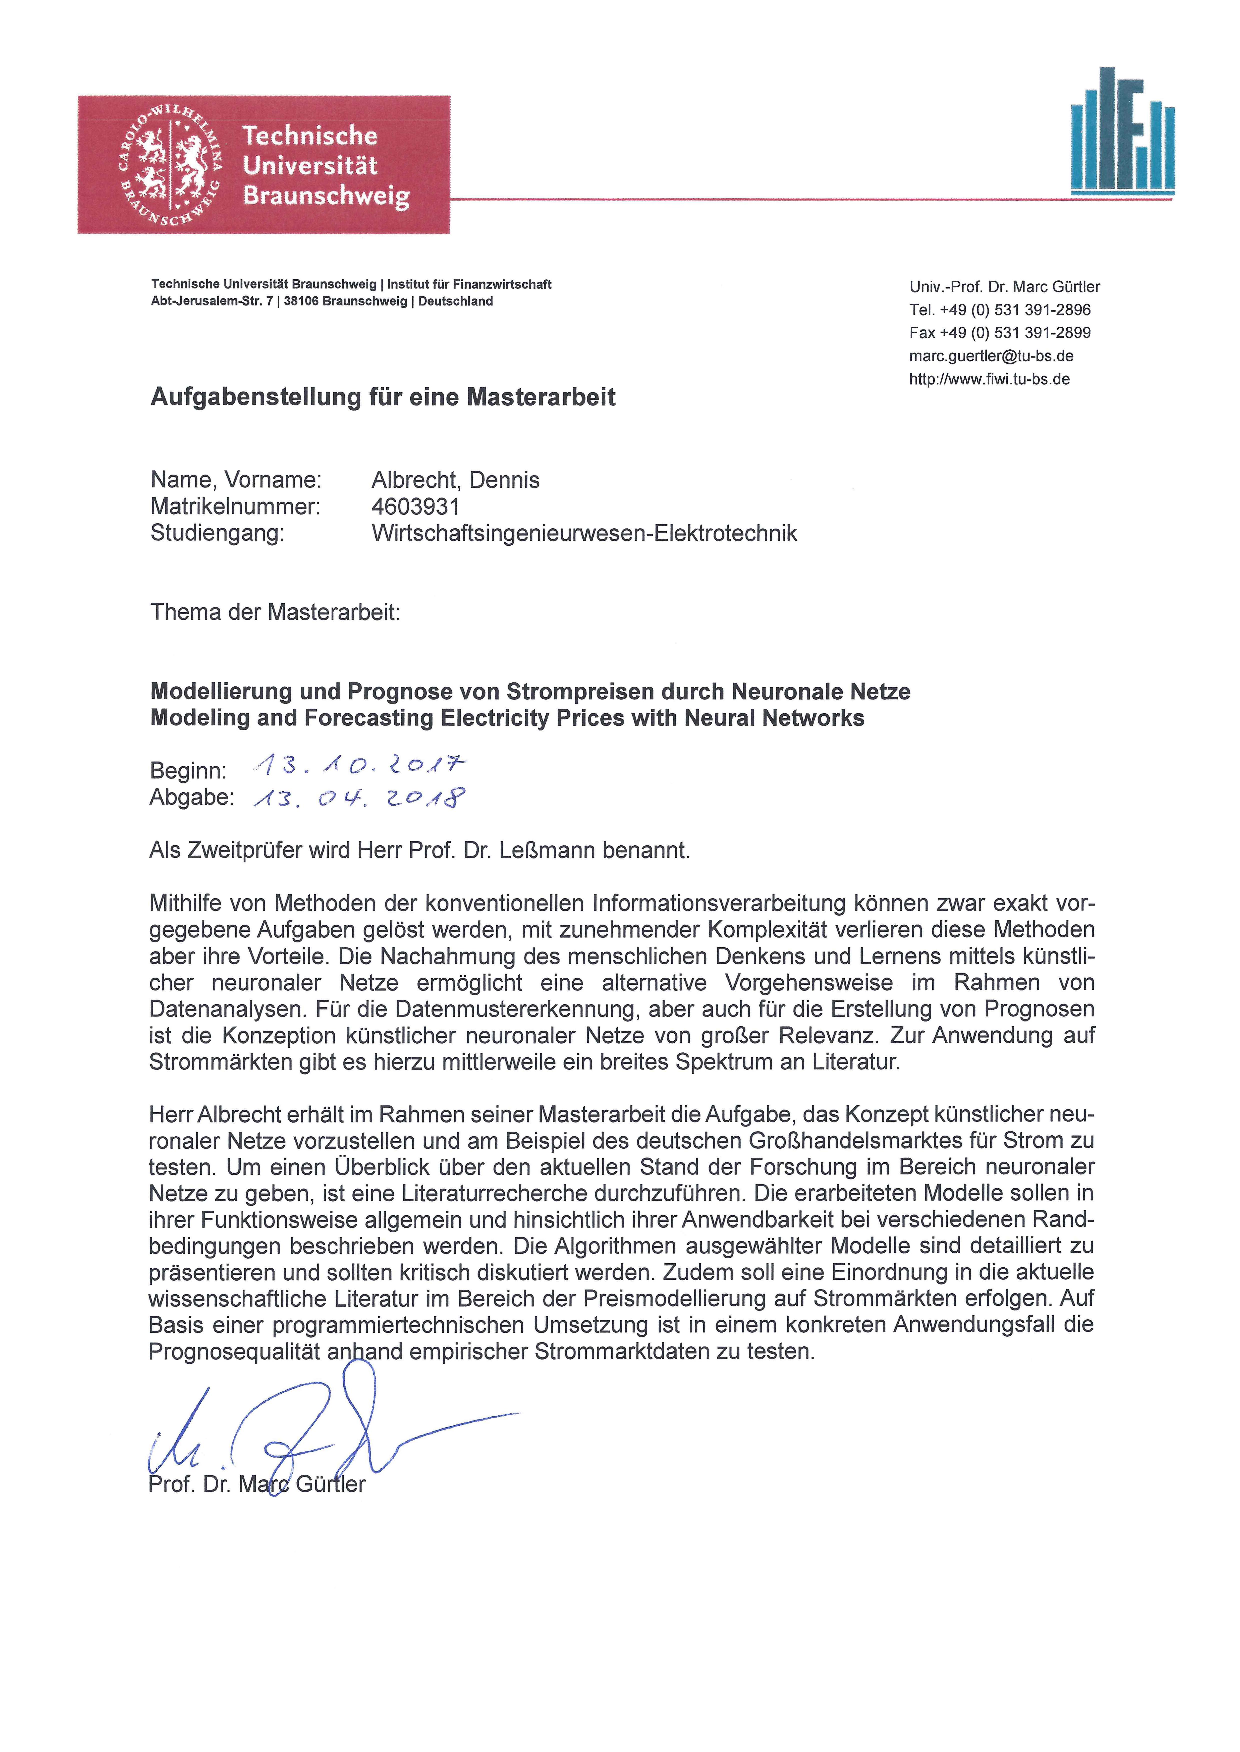
\includepdf[pages=-]{Bilder/Offiziell/Aufgabenstellung_Masterarbeit_600dpi_rot.pdf}    % Fügt alle Seiten des PDF Dokumentes ein

%---------------------------------------------------------------------------------
\newpage
%---------------------------------------------------------------------------------
%% Eidesstattliche Erklärung

%\thispagestyle{empty}
\pagenumbering{Roman}
\setcounter{page}{4}

{\LARGE \textbf{Eidesstattliche Erklärung}}\\ \vspace{1cm}

Ich erkläre hiermit an Eides statt, dass ich die vorliegende  Masterarbeit „\titel“ selbstständig verfasst sowie alle benutzten Quellen und Hilfsmittel vollständig angegeben habe.\\ \vspace{1cm}

Braunschweig, den \abgabedatum\\ \vspace{1cm}

\name
%---------------------------------------------------------------------------------  

%---------------------------------------------------------------------------------
\newpage
%---------------------------------------------------------------------------------
%% Vorlauf

\pagenumbering{Roman}

% !TEX root = 00_arbeit.tex

%---------------------------------------------------------------------------------
%% Inhaltsverzeichniss

\setcounter{page}{5}
{
\setstretch{1.3} 
\tableofcontents%
}
{
\setstretch{1.27} 
\newpage
\printglossary[type=abbreviations, title={Abkürzungsverzeichnis}]%
\newpage
\listoffigures%
\newpage
\listoftables%
\newpage
\printglossary[type=symbols,  nopostdot=false, title={Variablenverzeichnis}]%style=superborder,
}




%---------------------------------------------------------------------------------
\newpage
%---------------------------------------------------------------------------------
%% Hauptteil

\pagenumbering{arabic}

% !TEX root = 00_arbeit.tex

%---------------------------------------------------------------------------------
%% Einleitung

\section{Einleitung}

\blankpage
\blankpage

% Der Theorieteil wird informativ gehalten wobei ausgewählte Algorithmen im nachgang mathematisch vorgestellt werden.
% !TEX root = 00_arbeit.tex

%---------------------------------------------------------------------------------
%% Theorie

\section{Neuronale Netze}
%\farbig{[Erklärung der neuronalen Netze... vielfältige Anwendungsgebiete... Hier erforderlich Netze zur Zeitreihenvorhersage]}
%\setlength{\intextsep}{0pt}%
\begin{wrapfigure}{r}{0.5\textwidth}
    \centering
        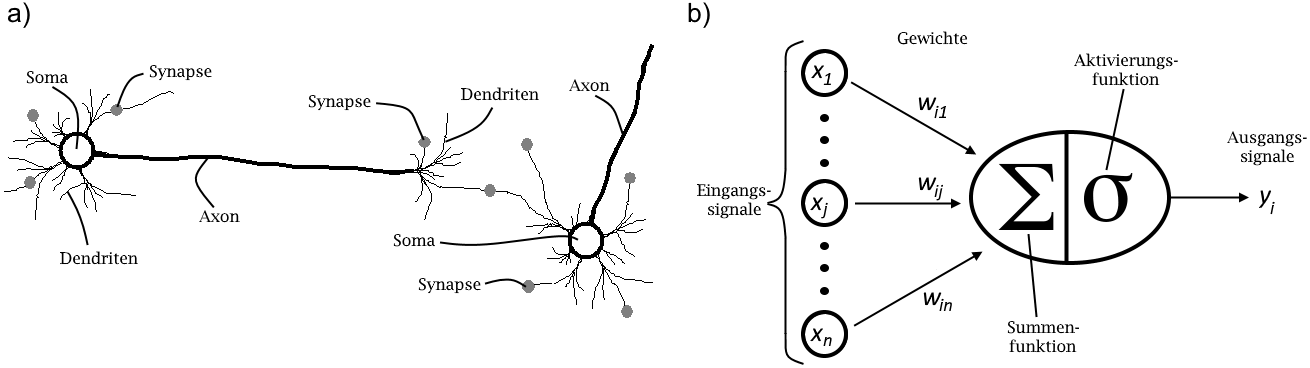
\includegraphics[width=0.5\textwidth]{Bilder/BNN_ANN.png}
    \caption{Gegenüberstellung eines Ausschnittes aus einem biologischen neuronalen Netz a)\protect\footnotemark{} und einem künstlichen neuronalen Netz b).}
    \label{fig:BNN_ANN}
\end{wrapfigure}

\addtocounter{footnote}{-1}%  -1 mal die Gesamtanzahl an Fußnoten in der wrapfigure
\addtocounter{Hfootnote}{-1}% -1 times total number of footnote(mark)s in the wrapfigure
\wrapfigfoot\footnotetext{\autoref{fig:BNN_ANN} a) und \autoref{tab:BNN_ANN} wurden aus\citet[2]{sen_an} übersetzt und angepasst.}
%\citet[\pno~2~ff.]{sen_an}

Ein künstliches neuronales Netz (engl. artificial neural networks)~(NN) ist ein mathematische Konstrukt. Es bildet ein informationsverarbeitendes System welches aus einer Vielzahl einfacher Einheiten den sogenannten Neuronen besteht. Entstanden ist es Anfang der 40er Jahre des letzten Jahrhunderts\fcite[A1.1:1]{Fiesler96} aus der Untersuchung von biologischen Abläufen im Nervensystem von Wirbeltieren, wo Sinneseindrücke des Körpers aufgenommen und mit Hilfe diverser neuronaler Netze verarbeitet werden. 
\autoref{fig:BNN_ANN} zeigt eine Gegenüberstellung eines künstlichen und biologischen Neurons und \autoref{tab:BNN_ANN} die Analogie seiner Bestandteile. Das zurzeit prominenteste künstliche Neuron (die kleinste Einheit im Netzwerk), dargestellt in \hbox{\autoref{fig:BNN_ANN} b)}, wird nach \citet{perceptron_ros58} als Perzeptron bezeichnet. Es summiert zunächst die gewichteten Eingänge mit $\varphi (x)=\sum_{i=1}^{n}x_{i}\omega_{i}$, anschließend wird die gewichtete Summe~$\varphi(x)$ über die Aktivierungsfunktion~$\sigma(x)$ als Ausgang~$y$ an das nächste Neuron übergeben.%

\setlength{\intextsep}{0pt}%
%\setlength{\columnsep}{10pt}%
\begin{wraptable}{l}{6.4cm}
    \caption {Analogie zwischen biologischen und künstlichen Neuronen.}
    \begin{tabular}{>{\centering\arraybackslash}m{2.2cm}>{\centering\arraybackslash}m{3.4cm}}
    \hline
    Biologisches\newline Neuron & Künstliches\newline Neuron            \\ \hline \hline
    Soma                & Summen- und\newline Aktivierungsfunktion      \\ 
    Dendrit             & Eingang                                       \\ 
    Axon                & Ausgang                                       \\ 
    Synapse             & Gewicht                                       \\ \hline
    \end{tabular}
    \label{tab:BNN_ANN}
\end{wraptable}

Klassische Aktivierungsfunktionen sind dabei die \hbox{Heaviside-,} die lineare Schwellwert-, die Fermifunktion und der Tangens Hyperbolicus\footnote{Vgl. \citet[5]{neuralnet_intro} und \citet[39 f]{dkriesel07}.}.\\

Es gibt Problemstellungen die mit klassischen mathematischen Modellen und Algorithmen gar nicht oder nur schwer zu lösen sind. Neuronale Netze unterscheiden sich zu klassischen Algorithmen durch ihre Lernfähigkeit. Ohne explizite Programmierung sind sie in der Lage eine Aufgabe anhand von Trainingsbeispielen zu erlernen. Einige Beispiele wären die Gesichtserkennung oder die Erkennung von menschlicher Sprache.
\newpage

Künstliche neuronale Netze sind augenblicklich eine Disziplin der Computional Intelligence~(CI), welches wiederum einen Teilbereich der Künstlichenintelligenz (artificial intelligence)~(AI) darstellt. Diese fasst verschiedene von der Natur inspirierte Berechnungsmethoden zusammen. Weitere Methoden der CI sind Fuzzy-Systeme~(FS), Evolutionäre Algorithmen~(EA), Schwarmintelligenz~(SI) und Künstliche Immunsysteme~(AIS).\fcite[11 ff]{Kroll16} Obwohl sich diese Arbeit wesentlich mit NN beschäftigen wird, wird an dieser Stelle auf weitere CI-Methoden hingewiesen, da in der Literatur hybride CI-Systeme bekannt sind und auch genutzt werden.

\subsection{Charakterisierung und Anwendung künstlicher neuronaler Netze}

Da es nicht das NN gibt sondern viele unterschiedliche Arten, die teilweise spezielle Anwendungsgebiete finden, werden in diesem Unterkapitel Charakterisierungskriterien für NN vorgestellt. Schließlich wird ein Überblick über mögliche Anwendungsgebiete gegeben.\\

Im allgemeinen können NN anhand der folgenden drei Kriterien charakterisiert werden\fcite[7 ff]{characterisation_4}:%

\begin{enumerate}
\item%
Nach der Art des verwendeten Neurons.\\
Dazu gibt es in der Literatur vielfältige Beispiele. \citet{Fiesler96} zählen einige Beispiele im Kapitel B1 auf und weisen auf Unterschiede hin. Als Beispiel wird dort das bereits erwähnte Perceptron beschrieben. Dann gehen sie auf das Neuron des Hopfield-Netzwerkes ein, bei dem das Neuron ein Teilchen beschreibt welches sich in einem Magnetfeld ausrichtet. Ein eher exotischer Vertreter der dort nicht erwähnt wird ist das Fuzzy-Neuron von \citet{fuzzy-neuron}, welches nach der Aktivierung mehrere mögliche Zustände einnehmen kann und seine Anwendung in der Mustererkennug findet.

\item%
Nach der Topologie buw. der Verbindungsarchitektur.\\
Sie beschreibt wie Neuronen in einem Netzwerk verbunden sind.
Es werden folgende Architekturen unterschieden:
\begin{itemize}
\item[\textbf{$\bullet$}]%
Autoassoziative: Hierbei fungieren die Eingangs- gleichzeitig als Ausgangsneurone (z.B. das Hopfield-Netzwerk). 

\item[\textbf{$\bullet$}]%
Heteroassoziative: Unterschiedliche Neurone übernehmen die Rolle der Eingangs- bzw. Ausgangsneurone. Hierzu zählen die Multylayer-Perzeptrons (MLP) bei dem mehrere Schichten von mehrzahligen Perzeptronen ein Netzwerk Bilden\fcite[86 ff]{dkriesel07}. Aber auch das Kohonen Netzwerk auch bekannt als Self Organizing Maps (SOM) bei dem die Neuronen sich selbständig anordnen und der Zustand des Netzes als Ausgabe dient\fcite[153 ff]{dkriesel07}.

Zusätzlich wird unterschieden wie die Verbindungen unter den einzelnen Neuronen realisiert sind. Hier wird zwischen zwei Arten unterschieden:

\item[$\circ$]%
Feedforward: Diese Netzwerke bestehen meistens aus Schichten und eine Schicht ist nur mit der jeweils nächsten Schicht verbunden.

\item[$\circ$]%
Recurrent (Feedback): In der deutschsprachigen Literatur als rückgekoppelte oder rekurrente Netze bezeichnet beeinflussen sich diese Netzwerke selbst. Die Neuronen dieser Netzwerke besitzen eine Verbindung entweder zu sich selbst (direkte Rückkoppelung), zu den Neuronen der vorhergehenden Schicht (indirekte Rückkopplung), zu den Neuronen der gleichen Schicht (laterale Rückkopplung) oder vollständig verbundene Netze (Verbindungen zwischen allen Neuronen ausgenommen der direkten Rückkopplung). Durch die Rückkopplung besitzen diese Netzwerke ein "Gedächtnis"~da der vorherige Zustand in die Auswertung der aktuellen Eingangsinformation mit einfließt.\fcite[42 ff]{dkriesel07} Ein Beispiel für ein vollständig verbundenes Netzwerk ist das Hopfield-Netzwerk.

\end{itemize}

\item%
Nach dem Lernalgorithmus. Dieser ermöglicht es das Netzwerk zu trainieren. Die heutzutage benutzten Algorithmen werden in drei Gruppen unterteilt\footnote{Vgl. \citet[55]{dkriesel07}.\label{kriesel55}}:

\begin{itemize}
\item[\textbf{$\bullet$}]%
Supervised learning (überwachtes Lernen): Die Trainingsbeispiele bestehen aus einer Menge an Eingangsinformationen und den dazugehörigen Ausbangsinformationen. Das Ziel ist es die Differenz zwischen der tatsächlichen Ausgabe des Netzwerks und den vorliegenden Ausgangsinformationen zu minimieren.

\item[\textbf{$\bullet$}]%
Reinforcement learning (bestärkendes Lernen): Plakativ kann diese Lernmethode als Zuckerbrot und Peitsche bezeichnet werden bzw. lernen durch Belohnung und Bestrafung. Hierbei werden die Eingangsinformationen zur Verfügung gestellt und die Ausgabe des Netzwerkes wird anhand einer Belohnungsfunktion bewertet. Wird die Ausgabe als gut/schlecht angesehen so werden die zugehörigen Verbindungen gestärkt/geschwächt\footnote{Vgl. \citet[201]{dkriesel07} und \citet[A2.3:5]{Fiesler96}.}. 

\item[\textbf{$\bullet$}]%
Unsupervised learning (unüberwachtes Lernen): Wird auch als selbstorganisiertes (self organized) Lernen bezeichnet. Die Trainingsbeispiele bestehen hierbei nur aus Eingansinformationen. Das Netzwerk versucht aus den Eingansinformationen selbstständig Ähnlichkeiten zu erkennen.
Unüberwachte Lernmethoden werden noch unterteilt in konkurrierendes (competitive) und nicht konkurrierendes (noncompetitive) Lernverfahren. Der unterschied besteht darin dass bei dem konkurrierenden Verfahren in einem Netzwerk einzelne Gruppen von Neuronen um die Aktivität konkurrieren\fcite[B3.3:5]{Fiesler96}.

Zusätzlich unterscheidet man unter allen drei Lernmethoden zwei Lernarten\fcite[A2.3:3]{Fiesler96}: 
\item[$\circ$]%
off-line learning: Auch Batch-Trainingsverfahren genannt. Hierbei wird die Netzwerkausgabe nach einer Menge von Eingangsinformationnen ausgewertet und anschließend werden die Gewichte angepasst.

\item[$\circ$]%
on-line learning: Hier werden die Gewichte nach jeder einzelnen Beobachtung der gesamten Eingangsinformationen angepasst. 

\end{itemize}

\end{enumerate}

Vollständigkeitshalber wird erwähnt dass \citet{characterisation_4} vier Charakterisierungskriterien nennen. Wobei als viertes Kriterium der Informationsgewinnungsalgorithmus (recall algorithm) aufgeführt ist. In dieser Arbeit wird auf dieses Kriterium verzichtet, da weder \citet{characterisation_4} Einteilung/Auflistung aufführen noch in anderer Literatur dieses Kriterium eine Erwähnung findet.\\

Es gibt vielfältige Anwendungsgebiete für NN. Angefangen bei Optimierungsproblemen, wo das Ziel es ist optimale Werte für ein gegebenes System zu finden. Über die Datenverarbeiteung, wo Bild- bzw. Sprachinformationen verarbeitet, generiert oder komprimiert werden sollen. Bis zur Klassifikation/Erkennung von Mustern, wo es darum geht aus einer Dantemenge zusammenhängende Muster zu erkennen. Weitere Anwendungen sind die Kontrelle/Regelung von industriellen Anlagen und die wichtigste (bezogen auf diese Arbeit) ist die Funktionsapproximation bzw. Zeitreihenmodellierung, wo die Beziehung aus Eingangsinformationen und dem gewünschtem Ausgang zu finden gilt. Dies sind einige kurz umrissene Anwendungsbeispiele. In der Literatur werden deutlich mehr aufgeführt.\footnote{Vgl. \citet[224]{Kroll16}, \citet[15]{comp_int_07} und \citet[F1 ff]{Fiesler96}.}\\

%\farbig{NN sind Black-Box und Analyse ist schwer aber es gibt in der Literatur mögliche Analyseverfahren.}


\subsection{Gängige Modelle}

\subsubsection{Multilayerperzeptrons (MLP)}

\subsubsection{Radiale Basisfunktionen (RBF)}

\subsubsection{Self Organizing Maps (SOM)}

\subsubsection{Hopfield-Netzwerk}


%\lipsum


%\subsection{Multilayerperzeptrons (MLP)}

%\subsection{Radiale Basisfunktionen (RBF)}

%\subsection{Gegenüberstellung von MLP- und RBF-Netzen}
% !TEX root = 00_arbeit.tex

%---------------------------------------------------------------------------------
%% Literaturrecherche

\section{Preisprognose auf Strommärkten}\label{sec:strompreis}

Im vorherigen Abschnitt wurden verschiedene Arten neuronaler Netze vorgestellt. In diesem Abschnitt werden zunächst die Eigenheiten des Strommarktes und die Möglichkeiten der Vorhersage des Strompreises vorgestellt. Es folgt ein Literaturüberblick über die Anwendung künstlicher neuronaler Netze zur Strompreisvorhersage. Abschließend werden die bei der Vorhersage eingesetzten Performancemaße diskutiert.

%\todo{Kapitel einleiten}

\subsection{Der Strommarkt und seine Vorhersagemodelle}\label{sec:vorhersagemodelle}

Elektrizität ist ein besonderes Gut, dessen Erzeugung und Verbrauch gleichzeitig erfolgt. Die Erzeugung dieses Gutes kann kontrolliert werden, wobei sich das Speichern von Elektrizität in einem industriellen Maßstab als schwierig gestaltet. Daher beeinflusst die Nachfrage maßgeblich die zu generierende Menge. Aus diesem Grund verläuft der Handel, im Gegensatz zu anderen Finanz- oder Gütermärkten, oft auf dem sogenannten „Day-ahead“-Markt. Der Strom wird dabei für jede Stunde des nächsten Tages ge- und verkauft. Diese Handelsweise ist für die Marktakteure notwendig, um die Produktions- und Abnahmekapazitäten einander anzupassen. Auf den meisten Märkten müssen die Marktakteure bis zu einer bestimmten Frist ihre 24 Gebote abgeben. Nach Ablauf der Frist erstellt der Marktbetereiber unter Berücksichtigung aller Gebote den Gleichgewichtspreis (engl.: market clearing price) für jede der 24 Stunden. Produzenten, deren Gebot niedriger bzw. Konsumenten, deren Gebot höher oder gleich dem Gleichgewichtspreis ist, bekommen den Zuschlag.\,\citef[7]{Weron2014} Um den Gleichgewichtspreis des nächsten Tages vorherzusagen und ein Gebot möglichst nah am Gleichgewichtspreis abzugeben, gibt es vielfältige Ansätze.

Einen guten Überblick über vorgeschlagene Modelle zur Strompreisvorhersage geben \citet{Aggarwal2009}, \citet{Cerjan2013}, \citet{Weron2014} und \citet{Panapakidis2016} in ihren Reviews. Zunächst können die in \autoref{fig:ann_vorhers._modelle} dargestellten Modelle in einen lang-/mittelfristigen und kurzfristigen Vorhersagehorizont eingeteilt werden. 

\begin{figure}[!htb]
    \centering
        \includegraphics[page=2,width=1\textwidth]{Bilder/misc/ANN_Organigramme.pdf}
    \caption[Modelle die zur Vorhersage des Strompreises]{Organigramm der Modelle die zur Vorhersage des Strompreises eingesetzt werden.\,\protect\footnotemark{}}
    \label{fig:ann_vorhers._modelle}
\end{figure}
\addtocounter{footnote}{-1}     % -1 mal die Gesamtanzahl an Fußnoten in der wrapfigure
\addtocounter{Hfootnote}{-1}    % -1 times total number of footnote(mark)s in the wrapfigure
\wrapfigfoot\footnotetext{\autoref{fig:ann_vorhers._modelle} wurde in Anlehnung an \citet[12]{Weron2014} erstellt.}



Zu dem lang- und mittelfristigen Vorhersagehorizont kommen folgende Modelle zur Anwendung:
\begin{itemize}
\item[\textbf{$\bullet$}]%
Multi-Agenten bzw. Spieltheorie Modelle, bei denen versucht wird, das Verhalten der unterschiedlichen Agenten/Akteure auf dem Markt zu simulieren.

\item[\textbf{$\bullet$}]%
Fundamentale Modelle, bei denen physikalische Faktoren in Zusammenhang mit der Preisdynamik gesetzt werden.

\item[\textbf{$\bullet$}]%
Reduzierte Modelle, welche die statistischen Eigenschaften des zeitlichen Preisverlaufes mit Hilfe der Auswertung von Risiken und Derivaten erklären.
\end{itemize}

Für den kurzfristigen Vorhersagehorizont werden die nachfolgenden Modelle angewandt:
%Zusammenfassend lassen sich die Modelle in folgende Kategorien einteilen:
%\citet{Weron2014} hat die vorgeschlagenen Modelle zur Preisvorhersage in in fünf Kategorien eingeteilt:\footnote{In der Literatur vorkommende Modelle sind oftmals hybride Lösungen, die aus mehreren der genannten Kategorien bestehen.}
\begin{itemize}
\item[\textbf{$\bullet$}]%
Statistische Modelle, welche aus linearer Regression von Zeitreihen und ökonometrischen Modellen bestehen.

\item[\textbf{$\bullet$}]%
Computerbasierte/künstliche Intelligenz (CI), die in Verbindung mit Lern-, Evolutions- und Fuzzyalgorithmen komplexe dynamische Systeme abbilden kann.
\end{itemize}

Die Modelle computerbasierte/künstliche Intelligenz weiter unterteilt werden in: 
\begin{itemize}
\item[\textbf{$\bullet$}]%
Künstliche neuronale Netze

\item[\textbf{$\bullet$}]%
Data-Mining-Modelle
\end{itemize}

%\todo{Der Unterschied zwischen künstlichen neuronalen Netzen und Data-Mining + Modelle nennen }

Die passende Methode zur Strompreisvorhersage hängt von einer Vielzahl von Überlegungen ab. Der Frage, welche Methode die beste ist, um Vorhersagen zu treffen, geht \citet{Chatfield1988} in seiner Arbeit nach. Vor diesem Hintergrund spricht er sechs Empfehlungen aus. Unter anderem ist die Komplexität eines Modells kein Garant für bessere Vorhersagen im Vergleich zu weniger komplexen Modellen. Weiterhin kann die Anzahl an vergangenen Beobachtungen und der gewünschte Vorhersagehorizont eine Orientierung bei der Wahl des passenden Modells geben.
Bei ihren Untersuchungen stellen \citet{Nogales2002} fest, dass in den meisten kompetitiven Strommärkten die Zeitreihen der Strompreise eine hohe Schwankung aufweisen (gleichzusetzen mit hoher Volatilität), mehrere Saisonalitäten besitzen (das heißt, dass die Zeitreihen tages- und wochenabhängigen Peridiozitäten unterliegen ), einen Kalender-Effekt besitzen (Abhängigkeiten von Wochenenden und Feiertagen) und einen hohen prozentualen Anteil an ungewöhnlichen Preisverläufen besitzen. \citet{Vijayalakshmi2015} kommen bei ihrem Review von NN-Implementierungen für die Strompreisprognose zu dem Schluss, dass sich Strompreise, die durch Volatilität, Saisonalität, Preis-Spitzen, Sprünge und Nichtlinearitäten gekennzeichnet sind, oft nur schwer mit ökonometrischen Modellen vorhersagen lassen. NN-basierte Modelle können aber eine mögliche Antwort auf die kurzfristige Strompreisprognose sein. \citet{Weron2014} kommt zu dem Schluss, dass die Stärke der computerbasierten Intelligenz in der Fähihgkeit liegt, mit Komplexität und Nichtlinearität umgehen zu können. \citet{Gareta2006} sind jedoch der Meinung, dass Ergebnisse der NN-Modelle abhängig von der Menge der Eingabedaten sind und dass das Modell einer Überprüfung bedarf.

Die Anzahl und Einteilung der Modelle in unterschiedliche Vorhersagehorizonte weist darauf hin, dass nicht ein Modell allein alle Faktoren erfasst, die zum schließlichen Preis führen. Aus diesem Grund werden in der Literatur hybride Modelle eingesetzt, die aus einigen der genannten Kategorien zusammengesetzt sind. \citet{Cerjan2013} begründen die Benutzung hybrider Modelle damit, dass die einzelnen Modelle unterschiedliche Muster in den Daten erfassen können. Die einzelnen Modelle ermöglichen damit eine Verringerung der Vorhersageabweichungen und verhelfen den Marktakteuren zu dem erhofften Zuschlag.


\subsection{Literaturüberblick über Anwendung künstlicher neuronaler Netze zur Strompreisvorhersage}\label{sec:literaturueberblick}

\citet{Aggarwal2009} und \citet{Panapakidis2016} haben eine tabellarische Übersicht über die bis dato genutzten NN basierten Modelle zur Vorhersage des Elektrizitätspreises vorgestellt. In Anlehnung der beiden Veröffentlichungen erfolgt ein Literaturüberblick von Anfang 2016 bis Ende 2017. 
Vorhersagemodelle basierend auf~NN, die in dieser Zeit veröffentlicht und dem Autor dieser Arbeit zur Verfügung standen, sind in \autoref{tab:ann_lit} dargestellt. Neben den Verweisen sind die eingesetzten Netzwerke, die untersuchten Märkte und das zur Evaluation eingesetzte Performancemaß aufgeführt. In der genannten Literatur kommen zum Teil hybride Modelle vor. Da es der Fokus dieser Arbeit ist einen Überblick über die Anwendung neuronaler Netze zur Strompreisvorhersage zu geben, wurde in der Tabelle nur das zur Anwendung kommende neuronale Netz aufgeführt. 

%\todo{Übersicht über die Märkte und Performancemaße im Anhang erstellen und im Text auf sie Verweisen}

In der betrachteten Zeitperiode werden in der Literatur zur Vorhersage von Strompreisen die verwendeten Netzwerkmodelle als Artificial Neural Network (ANN) bei \citet{Mirakyan2017}, \citet{Gao2017} und \citet{Sandhu2016} aufgeführt, wobei \citet{Davo2016} und \citet{Domanski2017} den allgemeinen Begriff neural Network (NN) nutzen. Weitere Begriffe sind Backpropagation neural Network (BPNN) bei \citet{Wang2017}, Feed-Forward neural Networks bei \citet{Keles2016} oder die Kombination aus beiden Feed-Forward Backpropagation neural Network (FFBPNN) bei \citet{Peter2016}. Zuletzt sind noch Function-Fitting neural Network (FFNN) bei \citet{Marcos2017} und Deep neural Network (DNN) bei \citet{Lago2018} zu nennen. Diese Bezeichnungen werden synonym für das MLP genutzt. Dies ist verwirrend und erschwert einem fachfremden Leser den Einstieg in die Materie, da die redundanten Begrifflichkeiten unterschiedliche Modelle suggerieren. Erst nach gründlichem Durcharbeiten der Veröffentlichungen und durch Kenntnis der Eigenheiten verschiedener künstlicher neuronaler Netze ist es möglich, die Arbeiten miteinander zu vergleichen. Dadurch reduzieren sich die zur Anwendung kommenden Netze auf Multi-Layer Perceptrons (MLPs), Radial Basis Function Netze (RBFs) und Recursive NN (RNNs), wobei bei näherer Betrachtung des Recursive Netzes mehrere MLPs hintereinander geschaltet sind. Somit kommt das MLP im Vergleich zu den RBF Netzen am häufigsten zur Anwendung. Als Lernalgorithmus wird am meißten das Backpropagation-Verfahren benutzt. Veröffentlichungen, bei denen der Lernalgorithmus mit \gls{BP}[$^{*}$] markiert ist, nennen den verwendeten Algorithmus nicht explizit, aber die Erklärung lässt auf das Backpropagation schließen. Desweiteren werden bei den mit \glqq --\grqq~markierten Feldern die Lernalgorithmen entweder gar nicht genannt oder es kommen Verfahren zum Einsatz, die zu den CI-Methoden zählen, wie die Partikelschwarmoptimierung (engl.: particle swarm optimization) bei \citet{Talari2017} und \citet{Jiang2016} und daher nicht in die Betrachtung einfließen. Das zweit häufigste Lernverfahren ist der Levenberg-Marquardt Algorithmus (\gls{LM}). Zusätzlich werden noch das Extreme Learning Machine (\gls{ELM})\footnote{Der ELM-Lernalgorithmus wurde von \citet{Huang2004} vorgestellt, um ein MLP mit einer verdeckten Schicht zu trainieren. Dabei werden beide Gewichtsschichten mit zufälligen Werten initialisiert und anschließend nur die Gewichte zwischen der verdeckten und der Ausgabeschicht analytisch bestimmt. Durch den seltenen Einsatz bei der Strompreisvorhersage wird dieser Lernalgorithmus in dieser Arbeit aber nicht weiter betrachtet.} und das Stochastic Gradient Descent (\gls{SGD})\footnote{Als Quelle des \gls{SGD} verweisen Lago et al. auf \citet{Ruder2016}. Dort wird es als Online-Lernverfahren bezeichnet welches die Gewichte mit einer hohen Varianz verändert. Hiermit ist es zwar möglich zu anderen potentiell besseren Minima zu gelangen aber die Konvergenz zu einem Minimum gestaltet sich als kompliziert, da der Algorithmus dazu neigt die Minima zu überschreiten. Ähnlich wie das ELM wird auf das SGD in dieser Arbeit aber nicht näher eingegangen.} angewandt. 

Das am meisten verwendete Performancemaß ist das $MAPE$, gefolgt von $RMSE$ und $MAE$. Zusätzlich kommen die Ungleichheitskoeffizienten von Theil $U1$ und $U2$ und einige weitere Maße zur Anwendung. Die Performancemaße werden in dieser Arbeit  \autoref{sec:eval_maße} näher beleuchtet.

%\newpage

Schließlich werden die in den Veröffentlichungen untersuchten Märkte aufgelistet. Die drei am gleich häufigsten untersuchten Märkte sind Australien, Pennsylvania-New Jersey-Maryland (\gls{PJM}) und European Energy Exchange (\gls{EEX}), wobei der EEX mehrere europäische Länder beinhaltet, die auch einzeln betrachtet werden können. Die Angabe des betrachteten Marktes dient unter anderem der Vergleichbarkeit der Ergebnisse dieser Arbeit mit den Ergebnissen von \citet{Panapakidis2016}. 


%Hierzu wird ein Überblick über die Anwendung der NN zur vorhersage des Strompreises aus der Literatur  gegeben.




%\citet{Keles2016} verwenden zur Vorhersage des "day-ahead"\--Preises am European Power Exchange (EPEX) ein MLP. Sie bezeichnen es als ein drei schichtiges Feed-Forward Netzwerk mit einem Ausgangsneuron und stellen verschiedene Konfigurationen des Netzwerkes gegenüber. Sie Vergleichen den Tangenshyperbolicus mit der logistischen Funktion (eine vereinfachte Version der Fermifunktion sihe \autoref{fig:funktion}) als Aktivierungsfunktion und erzielen mit der logistischen Funktion die besseren Ergebnisse. Als Gütekriterium benutzen sie das RMSE und MAD Maß.

%\todo{verweiß auf Gütemaße}

%\citet{Jiang2016} nutzen ein hybrides System aus mehreren CI Methoden, um relevante Eingabedaten für das Training eines RBF Netzwerkes zu bekommen. Sie wenden ihre Methode auf den US amerikanischen PJM-Markt an, um den Elektrizitätspreis des nächsten Tages vorherzusagen. Zur Auswertung ihrer Ergebnisse benutzen sie das MAPE, RMSE und MAE Maß.

%\citet{Monteiro2016} benutzen zur Berechnung verschiedener Vorhersageintervalle auf dem Iberischen Elektrizitätsmarkt MIBEL ein MLP Netzwerk. Sie untersuchen verschiedene Eingabevariablen und die Anzahl an Neuronen der verdeckten Schicht bestimmen sie mit $2n+1$, wobei $n$ für die Anzahl der Eingabevariablen steht. Zur bewertung der Ergebnisse kommt das MAPE Maß zum Einsatz.


\begin{filecontents*}{literaturvergleich.tex}
{\setstretch{1.0}
        %\begin{table}[H]
        %\centering
\rowcolors{3}{tableShade}{white}
        %\noindent\begin{tabularx}{\textwidth}{lZZZZ}
\begin{longtable}{lZZZZ}
    %\captionsetup{justification=centering}
    \caption[Ergebnis der Literaturrecherche]{Ergebnis der Literaturrecherche über Anwendung künstlicher neuronaler Netze zur Strompreisvorhersage zwischen 2016 und 2018.} \label{tab:ann_lit}\\
    \toprule
    \hiderowcolors
        %\multicolumn{1}{l}{\textbf{Verweis}} & \multicolumn{1}{Z}{\textbf{Modell}} & \multicolumn{1}{Z}{\textbf{Lernalgorithmus}} & \multicolumn{1}{Z}{\textbf{Markt}} & \multicolumn{1}{Z}{\textbf{Performancemaß}} \\
        Verweis                 & Modell    & Lernalgorithmus          & Markt                     & Performancemaß            \\
    \midrule
    \endfirsthead
        \multicolumn{5}{c}{\footnotesize \tablename\ \thetable{}: Fortsetzung der vorherigen Seite} \\
    \toprule
        %\multicolumn{1}{l}{\textbf{Verweis}} & \multicolumn{1}{Z}{\textbf{Modell}} & \multicolumn{1}{Z}{\textbf{Lernalgorithmus}} & \multicolumn{1}{Z}{\textbf{Markt}} & \multicolumn{1}{Z}{\textbf{Performancemaß}} \\
        Verweis                 & Modell    & Lernalgorithmus          & Markt                     & Performancemaß            \\
    \midrule
    \endhead
    \midrule
        \multicolumn{5}{c}{{\footnotesize \tablename\ \thetable{}: Fortsetzung auf der nächsten Seite}} \\
    \bottomrule
    \endfoot
    \bottomrule
        %\farbig{\fontsize{10pt}{10.5pt}\selectfont Abkürzungen ausschreiben}
        %\farbig{\footnotesize Abkürzungen ausschreiben}
    \endlastfoot
    \showrowcolors
        \citet{Peter2016}       & MLP       & BP                       & Indien                    & MAPE, NMSE, EV            \\
        \citet{Keles2016}       & MLP       & BP                       & EEX                       & RMSE, MAD                 \\
        \citet{Bobinaite2016}   & MLP       & BP                       & Nord Pool                 & MAPE                      \\
        \citet{Jiang2016}       & RBF       & --                       & PJM                       & MAPE, RMSE, MAE           \\
        %\citet{Feijoo2016}      & SVM       &                       & PJM                       & MAPE, RMSE, MAE           \\
        \citet{Monteiro2016}    & MLP       & BP$^{*}$                 & MIBEL                     & MAPE                      \\
        \citet{Davo2016}        & MLP       & BP                       & Italien                   & RMSE, MAE, ABS, cor      \\
        %\citet{Osorio2016}      & ANFIS     &                       & Spain; PJM                & MAPE                      \\
        \citet{Sandhu2016}      & MLP       & LM                       & Ontario                   & MAPE, RMSE, MAE           \\
        \citet{Yang2017}        & MLP       & ELM                      & PJM; Spanien; Australien  & MAPE, RMSE, MAE, U1, U2   \\
        \citet{Wang2017}        & MLP       & BP                       & EEX (France); Australien  & MAPE, RMSE, MAE, U1      \\
        %\citet{Singh2017}       & !GNM!      &                       & !!!   & !!!      \\
        \citet{Marcos2017}      & MLP       & --                       & Iberien                   & MAPE, MSE                 \\
        \citet{Domanski2017}    & MLP       & LM                       & Australien; Polen         & MSE, APE                  \\
        \citet{Gao2017}         & MLP       & BP$^{*}$                 & APX                       & RMSE                      \\
        \citet{Mirakyan2017}    & MLP       & BP                       & EEX (DE,AT)               & MAPE, RMSE                 \\
        \citet{Talari2017}      & RBF       & --                       & Spanien                   & EV                        \\
        \citet{Mandal2017}      & MLP, RNN  & BP/BP                    & PJM                       & MAPE, RMSE, MAE           \\
        \citet{Lago2018}        & MLP       & SGD                      & Belgien/ Frankreich       & sMAPE                     \\
            %\bottomrule
            %\end{tabularx}
\end{longtable}
            %\end{table}
}
\end{filecontents*}
\LTXtable{\textwidth}{literaturvergleich}

Die Ergebnisse dieser Literaturrecherche decken sich mit den Ergebnissen von \citet{Aggarwal2009}, \citet{Weron2014} und \citet{Panapakidis2016} in der Hinsicht, dass das MLP am häufigsten für die Strompreisvorhersagen eingesetzt wird. \citet{Aggarwal2009} und \citet{Weron2014} kommen ebenfalls zu dem Schluss, dass das Backpropagation-Verfahren die häufigste Wahl beim Training der Netzwerke ist. Als Begründung für die Prominenz von MLPs, führen \citet{Panapakidis2016} an, dass MLPs eine Vielzahl an Lernalgorithmen aufweisen, die es erlauben, diese auf unterschiedliche Problemstellungen anzuwenden. Zusätzlich führt \citet{Weron2014} auf, dass RBFs ihre Stärke in der Erschließung lokaler Datenmerkmale haben, während MLPs gut darin sind globale Datentrends zu erfassen. Weiterhin schreibt er, dass die RBFs oft eine höhere Anzahl an verdeckten Neuronen benötigen als MLPs, was zu einem höheren Speicher- und Rechenaufwand führt. 
Weitere Modelle an neuronalen Netzwerken, die in früheren Arbeiten zur Elektrizitätspreisvorhersage zum Einsatz gekommen sind, sind die Cascade-Correlation Netze (CCNN), General Regression Netze (GRNN) und Elman Netze (siehe \autoref{sec:ANN-Modelle}) .\,\footnote{Vgl. \citet[757]{Cerjan2013}, \citet[28 ff]{Weron2014} und \citet[134]{Panapakidis2016}.}

Die reine Häufigkeit der Benutzung einer Methode gibt noch keine Auskunft über ihre Genauigkeit. Viele der in den Reviews oder dieser Arbeit vorgestellten Veröffentlichungen nennen ihre Lösung als die Methode, um Strompreise vorhersagen zu können. Es stellt sich aber als schwierig heraus die Ergebnisse der Veröffentlichungen zu vergleichen. Einige Gründe hierfür sind die unterschiedlichen Datensätze aus verschiedenen Regionen und die Vielzahl an eingesetzten Performancemaßen. Um eine Vergleichbarkeit der Modelle und Studien zu gewährleisten, sind daher ein gemeinsamer Datensatz und gleiche robuste Fehlerbewertungsverfahren notwendig.\,\citef[44]{Weron2014} %\farbig{Kontroverse zwischen SVM und ANN beschreiben}

\subsection{Maße zur Evaluierung der Vorhersagegenauigkeit}\label{sec:eval_maße}

Wie die Ergebnisse der Literaturrecherche zeigen, ist das $MAPE$ ein sehr beliebtes Maß zur Evaluierung der Vorhersagegenauigkeit von Strompreisen. Neben dem $MAPE$ kommen aber auch andere Maße zur Anwendung. Die in der \autoref{tab:ann_lit} aufgeführten Maße werden im Anhang~\ref{sec:perfmas} Formel vorgestellt und die jeweilige Bedeutung erklärt. Das $MAD$, welches von \citet{Keles2016} genutzt wird, ist hiervon aber ausgenommen, da es in der Veröffentlichung keine Erklärung zu diesem Maß gibt.

Die Benutzung mehrerer Maße wird in der Literatur damit begründet, dass das $MAPE$ in einigen Fällen zu verzerrenden Werten führt. Das ursprüngliche Maß wird in dieser Arbeit als $MAPE_1$ bezeichnet und ist in \autoref{gl:MAPE_1} dargestellt. Wenn der tatsächliche Preis kleine Werte aufweist, führt dies, unabhängig von dem Fehlerbetrag, zu einem großen $MAPE_1$-Wert. Andererseits führen große Preise zu einem geringen $MAPE_1$-Wert und negative Preise führen zu negativen $MAPE_1$-Wertn, die schwer zu interpretieren sind.\,\citef[9]{Weron2014} Um diesem \hbox{Umstand} \hbox{entgegenzuwirken}, wurde die Benutzung von $MAPE_2$ und $sMAPE$ vorgeschlagen. Das $MAPE_2$ weist im Vergleich zum $MAPE_1$ im Nenner einen Mittelwert über alle tatsächlichen Preise auf, wobei das $sMAPE$ den Mittelwert der Betragssumme aus tatsächlichem und vorhergesagten Preis im Nenner besitzt. Zudem kommt \citet{Makridakis1993} zu dem Schluss, dass, obwohl das $MAPE$ einige Schwächen aufweist, es als aussagekräftiges Maß angesehen werden kann.

Neben den $MAPE$-Verbesserungen schlägt \citet{Panapakidis2016} die Benutzung der Ungleichheitskoeffizienten $U1$ und $U2$ von Theil vor. In der Untersuchung der beiden Maße kommt \citet{Bliemel1973} zu dem Schluss, dass die Beschreibung des $U1$ nicht eindeutig ist und somit zu unterschiedlichen Interpretationen führen kann und daher das $U2$ zu bevorzugen wäre. \citet{Makridakis1993} äußert wiederum Bedenken bei der Benutzung einer abgewandelten Form des $U2$, da der Nenner in manchen Fällen Null wurde. In der Form in der das $U2$ in dieser Arbeit in \autoref{gl:U2} dargestellt ist, könnte dies nur bei einem $y_i$ Wert von Null passieren.

Für die weitere Auswertung der Vorhersagegenauigkeit der Algorithmen fällt die Wahl auf das $RMSE$, das $MAE$, das $ABS$, das $REL$, das $R^2$ und das $RAE$. Diese Maße dienen der institutsinternen Vergleichbarkeit der Ergebnisse zwischen unterschiedlichen Modellen. Um die Ergebnisse auch hinsichtlich der genannten Veröffentlichungen abschätzen zu können, werden das $MAPE_2$ und das $sMAPE$ ebenfalls in die Untersuchungen einbezogen.

%Während der Untersuchungen der Lernalgorythmen, die in \autoref{sec:algorithm} vorgestellt und in \autoref{sec:analyse} ausgewertet werden, ist eine gravierende Ähnlichkeit einiger Maße aufgefallen. Beim Vergleich der Maße untereinander (siehe hierzu die \autoref{fig:geg_mape_mae_rae}) kann beobachtet werden, dass das $MAPE_2$\footnote{Das $MAPE_2$ wird in den Graphen der Auswertung als $MAPE$ bezeichnet.}, das $MAE$ und das $RAE$ sich lediglich in einem Faktor unterscheiden, der Verlauf der Graphen ist aber identisch. Die ähnlichen Proportionen können aber mathematisch durch die gleichen Zähler der ähnlichen Maße begründet werden. 

%Schließlich ist eine Gegenüberstellung der eingesetzten Performancemaße einer Messung in \autoref{fig:geg_alle} dargestellt. Die y-Achse des $R^2$-Schätzers wurde dabei invertiert, um den Trend des Graphen mit den anderen Maßen vergleichen zu können. In der dargestellten Messung wurde die optimale Anzahl der Epochen eines Netzwerkes untersucht und das Ergebnis sind zwei nah bei einander liegende Minima (beim $R^2$ ist dies ein Maximum) welche durch die überlagerung der Maße entstehen. Weiterhin ist zu beobachten, dass die Verläufe der Graphen sich sehr ähneln und für die Bestimmung der optimalen Netzparameter die Betrachtung eines Maßes genügt.
% !TEX root = 00_arbeit.tex


%---------------------------------------------------------------------------------
%% Algorithmen

\section{Herleitung und Vergleich ausgewählter Algorithmen}\label{sec:algorithm}

Im \autoref{sec:ANN-Modelle} wurden Modelle künstlicher neuronaler Netze verschiedener Kategorien vorgestellt, Stärken sowie Schwächen aufgezeigt und in mögliche Anwendungsgebiete eingeteilt. In \autoref{sec:strompreis} wurden die spezifischen Eigenschaften von Strompreisen aufgeführt und Modelle genannt, die zur Vorhersage eingesetzt wurden. Vor dem Hintergrund der beiden Kapitel erfolgt in diesem Abschnitt die Vorstellung der am häufigsten eingesetzten Algorithmen. Aus \autoref{sec:literaturueberblick} ist zu entnehmen, dass zur Modellierung und Vorhersage von Strompreisen das MLP das am häufigsten genutzte Netzwerk ist. Darüber hinaus wird das Backpropagation, gefolgt vom Levenberg-Marquardt Lernalgorythmus, am häufigsten eingesetzt. In diesem Abschnitt werden beide Algorithmen hergeleitet und vorgestellt. Anschließend werden die Vorzüge bzw. die Nachteile diskutiert. 

\subsection{Gemeinsame Grundlage}
Für beide Algorithmen wird wie bereits zu Beginn des Abschnittes, erwähnt das MLP-Netz benutzt. Das zu betrachtende Netzwerk besteht aus $(\gls{xin}, i=1,\dots,\gls{I})$ Eingabeneuronen, gefolgt von $(\gls{zhn}, h=1,\dots,\gls{H})$ verdeckten Neuronen und schließlich $(\gls{yon}, o=1,\dots,\gls{O})$ Ausgabeneuronen. Hieraus ergeben sich drei Schichten an Neuronen und zwei Schichten an trainierbaren Gewichten $w_{hi}$ und $w_{oh}$. Weiterhin sind die Aktivierungsfunktionen aller Neuronen gleich und differenzierbar. Zusätzlich besteht die Menge an Lernbeispielen $P$ aus einem Trainingsbeispiel $p$ und der zugehörigen Lösung $t$ und kann zusammengefasst dargestellt werden als $(p,t)$. In \autoref{fig:MLP-Algorithm} ist das betrachtete Netzwerk abgebildet.

%\todo{sagen dass die Lernbeispiele aus Trainingspaaren bestehen auch eine Lösung enthalten}

\begin{figure}[!htb]
    \centering
    %---------------------------------------------------------------
        %% MLP-Algorithm
        %-----------------------------------------
            %---------------------------------------------------------------
        %% MLP-Algorithm
        %-----------------------------------------
\begin{tikzpicture}[>=stealth', node distance=\layersep cm, shorten >=1pt]
        \def\layersep{1.8}            % vertikal distance between the layers
        \def\neuronsep{1.8}         % Horizontal distance between neurons
        \def\dlsize{2}            % distance between node and layer lable
        \def\inout{\layersep*.65}   % Size of in- and output-arrow
        \def\siz{.8}                % neuronsize
        \def\y{5}                   % Start of the most upper layer
        \def\ni{2}                  % Amount of input neurons
        \def\nh{3}                  % Amount of hidden neurons
        \def\no{2}                  % Amount of output neurons
        \tikzstyle{neuron}=[circle,draw=black,minimum size=\siz cm,inner sep=2pt]
        \tikzstyle{annot} = [text width=6em, text centered]
        \tikzset{fontscale/.style = {font={\fontsize{#1pt}{#1pt}\selectfont}}}

        \newcommand{\neurono}[2][]{
            \node[neuron,circle split,inner sep=2pt] (#1) at (#2)
                    {
\includegraphics[width=0.225cm]{Bilder/Sigma.png} \nodepart{lower} 
\includegraphics[width=0.225cm]{Bilder/sigma.png}};
        }
        % Draw the left input layer nodes
            \foreach \name / \xn in {1,...,\ni}{
            % This is the same as writing \foreach \name / \y in {1/1,2/2,3/3,4/4}
                \node[neuron,fontscale=15] (Il-\name) at (\xn*\neuronsep-\neuronsep,\y) {$X_{\xn}$};
                \node[above of=Il-\name, node distance=\inout cm] (Inl-\name) {};
                \draw [->,arrows={-Stealth[length=7pt]},densely dotted] (Inl-\name) edge (Il-\name);
            }
            \node[fontscale=15] (Il-dot) at ({(\ni+1)*\neuronsep-\neuronsep},\y) {$\dots$};
            \node[neuron,fontscale=15] (Il-i) at ({(\ni+2)*\neuronsep-\neuronsep},\y) {$X_{i}$};
            \node[above of=Il-i, node distance=\inout cm] (Inl-i) {};
            \draw [->,arrows={-Stealth[length=7pt]},densely dotted] (Inl-i) edge (Il-i);

        % Draw the hidden layer node
            \foreach \name / \xn in {1,...,\nh}{
                \node[neuron] (Hl-\xn) at ({(\ni-1)*\neuronsep/2-\neuronsep/2*(\nh-1)+(\xn-1)*\neuronsep},\y-\layersep) [fontscale=15] {$Z_{\xn}$};
                
                \node[node distance=\inout cm, below of=Hl-\xn] (Hnl) {};
                %\draw [->,arrows={-Stealth[length=7pt]},densely dotted] (Hl-\xn) edge (Hnl);
            }
                \node[fontscale=15] (Hl-dot) at ({(\ni-1)*\neuronsep/2-\neuronsep/2*(\nh+1)+(\nh+1)*\neuronsep},\y-\layersep) {$\dots$};
                \node[neuron,fontscale=15] (Hl-h) at ({(\ni-1)*\neuronsep/2-\neuronsep/2*(\nh+2)+(\nh+2.5)*\neuronsep},\y-\layersep) {$Z_h$};
            
            \foreach \name / \xn in {1,...,\nh,h}{
        % Connect every node in the inner layer with the hidden layer
            \foreach \source in {1,...,\ni,i}
                \draw [->,arrows={-Stealth[length=7pt]}] (Il-\source) edge (Hl-\xn);
                }
                \draw [fill=white,draw=black, dotted] ($(Hl-1)+(\neuronsep/4-.45,\layersep*.625)$) rectangle ($(Hl-h)+(\neuronsep/100,\layersep*.4)$);
                \node[fill=white,inner sep=1pt,fontscale=10] at ($(Hl-1)+({(\nh+1)*\neuronsep/2},\layersep*.5)$) {$\dots\,w_{h,i}\,\dots$};

        % Draw the output layer node
            \foreach \name / \xn in {1,...,\no}{
                \node[neuron,fontscale=15] (Ol-\xn) at ({(\ni-1)*\neuronsep/2-\neuronsep/2*(\no-1)+(\xn-1)*\neuronsep},\y-2*\layersep) {$Y_{\xn}$};
                \node[node distance=\inout cm, below of=Ol-\xn] (Onl) {};
                \draw [->,arrows={-Stealth[length=7pt]},densely dotted] (Ol-\xn) edge (Onl);
            }
                \node[fontscale=15] (Ol-dot) at ({(\ni-1)*\neuronsep/2-\neuronsep/2*(\no+1)+(\no+1)*\neuronsep},\y-2*\layersep)  {$\dots$};
                \node[neuron,fontscale=15] (Ol-o) at ({(\ni-1)*\neuronsep/2-\neuronsep/2*(\no+2)+(\no+2.5)*\neuronsep},\y-2*\layersep)  {$Y_o$};
                \node[node distance=\inout cm, below of=Ol-o] (Onl) {};
                \draw [->,arrows={-Stealth[length=7pt]},densely dotted] (Ol-o) edge (Onl);
            
            \foreach \name / \xn in {1,...,\no,o}{
        % Connect every node in the hidden layer with the output layer
            \foreach \source in {1,...,\nh,h}
                \draw [->,arrows={-Stealth[length=7pt]}] (Hl-\source) edge (Ol-\xn);
                }
                \draw [fill=white,draw=black, dotted] ($(Ol-1)+(\neuronsep/3-1.5,\layersep*.625)$) rectangle ($(Ol-o)+(\neuronsep/2,\layersep*.4)$);
                \node[fill=white,inner sep=1pt,fontscale=10] at ($(Ol-1)+({(\no+1)*\neuronsep/2},\layersep*.5)$) {$\dots\,w_{o,h}\,\dots$};
                
        % Annotate the layers
            \ifthenelse{\ni>\nh}{
                \node[annot,right of=Il-i, node distance=\dlsize cm] (il) {\textbf{Eingabe- schicht}};
                \node[annot,below of=il] (hl) {\textbf{Verdeckte- schicht}};
            }{
                \node[annot,right of=Hl-h, node distance=\dlsize cm] (hl) {\textbf{Verdeckte- schicht}};
                \node[annot,above of=hl] (il) {\textbf{Eingabe- schicht}};
            }
                \node[annot,below of=hl] {\textbf{Ausgabe- schicht}};            
\end{tikzpicture}
    \caption{MLP das bei der Herleitung des Backpropagation und Levenberg-Marquardt Algorithmus betrachtet wird.}
    \label{fig:MLP-Algorithm}
\end{figure}


\subsection{Backpropagation}\label{sec:Backpropagation}
%\todo{MLP \citet[90]{dkriesel07}}
Das Backpropagation-Verfahren ist die Kurzform des englischen Begriffes \textit{Backpropagation of error} und zählt zu den Gradientenabstiegsverfahren. Das Gradientenabstiegsverfahren wird in \autoref{sec:gradient} näher beschrieben. Es wird zunächst die Fehlerverteilung als \glqq hügelige\grqq~Landschaft angesehen (siehe \autoref{fig:Fehlerlandschaft}) und das Ziel ist es das \glqq Tal\grqq~dieser Landschaft zu finden. Das Tal entspricht der geringsten Abweichung zwischen dem errechneten und beobachteten Wert. Hierbei wird zu Beginn des Trainings die Richtung gesucht, in die der Gradient abfällt und ein Schritt in diese Richtung unternommen. Anschließend wiederholt man die Prozedur mehrmals bis es entweder keine Trainingsbeispiele mehr gibt oder der Fehler sich nicht mehr groß verändert und somit ein Fehlerminimum erreicht ist. Das Backpropagation-Verfahren ist eine Erweiterung der Delta-Regel und wird analog hergeleitet. In diesem Abschnitt werden die spezifischen Schritte dargestellt die für das Backpropagation-Verfahren benötigt werden. Zur detaillierten Herleitung der Delta-Regel wir an dieser Stelle auf den Anhang \ref{sec:deltaregel} verwiesen.
\todo{sagen warum man bei der Herleitung in der mitte des Netzwerkes beginnt.}
Betrachtet wird nun ein Neuron $Z_h$ in der Mitte des Netzwerkes. Dieses Neuron besitzt eine Menge $H \cdot I$ Verbindungen, die zu ihm aber auch eine Menge $O \cdot H$, die von ihm weg führen. Somit übertragen die vorgelagerten Neuronen die gewichtete Information an das Neuron $h$. Formal ergibt sich die Netzeingabe $net_{h}$ des Neurons $h$:
\begin{equation}
\gls{net}[_{h}] = \sum_{i \in I} \gls{w}[_{hi}] \cdot \gls{xi} .
\label{gl:neth}
\end{equation}

Nach der Verarbeitung der Eingabeinformationen durch die Aktivierungsfunktion kann die Ausgabe des Neurons $h$ beschrieben werden als:
\begin{equation}
\gls{zh}= \gls{fa}[(net_{h})] . %f_{akt}(net_{h}) .
\label{gl:aktiv}
\end{equation}

Wie nun in der Deltaregel zu beobachten war, ist die Änderung eines Gewichtes $w_{hi}$ proportional zur negativen Ableitung der Fehlerfunktion nach dem betrachtetem Gewicht. Formal betrachtet ergibt sich
\begin{equation*}
\Delta w_{hi} \propto -  \frac{\partial \gls{err}[(W_{hi})]}{\partial w_{hi}}.
\end{equation*}

Die Änderung der Fehlerfunktion nach dem Gewicht kann auch als Produkt aus der Änderung des Fehlers, als Funktion der Änderung der Netzeingabe und der Auswirkung eines veränderten Gewichtes auf die Netzeingabe betrachtet werden. Dies kann auch geschrieben werden als:
\begin{equation}
\frac{\partial Err(W_{hi})}{\partial w_{hi}} = \frac{\partial Err(W_{hi})}{\partial net_{h}} \cdot \frac{\partial net_{h}}{\partial w_{hi}}.
\label{gl:zerlket2}
\end{equation}

Aus der \autoref{gl:vor_xi}, \autoref{gl:xi} und \autoref{gl:neth} folgernd kann der zweite Faktor auch geschrieben werden als:
\begin{equation}
\frac{\partial net_{h}}{\partial w_{hi}} = \frac{\partial }{\partial w_{hi}} \sum\limits_{i \in I} w_{hi} x_{i} = x_{i} .
\label{gl:ok_bak}
\end{equation}

Aus der Analogie zwischen der \autoref{gl:zerlket} und \autoref{gl:zerlket2} kann $\delta_{h}$ definiert werden als:
\begin{equation}
\delta_{h}= -\frac{\partial Err(W_{hi})}{\partial net_{h}}  .
\label{gl:deltah_bak}
\end{equation}

Für den Fall, dass unser betrachtetes Neuron $h$ ein Ausgabeneuron ist, kann aus der Betrachtung der \autoref{gl:errp} die Fehlerfunktion $Err(W_{hi})$ auch geschrieben werden als:
\begin{equation}
Err(W_{hi})= \frac{1}{2} (t_{h}-z_{h})^2 ,
\label{gl:fehler_bak}
\end{equation}
dies wird an dieser Stelle angenommen, um zu verdeutlichen das $Err(W_{hi})$ nur von $z_{h}$ abhängig ist. Es wird nun unterstellt, dass $t_h$ unabhängig von $z_h$ ist, was für den Fall eines Ausgabeneurons auch stimmen würde (die Betrachtung des inneren Neurons erfolgt im Anschluss). Unter Berücksichtigung der \autoref{gl:aktiv} kann jetzt $\frac{\partial Err(W_{hi})}{\partial net_{h}}$ mit der Kettenregel umgeformt werden in:
\begin{equation}
\frac{\partial Err(W_{hi})}{\partial net_{h}} = \frac{\partial Err(W_{hi})}{\partial z_{h}} \cdot \frac{\partial z_{h}}{\partial net_{h}}.
\label{gl:ohket_bak}
\end{equation}
Ebenfalls mit Hilfe der \autoref{gl:aktiv} ergibt sich der rechte Faktor zu:
\begin{equation}
\frac{\partial z_{h}}{\partial net_{h}} = \gls{fb}['(net_h)],
\label{gl:aktiv_neth_bak}
\end{equation}
welches die Ableitung der Aktivierungsfunktion beinhaltet.

Für den Fall, dass $h$ ein Ausgabeneuron ist, folgt aus der Definition für $Err(W_{hi})$ aus \autoref{gl:fehler_bak}:
\begin{equation}
\frac{\partial Err(W_{hi})}{\partial z_{h}} = -(t_h - z_h).
\end{equation}

Befindet sich das zu betrachtende Neuron aber im inneren des Netzwerkes (wie zu Beginn angenommen) ist $t_h$ abhängig von den nachfolgenden Neuronen. Hieraus folgt dass $t_h$ eine Funktion von $net_o$ ist und der Fehler $Err(W_{hi})$ ebenfalls von $net_o$ abhängig ist. Somit ergibt sich folgender Formalismus:
\begin{equation*}
Err(W_{hi}) \propto \sum\limits_{o \in O} net_o,
\end{equation*}
wobei $net_o$ gegeben ist durch:
\begin{equation}
net_{o} = \sum_{h \in H} w_{oh} \cdot z_{h} .
\label{gl:netl}
\end{equation}

Damit kann $\frac{\partial Err(W_{hi})}{\partial z_{h}}$ mit Hilfe der Kettenregel umgeformt werden in:
\begin{equation}
\frac{\partial Err(W_{hi})}{\partial z_{h}} =\sum\limits_{o \in O} \left (  \frac{\partial Err(W_{hi})}{\partial net_{o}} \cdot \frac{\partial net_{o}}{\partial z_{h}} \right ).
\label{gl:sumket_bak}
\end{equation}

Unter Berücksichtigung der \autoref{gl:ok_bak}, \autoref{gl:deltah_bak} und \autoref{gl:netl} folgt, dass die summierten Faktoren der \autoref{gl:sumket_bak} auch geschrieben werden können als:
\begin{equation}
\frac{\partial net_{h}}{\partial z_{h}} = \frac{\partial }{\partial z_{h}} \sum\limits_{h \in H} w_{oh} \cdot z_{h} = w_{oh} .
\label{gl:whl_bak}
\end{equation}
\begin{equation}
\frac{\partial Err(W_{hi})}{\partial net_{o}} = -\delta_o .
\label{gl:deltal_bak}
\end{equation}

Durch das Einsetzen der \autoref{gl:whl_bak} und \autoref{gl:deltal_bak} in \autoref{gl:sumket_bak} ergibt sich:
\begin{equation}
\frac{\partial Err(W_{hi})}{\partial z_{h}} =\sum\limits_{o \in O}  -\delta_o \cdot w_{oh} .
\label{gl:sumketlos_bak}
\end{equation}

Gefolgt vom Einsetzen der \autoref{gl:sumketlos_bak} und \autoref{gl:aktiv_neth_bak} in \autoref{gl:ohket_bak} und \autoref{gl:deltah_bak} folgt:
\begin{equation}
\delta_{h}= -\frac{\partial Err(W_{hi})}{\partial net_{h}} = f_{akt}'(net_h) \cdot \sum\limits_{o \in O}  \delta_o \cdot w_{oh}.
\label{gl:deltahinnen_bak}
\end{equation}

Aus \autoref{gl:deltahinnen_bak}, \autoref{gl:ok_bak} und \autoref{gl:fertig_delta} kann schließlich die Änderung des Gewichtes $w_{hi}$ eines, innerhalb des Netzwerkes liegenden, Neurons $h$ bestimmt werden durch:
\begin{equation}
\Delta w_{hi} = \alpha \cdot x_{i} \cdot f_{akt}'(net_h) \cdot \sum\limits_{o \in O}  \delta_o \cdot w_{oh}  .
\label{gl:fertiginnen_bak}
\end{equation}

Allgemein betrachtet kann, unter Berücksichtigung der Deltaregel für das Onlinelernverfahren (\autoref{gl:fertig_delta}), das Backpropagation-Verfahren zusammengefasst werden in\,\citef[89 ff]{dkriesel07}
\begin{align}
\nonumber & \Delta w_{hi}  = \alpha \cdot x_{i} \cdot \delta_h, \quad \text{mit}\\
&\delta_h = \left \{
\begin{aligned}
&f_{akt}'(net_h) \cdot (t_h - z_h) &[\text{ wenn }  h \text{ ein au\ss enliegendes Neuron ist }]\\ 
&f_{akt}'(net_h) \cdot \sum\limits_{o \in O}  \delta_o \cdot w_{oh} &[\text{ wenn }  h \text{ ein innenliegendes Neuron ist }]\\
\end{aligned}
.
\right.
\label{gl:fertigbeide_bak}
\end{align}

\textbf{Algorithmus:}\,\citef[289]{Fausett1993}

Das Backpropagation-Verfahren zählt zu den überwachten Lernverfahren und besteht aus drei Schritten feed-foreward, backpropagation und Anpassen der Gewichte. Zunächst werden die Information von der Eingabe zur Ausgabeschicht und somit nach \glqq vorne\grqq~(engl.: forward) durchgegeben. Als nächstes wird die Abweichung (auch als Fehler bezeichnet) zwischen dem errechneten und gewünschten Wert bestimmt. Die Abweichung wird anschließend von der Ausgabe hin zur Eingabeschicht \glqq zurück\grqq~(engl.: back) gereicht und dazu genutzt, die Gewichte der einzelnen Schichten anzupassen.

\begin{itemize}
\item[\textbf{$\bullet$}] Schritt 1: Initialisiere die Gewichte zu kleinen zufälligen Werten.
%\item[\textbf{$\bullet$}] Schritt 2: Solange die Abbruchbedingung falsch ist widerhole Schritt 3--10.
\item[\textbf{$\bullet$}] Schritt 2: Wiederhole für jedes Trainingspaar Schritt 3--8.
\end{itemize}

\textbf{\textit{Feed-Forward:}}
\begin{itemize}
\item[\textbf{$\bullet$}] Schritt 3: Jedes Eingabeneuron $(X_{i}, i=1,\dots,I)$ bekommt das Eingabesignal $x_{i}$ und leitet es zu jedem Neuron der nachfolgenden Schicht (verdeckte Schicht).

\item[\textbf{$\bullet$}] Schritt 4: Jedes der verdeckten Neuronen $(Z_{h}, h=1,\dots,H)$ summiert das gewichtete Eingabesignal
\begin{equation}
net_{h}=\sum\limits_{i \in I} x_{i}w_{hi},
\end{equation}
wendet auf das Ergebnis die Aktivierungsfunktion an 
\begin{equation}
z_{h}=f_{akt}(net_{h})
\end{equation}
und leitet das Resultat an jedes Neuron der nachfolgenden Schicht (Ausgabeschicht).

\item[\textbf{$\bullet$}] Schritt 5: Jedes der Ausgabeneuronen $(Y_{o}, o=1,\dots,O)$ summiert das gewichtete Eingabesignal 
\begin{equation}
net_{o}=\sum\limits_{h \in H} z_{h}w_{oh},
\end{equation}
wendet auf das Ergebnis die Aktivierungsfunktion an 
\begin{equation}
y_{o}=f_{akt}(net_{o}).
\end{equation}
\end{itemize}

\textbf{\textit{Backpropagation:}}
\begin{itemize}
\item[\textbf{$\bullet$}] Schritt 6: Jedes Ausgabeneuron $(Y_{o}, o=1,\dots,O)$ bekommt die zum Eingabesignal passende Lösung $t_{o}$ und berechnet den Fehleranpassungsterm 
\begin{equation}
\delta_{o}=(t_{o}-y_{o})f_{akt}'(net_{o}),
\end{equation}
kalkuliert anschließend die Gewichtsänderung 
\begin{equation}
\Delta w_{oh}=\alpha \delta_{o} z_{h}
\end{equation}
und leitet den Fehleranpassungsterm $\delta_{o}$ an die unterliegende Schicht.

\item[\textbf{$\bullet$}] Schritt 7: Jedes verdeckte Neuron $(Z_{h}, h=1,\dots,H)$ bekommt die Summe aus Fehleranpassungsthermen $\delta_o$ und Gewichten $w_{oh}$ von der vorgelagerten Schicht und multipliziert die Summe mit der abgeleiteten Aktivierungsfunktion, um seinen Fehleranpassungstherm 
\begin{equation}
\delta_{h}=f_{akt}'(net_{h}) \cdot \sum\limits_{o \in O} \delta_{o} \cdot w_{oh}
\end{equation}
zu bestimmen. Der Fehleranpassungsterm wird anschließend benutzt, um die Gewichtsanpassung 
\begin{equation}
\Delta w_{hi}=\alpha \delta_{h} x_{i}
\end{equation}
zu berechnen.
\end{itemize}

\textbf{\textit{Anpassen der Gewichte:}}
\begin{itemize}
\item[\textbf{$\bullet$}] Schritt 8: Jedes Ausgabeneuron $(Y_{o}, o=1,\dots,O)$ passt seine Gewichte an: 
\begin{equation}
w_{oh}(\text{neu})=w_{oh}(\text{alt})+\Delta w_{oh}.
\end{equation}
Jedes verdeckte Neuron $(Z_{h}, h=1,\dots,H)$ passt seine Gewichte an:
\begin{equation}
w_{hi}(\text{neu})=w_{hi}(\text{alt})+\Delta w_{hi}.
\end{equation}

%\item[\textbf{$\bullet$}] Schritt 10: Überprüfe die Abbruchbedingung.
\end{itemize}

\subsection{Levenberg-Marquardt}\label{sec:LM_herleitung}


Der Levenberg-Marquardt (LM)-Algorithmus baut, wie auch das Backpropagation-Verfahren, auf dem Gradientenabstiegsverfahren auf. Daher wird an dieser Stelle nun von der Fehlerfunktion $Err_{po}(W)$ über alle Trainingsbeispiele $P$ in der folgenden Form Ausgegangen:

\begin{equation}
Err_{po}(W)= \frac{1}{2} \sum\limits_{p \in P} \sum\limits_{o \in O} e_{po}^2,
\label{gl:LM_fehler}
\end{equation}
mit
\begin{equation}
e_{po}=(t_{po}-y_{po}).
\end{equation}

Das Gradientenabstiegsverfahren beruht auf der ersten Ableitung der Fehlerfunktion und kann wie folgt als Gradientenvektor dargestellt werden:
\begin{equation}
\nabla Err_{po}(W)= \frac{\partial Err_{po}(W)}{\partial w_{on}}= \left [ \frac{Err_{1p}(W)}{\partial w_{11}} , \frac{Err_{1p}(W)}{\partial w_{12}}, \dots,  \frac{\partial Err_{po}(W)}{\partial w_{on}}  \right ]^T,
\label{gl:LM_bp_err}
\end{equation}
mit $n \in \gls{N}$ und $N= I \cdot H + H \cdot O$ als Menge aller Gewichte eines Netzwerks.

Der Trainingsprozess des Algorythmuses konvergiert asymptotisch und nah an einem Minimum werden die Komponenten des Gradientenvektors sehr klein und somit die Gewichtsänderung sehr gering. Der Übersichtshalber wird die Ableitung der Fehlerfunktion umbenannt in einen Gradienten $g$ mit:
\begin{equation}
g= \nabla Err_{po}(W).
\label{gl:LM_gradient}
\end{equation}

Mit der \autoref{gl:LM_gradient} kann die Gewichtsänderung des Gradientenabstiegverfahrens ausgedrückt werden als:
\begin{equation}
\Delta w= - \alpha g,
\label{gl:LM_bp_delta-w}
\end{equation}
wobei $\alpha$ die Schrittweite bzw. die Lernrate repräsentiert.

Bei der Newtonmethode wird nun angenommen, dass die Gradienten $g_{po}$ aller Lernbeispiele $P$ des Ausgabeneurons $o$ in einer nichtlinearen Beziehung $\gls{fpo}[_{po}]$ zwischen den Gewichten $w_{oh}$ und den jeweiligen Komponenten der Gradienten stehen. Formell kann dies ausgedrückt werden in
\begin{align}
\left \{
\begin{aligned}
&g_{p1}= F_{p1}(w_{11},w_{12},\dots, w_{1n})\\ 
&g_{p2}= F_{p2}(w_{21},w_{22},\dots, w_{2n})\\
&\dots\\
&g_{po}= F_{po}(w_{o1},w_{o2},\dots, w_{on})\\
\end{aligned}
.
\right.
\label{gl:LM_g1}
\end{align}

Mit der Taylor-Näherung erster Ordnung kann die nichtlineare Beziehung $F$ und somit auch der Gradient $g$ ausgedrückt werden als:
\begin{equation}
g_{po} \approx g_{po}(w_{o0}) + \sum\limits_{n \in N} \frac{\partial g_{po}}{\partial w_{on}} \Delta w_{on}.
\label{gl:LM_g2}
\end{equation}

Durch das Einsetzen der \autoref{gl:LM_bp} und \autoref{gl:LM_gradient} kann geschlussfolgert werden, dass
\begin{equation}
\frac{\partial g_{po}}{\partial w_{on}} = \frac{\partial \left ( \frac{\partial Err_{po}(W)}{\partial w_{on}} \right )}{\partial w_{on}} = \frac{\partial^2  Err_{po}(W)}{\partial w_{on} \partial w_{on}}.
\label{gl:LM_g3}
\end{equation}

Nun wird \autoref{gl:LM_g3} in \autoref{gl:LM_g2} eingesetzt und der Gradientenvektor $g_{po}$ kann geschrieben werden als:
\begin{equation}
g_{po} \approx g_{po}(w_{o0}) + \sum\limits_{n \in N} \frac{\partial^2 Err_{po}(W)}{\partial w_{on} \partial w_{on}} \Delta w_{on} .
\label{gl:LM_g4}
\end{equation}

Um nun ein Minimum der Fehlerfunktion zu finden, müssen die Gradienten Null gesetzt werden. Somit wird aus \autoref{gl:LM_g4}
\begin{equation}
0 \approx g_{po}(w_{o0}) + \sum\limits_{n \in N} \frac{\partial^2 Err_{po}(W)}{\partial w_{on} \partial w_{on}} \Delta w_{on} .
\label{gl:LM_g5}
\end{equation}

Durch das Einsetzen der \autoref{gl:LM_bp} und \autoref{gl:LM_gradient} in \autoref{gl:LM_g5} ergibt sich
\begin{equation}
-\frac{\partial Err_{po}(W)}{\partial w_{o}}  = -g_{po}(w_{o0}) \approx \sum\limits_{n \in N} \frac{\partial^2 Err_{po}(W)}{\partial w_{on} \partial w_{on}} \Delta w_{on} .
\label{gl:LM_g6}
\end{equation}

Hieraus ergeben sich $P \text{mal} O$ Gleichungen. Durch das Lösen dieser Gleichungen kann $\Delta w_{on}$ bestimmt werden. Die \autoref{gl:LM_g6} kann auch in Matrizen-Form geschrieben werden

\begin{equation}
 \begin{bmatrix}
  -g_{p1}   \\
  -g_{p2}   \\
  \vdots    \\
  -g_{po}   \\ 
 \end{bmatrix}
 =
  \begin{bmatrix}
  -\frac{\partial Err_{p1}(W)}{\partial w_{1}}   \\
  -\frac{\partial Err_{p2}(W)}{\partial w_{2}}   \\
  \vdots    \\
  -\frac{\partial Err_{po}(W)}{\partial w_{o}}   \\ 
 \end{bmatrix}
 =
 \begin{bmatrix}
    \frac{\partial^2 Err_{p1}}{\partial w_{1n} \partial w_{o1}} & \frac{\partial^2 Err_{p1}}{\partial w_{1n} \partial w_{o2}}  & \dots  & \frac{\partial^2 Err_{p1}(W)}{\partial w_{on} \partial w_{on}} \\
    \frac{\partial^2 Err_{p2}}{\partial w_{2n} \partial w_{o1}} & \frac{\partial^2 Err_{p2}}{\partial w_{2n} \partial w_{o2}}  & \dots  & \frac{\partial^2 Err_{p2}(W)}{\partial w_{on} \partial w_{on}} \\
    \vdots & \vdots & \ddots & \vdots \\
    \frac{\partial^2 Err_{po}}{\partial w_{on} \partial w_{o1}} & \frac{\partial^2 Err_{po}}{\partial w_{on} \partial w_{o2}}  & \dots  & \frac{\partial^2 Err_{po}(W)}{\partial w_{on} \partial w_{on}} \\
 \end{bmatrix}
\times
 \begin{bmatrix}
  \Delta w_{1n}  \\
  \Delta w_{2n}  \\
  \vdots    \\
  \Delta w_{on}   \\ 
 \end{bmatrix}
\label{gl:LM_matrix-schreibweise}
\end{equation}

Die Ableitungen zweiter Ordnung enthaltene Matrix wird auch als Hesse-Matrix $\gls{Hm}$ bezeichnet
\begin{equation}
H_m
 =
 \begin{bmatrix}
    \frac{\partial^2 Err_{p1}}{\partial w_{1n} \partial w_{o1}} & \frac{\partial^2 Err_{p1}}{\partial w_{1n} \partial w_{o2}}  & \dots  & \frac{\partial^2 Err_{p1}(W)}{\partial w_{on} \partial w_{on}} \\
    \frac{\partial^2 Err_{p2}}{\partial w_{2n} \partial w_{o1}} & \frac{\partial^2 Err_{p2}}{\partial w_{2n} \partial w_{o2}}  & \dots  & \frac{\partial^2 Err_{p2}(W)}{\partial w_{on} \partial w_{on}} \\
    \vdots & \vdots & \ddots & \vdots \\
    \frac{\partial^2 Err_{po}}{\partial w_{on} \partial w_{o1}} & \frac{\partial^2 Err_{po}}{\partial w_{on} \partial w_{o2}}  & \dots  & \frac{\partial^2 Err_{po}(W)}{\partial w_{on} \partial w_{on}} \\
 \label{gl:LM_hesse-mat}
 \end{bmatrix}
 .
\end{equation}

Die \autoref{gl:LM_matrix-schreibweise} kann in Kurzform dargestellt werden als:
\begin{equation}
-g=H_m \cdot \Delta w
\end{equation}

und die Umstellung nach $\Delta w$ ergibt
\begin{equation}
\Delta w =-H_m^{-1} \cdot \gls{g}.
\label{gl:LM_hesse}
\end{equation}

Beim Vergleich der \autoref{gl:LM_bp_delta-w} und \autoref{gl:LM_hesse} wird ersichtlich, dass die Hesse-Matrix beim Gradientenabstieg die passenden Schrittweiten liefert.

Wenn man die Newton-Methode zur Gewichtsanpassung verwenden möchte, so müssen die Ableitungen zweiter Ordnung berechnet werden, um die Hesse-Matrix zu erhalten. dies erweist sich in einigen Fällen als nicht trivial. Um diesen Prozess zu vereinfachen, wird beim Gauss-Newton-Algorithmus die Jacobi-Matrix $\gls{J}$ eingeführt
\begin{equation}
J
=
 \begin{bmatrix}
    \frac{\partial e_{11}}{\partial w_{11}} & \frac{\partial e_{11}}{\partial w_{12}}  & \dots  & \frac{\partial e_{11}}{\partial w_{on}} \\
    \frac{\partial e_{12}}{\partial w_{21}} & \frac{\partial e_{12}}{\partial w_{22}}  & \dots  & \frac{\partial e_{12}}{\partial w_{on}} \\
    \vdots & \vdots & \ddots & \vdots \\
    \frac{\partial e_{1o}}{\partial w_{o1}} & \frac{\partial e_{1o}}{\partial w_{o2}}  & \dots  & \frac{\partial e_{1o}}{\partial w_{on}} \\
    \frac{\partial e_{2o}}{\partial w_{o1}} & \frac{\partial e_{2o}}{\partial w_{o2}}  & \dots  & \frac{\partial e_{2o}}{\partial w_{on}} \\
    \vdots & \vdots & \ddots & \vdots \\
    \frac{\partial e_{po}}{\partial w_{o1}} & \frac{\partial e_{po}}{\partial w_{o2}}  & \dots  & \frac{\partial e_{po}}{\partial w_{on}} \\
 \end{bmatrix}
,
\end{equation}
wobei

\begin{align}
 \frac{\partial e_{p \alpha}}{\partial w_{\beta n}}
\left \{
\begin{aligned}
& \frac{\partial e_{p o}}{\partial w_{o n}} \quad \text{wenn} \quad \alpha=\beta \quad \alpha,\beta=1,\dots,o, \\
& 0 \quad \qquad \text{sonst}.
\end{aligned}
\right.
\label{gl:LM_fuellen}
\end{align}


Nach dem Einsetzen der \autoref{gl:LM_fehler} in \autoref{gl:LM_bp_err} und \autoref{gl:LM_gradient} können die einzelnen Elemente des Gradientenvektors berechnet werden als:
\begin{equation}
g_{po} = \frac{\partial Err_{po}(W)}{\partial w_{on}} = \frac{\partial \left (\frac{1}{2} \sum_{p \in P} \sum_{o \in O} e_{po}^2 \right )}{\partial w_{on}} 
=
\sum_{p \in P} \sum_{o \in O} \left ( \frac{\partial e_{po}}{\partial w_{on}} e_{po} \right )
\label{gl:LM_g-J}
\end{equation}

Verkürzt kann der Zusammenhang zwischen der Jacobi-Matrix und dem Gradientenvektor geschrieben werden als:
\begin{equation}
g = Je,
\label{gl:LM_Je}
\end{equation}
wobei der Fehlervektor folgende Form aufweist
\begin{equation}
\gls{e}= \left [ e_{11}, e_{12}, \dots, e_{1o}, \dots, e_{p1}, e_{p2}, \dots, e_{po} \right ]^T.
\label{gl:LM_bp}
\end{equation}

Nach dem Einsetzen der \autoref{gl:LM_fehler} in \autoref{gl:LM_hesse-mat} können die Elemente der Hesse-Matrix berechnet werden durch
\begin{equation}
h_{po} = \frac{\partial^2 Err_{po}(W)}{\partial w_{on} \partial w_{on}} = \frac{\partial \left (\frac{1}{2} \sum_{p \in P} \sum_{o \in O} e_{po}^2 \right )}{\partial w_{on} \partial w_{on}} 
=
\sum_{p \in P} \sum_{o \in O} \frac{\partial e_{po}}{\partial w_{on}} \frac{\partial e_{po}}{\partial w_{on}} + S_{on}.
\label{gl:LM-h}
\end{equation}

Dabei setzt sich $S_{on}$ zusammen aus:
\begin{equation}
S_{on} = \sum_{p \in P} \sum_{o \in O} \frac{\partial^2 e_{po}}{\partial w_{on} \partial w_{on}} e_{po}.
\label{gl:LM_S}
\end{equation}

Bei der Newton-Methode wird nun angenommen, dass $S_{on}$ annähernd Null ist\,\citef[990]{Hagan1994} und somit kann die Hesse-Matrix ausgedrückt werden als:
\begin{equation}
H = J^T J.
\label{gl:LM_JJ}
\end{equation}

Durch die Kombination der \autoref{gl:LM_hesse}, \autoref{gl:LM_Je} und \autoref{gl:LM_JJ} kann die Gewichtsänderung des Gauss-Newton-Algorithmus beschrieben werden als:
\begin{equation}
\Delta w =-(J^T J)^{-1} J e.
\label{gl:LM_GNA}
\end{equation}

Der Vorteil des Gauss-Newton-Algorithmuses gegenüber der Newton-Methode besteht darin, dass anstatt der zweifachen Ableitung der Fehlerfunktion durch die Jacobi-Matix, nur noch die einfache Ableitung benötigt wird. Einen Nachteil, den aber beide Ansätze gemeinsam haben ist dass die Hesse-Matrix bzw. die $J^T J$-Matrix in einigen Fällen nicht invertierbar sind. Um sicher zu gehen, dass die angenäherte Hesse-Matrix invertierbar ist, wird im Levenberg-Marquardt-Algorithmus ein zusätzlicher Term eingeführt:
\begin{equation}
H \approx J^T J + \mu I.
\label{gl:LM_lm-H}
\end{equation}

Hierbei ist $\gls{mu}$ stets positiv und wird als Kombinationskoeffizient bezeichnet. I ist die Einheitsmatrix.

Durch den zusätzlichen Term in \autoref{gl:LM_lm-H} wird die Hauptdiagonale der Hesse-Matrix größer als Null sein und damit ist sichergestellt, dass $H$ immer invertierbar ist. Mit \autoref{gl:LM_GNA} und \autoref{gl:LM_lm-H} kann der Levenberg-Marquard-Algorithmus ausgedrückt werden als:
\begin{equation}
\Delta w =-(J^T J + \mu I)^{-1} J e.
\label{gl:LM_lm-delta-w}
\end{equation}

Der Levenberg-Marquard Algorithmus kann als Kombination zwischen dem klassischen Gradientenabstiegsverfahren und dem Gauss-Newton-Algorithmus angesehen werden. Wenn der Kombinationskoeffizient $\mu$ sich sehr nah an der Null befindet, so nährt sich die \autoref{gl:LM_lm-delta-w} der \autoref{gl:LM_GNA} an und damit dem Gauss-Newton-Algorithmus. Ist der Kombinationskoeffizient aber sehr groß, so nähert sich die \autoref{gl:LM_lm-delta-w} der \autoref{gl:LM_bp_delta-w} an und so bekommt das klassische Gradientenabstiegsverfahren die größere Gewichtung. Für den Fall, dass $\mu$ sehr groß wird, kann es als Lernrate mit folgender Beziehung angesehen werden:\,\citef[12-1 ff]{Wilamowski2011}
\begin{equation}
\alpha = \frac{1}{\mu}.
\label{gl:LM_lernrate}
\end{equation}

Der klassische LM-Albgorithmus ist eine Offline-Lernmethode in der die Jacobi-Matrix alle Gewichte eines Netzwerks enthält und somit die Gewichtsänderung aller Gewichte in einem Schritt berechnet. Dies hat zur Folge, dass mit steigender Anzahl der Neuronen eines Netzwerks die Anzahl der Gewichte dieses Netzwerks ebenfalls steigt. Dies resultiert in einer größeren Jacobimatrix, was zu einem hohen Speicher- und Berechnungsaufwand führen kann. Um den Speicherbedarf gering zu halten, wurde in dieser Arbeit der \textit{Layer-by-Layer} LM-Algorithmus von \citet{Kwak2012} in abgewandelter Form implementiert. Hier wird eine eigene Jacobi-Matrix für jede Gewichtsschicht erstellt und dementsprechend auch die Gewichtsänderung für die jeweilige Schicht einzeln berechnet. Durch die geringere Anzahl an Gewichten, werden die einzelnen Jacobi-Matrizen kleiner und somit sinkt auch der Speicherbedarf pro Matrix.\\

\textbf{Algorithmus:}\,\citef{Kwak2012}\\
Im Allgemeinen besteht der LM-Algorithmus aus den gleichen drei Schritten wie das Backpropagation Verfahren. Zunächst werden die Informationen der Eingabeschicht zur Ausgabeschicht durchgereicht. Im nächsten Schritt werden die Abweichungen zwischen errechneten Werten und der erwarteten Lösung berechnet. Anschließend werden die Änderungen genutzt, um die Gewichte der einzelnen Schichten anzupassen. Der Unterschied liegt in der Art, wie die Abweichungen genutzt werden, um die Gewichtsänderung zu bestimmen.

\begin{itemize}
\item[\textbf{$\bullet$}] Schritt 1: Initialisiere die Gewichte zu kleinen zufälligen Werten und lege die Kombinationskoeffizienten $\mu_o$, $\mu_h$ und den Abklingfaktor $\\gls{lambda}$ sowie die maximale Anzahl an Iterationen und den vertretbaren Durchschnittsfehler $Err$ fest.

\item[\textbf{$\bullet$}] Schritt 2: Solange die maximale Anzahl an Iterationen nicht überschritten ist oder der Durchschnittsfehler
\begin{equation}
Err= \frac{1}{p} \sum\limits_{p \in P} \sum\limits_{o \in O} e_{po}^2, \quad e_{po}=(t_{po}-y_{po})
\label{gl:alg_LM_err}
\end{equation}
nicht unter den gewünschten Wert fällt, wiederhole Schritt 3--14.

\item[\textbf{$\bullet$}] Schritt 3: Jedes Eingabeneuron $(X_{i}, i=1,\dots,I)$ bekommt das Eingabesignal $x_{i}$ und leitet es zu jedem Neuron der nachfolgenden Schicht (verdeckte Schicht).

\item[\textbf{$\bullet$}] Schritt 4: Jedes der verdeckten Neuronen $(Z_{h}, h=1,\dots,H)$ summiert das gewichtete Eingabesignal
\begin{equation}
net_{h}=\sum\limits_{i \in I} x_{i}w_{hi},
\end{equation}
wendet auf das Ergebnis die Aktivierungsfunktion an 
\begin{equation}
z_{h}=f_{act}(net_{h})
\end{equation}
und leitet das Resultat an jedes Neuron der nachfolgenden Schicht (Ausgabeschicht).

\item[\textbf{$\bullet$}] Schritt 5: Jedes der Ausgabeneuronen $(Y_{o}, o=1,\dots,O)$ summiert das gewichtete Eingabesignal 
\begin{equation}
net_{o}=\sum\limits_{h \in H} z_{h}w_{oh}
\end{equation}
und wendet auf das Ergebnis die Aktivierungsfunktion an 
\begin{equation}
y_{o}=f_{act}(net_{o}).
\end{equation}

\item[\textbf{$\bullet$}] Schritt 6: Wiederhole Schritt 3 -- 5 für alle Trainingsbeispiele p und Bestimme mit \autoref{gl:alg_LM_err} den Durchschnittsfehler $Err$.

\item[\textbf{$\bullet$}] Schritt 7: Bestimme die Jacobi-Matrix $J_{o}$ mit\,\footnote{Wird ein Index ohne die Trainingsbeispiellaufvariable p angegeben bedeutet dies, dass die Matrix bzw. der Vektor die gesamten Trainingsbeispiele P enthält. Ausgenommen hiervon sind die skalaren größen der Kombinationskoeffizienten $\mu_o$ und $\mu_h$.}
\begin{equation}
J_{o}= \left \{ j_{po} \right \}, j_{po}=-f_{act}'(net_{po}) \cdot y_{po}.
\end{equation}

\item[\textbf{$\bullet$}] Schritt 8: Benutze die Jacobi-Matrix $J_{o}$, um die Gewichtsanpassung
%\begin{equation}
%\begin{align}
\begin{equation}
\Delta w_{oh}=-(J_{o}^T J_{o} + \mu_{o} J_{o})^{-1} J_{o} e_{o}\\
\end{equation}
mit
\begin{equation}
e_{o}= \left [ e_{11}, e_{12}, \dots, e_{1o}, \dots, e_{p1}, e_{p2}, \dots, e_{po} \right ]^T\\
\end{equation}
zu berechnen.

\item[\textbf{$\bullet$}] Schritt 9: Berechne den temporären Durchschnittsfehler $Err(\text{temp})$ mit Hilfe von
\begin{equation}
w_{oh}(\text{temp})= w_{oh} + \Delta w_{oh},
\end{equation}
wobei die Schritte 3--6 wiederholt werden.\\
Zudem wird verglichen:\\
Wenn $Err(\text{temp}) > Err$ dann
\begin{align*}
&\mu_o = \mu_o / \lambda, \\
&\text{gehe zu Schritt 8.}
\end{align*}
Sonst
\begin{align*}
&\mu_o = \mu_o \cdot \lambda, \\
&Err=Err(\text{temp}), w_{oh}=w_{oh}(\text{temp}).
\end{align*}

\item[\textbf{$\bullet$}] Schritt 10: Nun wird für jedes verdeckte Neuron $(Z_h,h=1,\dots,H)$ der rückgeführte Fehler $e_{h}$ für alle Trainingsbeispiele berechnet:
\begin{equation}
e_{h}= \left [ e_{11}, e_{12}, \dots, e_{1h}, \dots, e_{p1}, e_{p2}, \dots, e_{ph} \right ]^T\\
\end{equation}
mit
\begin{equation}
e_{ph} = \left (    \sum\limits_{o \in O} w_{oh} f_{act}'(net_{o}) (t_{po}-y_{po})  \right )  - y_{ph}.
\end{equation}


\item[\textbf{$\bullet$}] Schritt 11: Bestimme nun die Jacobi-Matrix $J_{h}$ der verdeckten Schicht mit
\begin{equation}
J_{h}= \left \{ j_{ph} \right \}, j_{ph}=-f_{act}'(net_{ph}) \cdot z_{ph}.
\end{equation}

\item[\textbf{$\bullet$}] Schritt 12: Benutze die Jacobi-Matrix $J_{h}$, um die Gewichtsanpassung 
\begin{equation}
\Delta w_{hi}=-(J_{h}^T J_{h} + \mu_{h} J_{h})^{-1} J_{h} e_{h}.
\end{equation}
zu berechnen.

\item[\textbf{$\bullet$}] Schritt 13: Berechne nun ebenfalls für die verdeckte Schicht den temporären Durchschnittsfehler $Err(\text{temp})$ mit Hilfe von
\begin{equation}
w_{hi}(\text{temp})= w_{hi} + \Delta w_{hi},
\end{equation}
wobei die Schritte 3--6 wiederholt werden.\\
Zudem wird verglichen:\\
Wenn $Err(\text{temp}) > Err$ dann
\begin{align*}
&\mu_h = \mu_h / \lambda, \\
&\text{gehe zu Schritt 12.}
\end{align*}
Sonst
\begin{align*}
&\mu_h = \mu_h \cdot \lambda, \\
&Err=Err(\text{temp}), w_{hi}=w_{hi}(\text{temp}).
\end{align*}

\item[\textbf{$\bullet$}] Schritt 14: Gehe zu Schritt 2.
\end{itemize}

\subsection{Vergleich der Lernalgorithmen}\label{sec:vergleich_la}

Bei der Betrachtung beider Lernalgorithmen ist das Standard Backpropagation-Verfahren simpler aufgebaut als der LM-Algorithmus. Das BP benötigt weder die Hesse- noch die Jacobi-Matrix und lässt sich somit einfacher implementieren. Andererseits muss die Schrittweite $\alpha$ iterativ für jeden Einsatzzweck neu bestimmt werden. Zusätzlich muss auch die optimale Anzahl der Epochen\,\footnote{Als Epoche wird ein Trainingsdurchlauf mit den gesamten Trainingsdaten bezeichnet. Die Anzahl der Epochen gibt also an, wie oft das Netzwerk mit den selben Daten trainiert wurde.%
%Bei mehreren Epochen wird das Netzwerk also mehrmals mit den gleichen Daten trainiert.
} iterativ bestimmt werden, da es zur Bestimmung dieser keine Patentrezepte gibt. Je höher die Anzahl der Epochen ist desto besser lernt das Netzwerk die Trainingsdaten, braucht aber gleichzeitig länger für das Training. Bei einer zu hohen Anzahl an verdeckten Neuronen oder Epochen kann das Netzwerk die Trainingsdaten auch \glqq Auswendig lernen\grqq~dies bedeutet, dass das Netzwerk zwar die Trainingsdaten gut wiedergeben kann, aber schlecht generalisiert und bei zuvor \glqq ungesehenen\grqq~Daten zu fehlerhaften Ergebnissen führt. In der Literatur wird hierfür empfohlen den Datensatz in ein Trainings- und Testset zu unterteilen. Wobei das Testset zur Evaluierung des Netzwerkes dient.\,\citef[58 ff]{dkriesel07}

Der Levenberg-Marquardt Algorithmus weist einen komplexeren Algorithmus auf. So müssen zu Beginn zwar die Anfangswerte für die Kombinationskoeffizienten manuell gesetzt werden, die optimalen Werte aber werden während des Trainings autonom gesetzt. Zusätzlich muss der vertretbare Durchschnittsfehler und die maximale Anzahl an Iterationen zu Beginn festgelegt werden. Hier ist zu beachten, dass das Netzwerk so oft versuchen wird den angegebenen Fehler zu unterschreiten, bis die Anzahl an Iterationen erreicht ist. Da der Algorithmus bei jeder Schicht die Kombinationskoeffizienten solange verändert, bis ein kleinerer Fehler erreicht wird, kann das Netzwerk bei zu klein eingestellten vertretbaren Fehler und hoher Anzahl an Iterationen sehr lange für das Training benötigen. Zusätzlich ist es möglich, dass der Algorithmus in der dargestellten Form, trotz Veränderung der Kombinationskoeffizienten, keinen geringeren Fehler Wert erreicht und so in eine Endlosschleife gerät. Bei der Implementierung des Algorithmus wurde daher eine Zählervariable hinzugefügt, die den Versuch einen geringeren Fehler zu erreichen nach dem 10. Mal abbricht. Unterschreitet das Netzwerk beim Training den vordefinierten Fehlerwert bevor die Iterationen ihren Maximalwert erreichen, so wird das Training ebenfalls beendet und so ein \glqq Auswendiglernen\grqq~vermieden. In der Literatur wird dem LM-Algorithmus zusätzlich eine schnellere Konvergenz zugesprochen.\,\citef[12-7]{Wilamowski2011} Dies ist vergleichbar mit einem schnelleren Lernprozess. Da die Jacobi-Matrix in dem klassischen LM-Algorithmus zu hohem Speicherbedarf führen kann, ist dieser Algorithmus aber auf leistungsfähige Computer angewiesen. 

Im Hinblick auf die Vorhersagegenauigkeit, sind beide Algorithmen von den spezifischen Eigenschaften des MLP abhängig. In beiden Algorithmen werden die Gewichte zu Beginn des Trainings zufällig initialisiert. Somit startet jedes Training an einem anderen Ort in der Fehlerlandschaft (siehe \autoref{fig:Fehlerlandschaft}) und kann in unterschiedlichen lokalen Minima münden. Dies bedeutet, dass Netzwerke mit gleichem Aufbau und gleicher Anzahl an Neuronen in jeder Schicht, aber mit unterschiedlichen Anfangsgewichten nach dem Training mit den selben Daten zu unterschiedlichen Ergebnissen führen können. In der Literatur wird bei der Bestimmung der optimalen Netzparameter ein Netzwerk mit gleichen Parametern mehrmals initialisiert, trainiert und die Ergebnisse gemittelt, um die Einflüsse von \glqq schlechten\grqq~Minima zu reduzieren. Einen Konsens über die zum Mittelwert beitragenden Neuinitialisierungen gibt es jedoch nicht. So führen \citet{Domanski2017} fünf, \citet{Keles2016} sechs und \citet{Monteiro2016} 20 Neuinitialisierungen durch. Eine höhere Anzahl führt hier zu einem geringeren Einfluss der \glqq schlechten\grqq~Minima, erhöht aber gleichzeitig die Berechnungsdauer.

Desweiteren ist die Anzahl der Eingabeneuronen durch die Anzahl an Eingabevariablen und die Anzahl der Ausgabeneuronen durch die zu bestimmenden Größen bedingt. Die optimale Anzahl an verdeckten Neuronen muss aber in beiden Algorithmen bei jeder Aufgabe neu bestimmt werden. Des weiteren übt die Aktivierungsfunktion einen Einfluss auf die Vorhersagegenauigkeit aus. Während lineare Aktivierungsfunktionen in der Lage sind lineare Zusammenhänge in Daten zu erkennen, so bedarf es nichtlinearer Aktivierungsfunktionen, um nichtlineare Zusammenhänge abbilden zu können.\,\citef[194]{dkriesel07} Zusätzlich wird bei der Implementierung der Algorithmen oft ein sogenanntes Bias-Neuron zur Eingabe- und jeder verdeckten Schicht hinzugefügt. Das Bias-Neuron verfügt ebenfalls über eine gewichtete Verbindung zur nachfolgenden Schicht, gibt aber im Vergleich zu jedem anderen Neuron stets eine Eins aus. Hierdurch ist es möglich, die Schwellenwerte der Aktivierungsfunktion während des Trainings mit zu trainieren, was zu einem schnelleren Lernen des Netzes führen soll.\,\citef[47]{dkriesel07}
% !TEX root = 00_arbeit.tex

%---------------------------------------------------------------------------------
%% Stata

\section{Analyse der Prognosefähigkeit}\label{sec:analyse}

Aufgrund der in \autoref{sec:vergleich_la} festgestellten Einflüsse auf die Vorhersagegenauigkeit eines Netzwerkes werden in diesem Abschnitt diese Faktoren variiert, um herauszufinden, welche Parameter zu einem Netzwerk mit geringster Prognoseabweichung führen. Hierzu werden die in \autoref{sec:algorithm} vorgestellten Algorithmen in Stata implementiert und mit einem gemeinsamen Datensatz untersucht. Die Ergebnisse dieser Untersuchung werden in diesem Abschnitt näher betrachtet. Zu diesem Zweck wird der eingesetzte Datensatz zunächst beschrieben. Nachfolgend werden die Vorbereitungen der Messungen erklärt. Anschließend erfolgen die Auswertungen der Prognosefähigkeit des Backpropagation-Verfahren und des Levenberg-Marquardt Algorithmus. Schließlich werden die Ergebnisse der Auswertung gegenübergestellt.

%In diesem Abschnitt erfolgt die Analyse der Prognosefähigkeit eines MLP-Netzwerkes. Hierbei werden die in \autoref{sec:algorithm} hergeleiteten Algorithmen einem Vergleich unterzogen.


\subsection{Erklärung des Datensatzes}\label{sec:datensatz}

%\farbig{Beide Lernalgorithmen werden im Hinblick auf ihre Lerngeschwindigkeit und ihr Vorhersagevermögen untersucht. Hierzu werden die, in \autoref{sec:algorithm} vorgestellten Algorithmen in Stata implementiert und mit Hilfe des, in \autoref{tab:datensatz} dargestellten, Datensatzes untersucht.} 
Der Datensatz besteht aus einer Zeitreihe der in \autoref{tab:datensatz} dargestellten Variablen. Dabei ist in der ersten Spalte die Variable des Datensatzes, nachfolgend die Einheiten, in den nächsten beiden Spalten der Minimal- und Maximalwert der Variable im betrachteten Zeitraum und in der letzten Spalte die Herkunft der Information dargestellt. Der betrachtete Zeitraum erstreckt sich vom 01.04.2010 bis zum 27.08.2016. Der Strompreis ist für jede Stunde eines jeden Tages angegeben und beinhaltet somit 56.180 Datenpunkte. Nicht jede Variable des Datensatzes besitzt in seiner ursprünglichen Form 24 Werte für einen Tag. In diesen Fällen werden die fehlenden Daten entweder extra- bzw. interpoliert, um die Anzahl der Daten an den Strompreis anzupassen. Außerdem werden die Variablen an dieselbe Währung angepasst. Für diesen Zweck wird der tägliche US-Dollar/Euro Wechselkurs genutzt, um den Kohlepreis von \$/Tonne, den Heizölpreis von \$/Gallone und den Uranpreis von \$/kg respektive in €/Tonne, €/Gallone und €/kg umzurechnen.

\begin{filecontents*}{datensatz.tex}
{\setstretch{1.0}
\captionsetup{skip=1pt,margin=5pt,position=below} %skip=1pt,
\rowcolors{3}{tableShade}{white}

\begin{longtable}{Zrccl}
    \caption[Überblick der untersuchten Variablen]{Auflistung einzelner Variablen des Datensatzes für die Untersuchung der Prognosefähigkeit.} \label{tab:datensatz}\\
    \toprule
    \hiderowcolors

        Variable                         & Einheit    & Minimalwert   & Maximalwert   & Quelle            \\
    \midrule
    \endfirsthead
        \multicolumn{5}{c}{\footnotesize \tablename\ \thetable{}: Fortsetzung der vorherigen Seite} \\
    \toprule
        %\multicolumn{1}{l}{\textbf{Verweis}} & \multicolumn{1}{Z}{\textbf{Modell}} & \multicolumn{1}{Z}{\textbf{Lernalgorithmus}} & \multicolumn{1}{Z}{\textbf{Markt}} & \multicolumn{1}{Z}{\textbf{Performancemaß}} \\
        Variable                         & Einheit    & Minimalwert   & Maximalwert   & Quelle            \\

    \midrule
    \endhead
    \midrule
        \multicolumn{5}{c}{{\footnotesize \tablename\ \thetable{}: Fortsetzung auf der nächsten Seite}} \\
    \bottomrule
    \endfoot
    \bottomrule
        \caption*{\footnotesize $^*$\,Internetseiten der Übertragungsbetreiber: Amprion, Tennet, 50Hertz, TransnetBW. Werte wurden aufsummiert. $^\dagger$\,Der Preis wurde von US-Dollar in Euro umgerechnet, fehlende Daten extra- bzw. interpoliert und der Tagespreis wurde für jede Stunde als konstant angenommen. }
        %\multicolumn{5}{c}{\footnotesize $^*$\,Internetseiten der Übertragungsbetreiber: Amprion, Tennet, 50Hertz, TransBW. Werte wurden aufsummiert. \farbig{\footnotesize Abkürzungen ausschreiben}}
        
    \endlastfoot
    \showrowcolors
        Strompreis                      & [€/MWh]       & $-221,99$ & $210$         & EEX.com           \\
        Erzeugte Energie aus Wind/Sonne & [MWh]         & $263,35$  & $44606,29$    & $^*$              \\
        Energieverbrauch                & [MWh]         & $29201$   & $79884$       & Entsoe.net        \\
        Kosten für CO$_2$               & [€/Tonne]     & $2,68$    & $16,84$       & EEX.com           \\
        Erdgaspreis                     & [€/MWh]       & $11,24$   & $29,06$       & Thomson Reuters   \\
        Kohlepreis$^\dagger$            & [€/Tonne]     & $47,995$  & $190,414$     & EEX.com           \\
        Heizölpreis$^\dagger$           & [€/Gallone]   & $0,941$   & $4,867$       & Thomson Reuters   \\
        Uranpreis$^\dagger$             & [€/kg]        & $81,028$  & $232,458$     & Thomson Reuters   \\
        Stunde des Tages                & [h]           & $1$       & $24$          & -                 \\
        Tag der Woche                   & [d]           & So:\,$0$  & Sa:\,$6$      & -                 \\
        
\end{longtable}

}
\end{filecontents*}
\LTXtable{\textwidth}{datensatz}

Der Datensatz bestehend aus 56.180 Datenpunkten wird pro Variable in zwei Sets unterteilt. Das Trainingsset beinhaltet 46.180 Datenpunkte und das Testset besteht aus 10.000 Datenpunkten. Diese Unterteilung ist notwendig, um die Netzwerke out-of-sample\footnote{Dies ist ein aus dem englischen ins deutsche übernommener Begriff und beteutet, dass das zu testende Modell mit Daten getestet wird welche es während dem Training nicht \glqq gesehen\grqq~hat. Bei guten Ergebnissen beweist das Modell damit seine Generalisierungsfähigkeit.} untersuchen zu können und so dem in \autoref{sec:vergleich_la} besprochenen, \glqq Auswendiglernen\grqq~vorzubeugen. Somit wird ein Netzwerk nach dem Training danach bewertet, wie es die Strompreise der nächsten 10.000 Stunden vorhersagen kann.

\begin{figure}[!htb]
    \centering
        %% Compiler: XeLaTeX

\makeatletter
\def\datafile{Daten/misc/autocorrelation.txt}
\makeatother


    \pgfplotsset{
        minor x tick num=1,
        minor y tick num=1,
        xlabel near ticks,
        xmin=-3, xmax=171,
        width=15cm, %\textwidth,
        height=6cm,
    }

\usepgfplotslibrary{statistics}

\begin{tikzpicture}
\begin{axis}[
    xlabel=Lag,
    ylabel=Autokorrelation,
    xtick       ={0,24,48,72,96,120,144,168},
    xmajorgrids=true,
    ymajorgrids=true,
    major grid style={line width=.2pt,draw=black!80,dotted},
]
\addplot [
    ycomb,
    restrict x to domain=0:171,
] 
table [
    x=lag, 
    y=AC, 
    /pgf/number format/read comma as period,
    col sep=tab,
] {\datafile};
\end{axis}
\end{tikzpicture}
    \caption{Autokorrelation der stündlichen Elektrizitätspreise.}
    \label{fig:autokorrelation}
\end{figure}

Bevor ein zukünftiger Strompreis anhand heute zur Verfügung stehender Daten vorhergesagt wird, ist es wichtig zu überlegen, welcher Vorhersagehorizont sinnvoll ist.
Zu diesem Zweck ist in \autoref{fig:autokorrelation} die Autokorrelation der Elektrizitätspreise dargestellt, wobei ein Lag (deutsch: Verschiebung) eine Stunde repräsentiert. Die Betrachtung der Autokorrelation ermöglicht es, eine Zeitreihe dahingehend zu untersuchen, ob und wie zwei Beobachtungen in Beziehung zueinander stehen. Je höher die Autokorrelation ist, desto höher ist auch die Abhängigkeit einer Beobachtung zum Zeitpunkt t$\neq$0 in Bezug auf die Beobachtung zum Zeitpunkt t$=$0. Diese Abhängigkeit wird auch als Korrelation bezeichnet. Der \autoref{fig:autokorrelation} kann entnommen werden, dass die Beobachtung mit einem Lag von Eins die höchste Korrelation aufweist. Zusätzlich bilden die Autokorrelationswerte im Abstand von 12 und 24 Stunden Maxima aus, wobei die Maxima im Abstand von 24 Stunden deutlich höhere Werte aufweisen als die Maxima der 12-stündigen Abstände. Daneben weisen die 24. und 168. Stunde die höchste Autokorrelation auf. 
Hieraus kann geschlossen werden, dass die vorherige Stunde den höchsten Informationsgehalt zur Vorhersage der betrachteten Stunde liefert. Unter der Berücksichtigung von \autoref{sec:vorhersagemodelle}, in dem erläutert wurde, dass der Strompreis durch den Marktbetreiber nicht einzeln für jede Stunde sondern für 24 Stunden eines nächsten Tages gebildet wird, ist ersichtlich, dass der Preis der vorherigen Stunde zum Zeitpunkt einer Vorhersage nicht zur Verfügung steht. Unter Realbedingungen ist es somit am erfolgversprechendsten, wenn die gleiche Stunde des vorherigen Tages oder der vergangenen Woche des gleichen Tages zur Vorhersage genutzt wird. In dieser Arbeit wird daher der 24 stündige Vorhersagehorizont für die nachfolgenden Untersuchungen gewählt.

\subsection{Vorbereitung der Messungen}

Die von der Netztopologie bedingten Faktoren sind die Aktivierungsfunktion, die An- bzw. Abwesenheit des Bias-Neurons und der Lernalgorithmus. Zusätzlich spielen bei dem Lernalgorithmus die jeweiligen Parameter eine Rolle, dessen optimale Werte bestimmt werden müssen, bevor die Prognosefähigkeit des Netzes bewertet werden kann.
Im Folgenden wird der Einfluss dieser Faktoren auf die Vorhersagegenauigkeit untersucht. Zum Einsatz kommt hierfür ein dreischichtiges MLP, welches in \autoref{fig:MLP-Algorithm} dargestellt ist. Wie in \autoref{sec:vergleich_la} erklärt, wird die Anzahl der Eingabeneuronen durch die Anzahl an Variablen bestimmt. Die in dieser Arbeit verwendeten Variablen werden in \autoref{sec:datensatz} näher beschrieben. Die optimale Anzahl der verdeckten Neuronen wird iterativ bestimmt und da der Strompereis prognostiziert werden soll, beträgt die Anzahl an Ausgabeneuronen 1. 

Als Aktivierungsfunktion werden die logistische Funktion und der Tangens-Hyperbolicus untersucht. Da der Wertebereich der logistischen Funktion [0,1] und der Wertebereich des Tangens-Hyperbolicus [-1,1] beträgt, werden alle Variablen des Datensatzes auf diese Wertebereiche angepasst. Zu diesem Zweck wird die Min-Max bzw. die lineare Normalisierung
\begin{equation}
x_i'=(max_{Ziel} - min_{Ziel}) \cdot \left ( \frac{x_i-min_{Daten}}{max_{Daten}-min_{Daten}} \right ) + min_{Ziel}
\label{gl:norm}
\end{equation}
mit $x_i$ als Ausgangswert, $x_i'$ als normalisierter Wert, $max_{Ziel}$/$min_{Ziel}$ als Maximal-/Minimalwert des gewünschten Wertebereiches und $max_{Daten}$/$min_{Daten}$ als Maximal-/Minimalwert der Variable im betrachteten Zeitraum durchgeführt. Der Vorteil dieses Normalisierungsverfahrens liegt darin, dass die Proportionen der Daten im neuen Wertebereich erhalten bleiben. Somit bleiben auch die Abhängigkeiten und Beziehungen zwischen den Variablen erhalten.\,\citef[16]{neuralnet_intro} 

Betrachtet man die logistische Funktion, so werden die Werte 0 bzw. 1 asymptotisch in der Unendlichkeit erreicht. Somit lernt das Netzwerk bei der Eingabe der beiden Werte nur sehr langsam.\,\citef[158]{Rashid2016} Aus diesem Grund wird der Datensatz auf den Wertebereich [0.1,0.9] geändert. Die gleiche Begründung führt beim Tangens-Hyperbolicus zu einem Wertebereich von [-0.9,0.9].

Um die Einflüsse der in \autoref{sec:vergleich_la} besprochenen \glqq schlechten\grqq~Minima zu reduzieren, werden in dieser Arbeit 20 Neuinitialisierungen durchgeführt, um die optimalen Parameter zu finden.

Mit der Variation des Lernalgorithmus, der Aktivierungsfunktion und der An- und Abwesenheit des Bias-Neurons ergeben sich acht Variationsmöglichkeiten, bei denen zunächst aus der Begründung aus \autoref{sec:eval_maße} folgernd mit Hilfe des $RMSE$ die optimalen Netzparameter bestimmt werden. Das Optimum eines Parameters ist erreicht, wenn die Abweichung zwischen vorhergesagtem und tatsächlichen Preis am geringsten ist und somit den niedrigsten $RMSE$ aufweist. Anschließend wird die Vorhersagegenauigkeit eines jeden Lernalgorithmus mit den jeweiligen optimalen Parametern wie in \autoref{sec:eval_maße} erläutert mit Hilfe des $RMSE$, $MAE$, $ABS$, $REL$, $R^2$, $RAE$, $MAPE_2$ und des $sMAPE$ ausgewertet.




\subsection{Auswertung der Prognosefähigkeit des Backpropagation-Verfahrens}\label{sec:aus_backprop}

Bei dem klassischen Backpropagation-Verfahren, welches in \autoref{sec:Backpropagation} vorgestellt wird, wird zunächst die optimale Lernrate $\alpha$ bestimmt. Anschließend wird die passende Anzahl an verdeckten Neuronen ermittelt und schließlich wird die vertretbare Anzahl an Epochen festgelegt.

Hierzu wird in \autoref{fig:BP_logist_o_lrate} zunächst anhand eines MLP mit logistischer Aktivierungsfunktion und ohne Bias-Neuron beispielhaft gezeigt wie die optimale Lernrate in dieser Arbeit ermittelt wird. Zunächst wird die Anzahl der verdeckten Neuronen im einstelligen Bereich eingestellt. In diesem Falle sind es 5 verdeckte Neuronen. Als nächstes wird die Lernrate von 0 bis 1 in einer Schrittweite von 0,001 erhöht und das Netzwerk wird bei jedem Schritt 20 Mal neu initialisiert, trainiert und mit dem Testset getestet. So entstehen 20 $RMSE$-Werte, die anschließend gemittelt werden und in \autoref{fig:BP_logist_o_lrate} im oberen Graphen aufgetragen werden. Dieser weist gerade zu Beginn zwar ein Minimum auf aber durch die Sprunghaften Änderungen, die auf \glqq schlechte\grqq~Minima der Fehlerlandschaft zurückzuführen sind, erweist sich die Bestimmung des $RMSE$-Minimums mit dem bloßen Auge als problematisch. Durch den konkaven Verlauf des Graphen hat auch das Fitten der Daten mit den Standardfunktionen in OriginLab zu keinem zufriedenstellenden Ergebnis geführt.

\begin{figure}[!htb]
    \centering
        
\makeatletter
\def\datafilea{Daten/BP/logist/o/BP_logis_o-lernrate_0-1_0,001.txt}
\def\datafileb{Daten/BP/logist/o/BP_logis_o-lernrate_0-0,2_0,0002.txt}
\makeatother

    \pgfplotsset{
        xticklabel style={
            /pgf/number format/precision=3,
            /pgf/number format/fixed},
    }


%%-------------------Lernrate-BP-logis-o---------------------%%


\begin{tikzpicture}
\def\x{l_rate}
\def\y{RMSE}
\def\xname{Lernrate}
\def\yname{\y}
 \begin{groupplot}[
        group style = {group size = 1 by 2},
        height = 6cm,
        width = 15cm,
        ylabel=\yname,
        minor x tick num=1,
        minor y tick num=1,
    ]
%%----------------------RMSE-0_1-----------------------------%%
    \nextgroupplot[
        xmin=-0.015,
        xmax=1.015,
    ]
 
    \addplot[
        mark=none,
        draw=black,
    ] 
    table[
        skip coords between index={0}{1},
        /pgf/number format/read comma as period,
        x=\x, 
        y=\y_mean, 
        col sep=tab,
    ] {\datafilea};
    
    \draw[blue, dashed, line width=1pt] (axis cs:-0.015,0) rectangle (axis cs:0.2,30);
    \coordinate (top) at (rel axis cs:0,0);
    \coordinate (top-) at (rel axis cs:0.208,0);
%%----------------------RMSE-0_0,2-----------------------------%%
    \nextgroupplot[
        xlabel=\xname,
        xmin=-0.005,
        xmax=.2005,
    ]
 
    \addplot[
        mark=none,
        draw=black,
    ] 
    table[
        skip coords between index={0}{3},
        /pgf/number format/read comma as period,
        x=\x, 
        y=\y_mean, 
        col sep=tab,
    ] {\datafileb};
    \addlegendentry{Messung}
    
    \addplot[
        line width=1pt,
        mark=none,
        draw=red,
        domain=0.0006:0.2,
        samples=401, 
        unbounded coords=discard,
    ] {((1.13588E-8)*x^2+(9.75296E-9)*x + (1.13103E-11))/((7.22463E-10)*x+(1.44668E-13))};
    \addlegendentry{Fit}
    \coordinate (bot) at (axis cs:-0.005,31.5);
    \coordinate (bot-) at (axis cs:0.2,31.5);

\end{groupplot}
\draw[blue, dashed, line width=1pt] (top) -- (bot);
\draw[blue, dashed, line width=1pt] (top-) -- (bot-);

\end{tikzpicture}
    \caption[Beispiel zur Bestimmung der Lernrate $\alpha$ beim BP-Verf.]{Bestimmung der Lernrate $\alpha$ mit dem geringsten Fehler bei einem MLP ohne Bias-Neuron, welches mit dem Backpropagation-Verfahren trainiert wird. Der untere Graph zeigt einen vergrößerten Ausschnitt des oberen Graphen.}
    \label{fig:BP_logist_o_lrate}
\end{figure}

Aus diesem Grund wird nochmals eine höher auflösende Messung im Bereich von 0 und 0,2 mit einer Schrittweite von 0,0002 durchgeführt, die in \autoref{fig:BP_logist_o_lrate} unten dargestellt ist. Der sich so ergebende Verlauf lässt sich durch eine schiefe Asymptote annähern, die in \autoref{fig:BP_logist_o_lrate} unten in rot abgebildet ist. Durch die erste Ableitung der angenäherten Funktion, lässt sich auch das $RMSE$-Minimum bei einer Lernrate von 0,025 bestimmen.\\


\begin{figure}[!htb]
    \centering
        \makeatletter
\def\datafile{Daten/BP/logist/o/BP_logis_o-hneuron.txt}
\makeatother

    \pgfplotsset{
        minor x tick num=1,
        minor y tick num=1,
        xmin=0, xmax=41,
        width=15cm, %\textwidth,
        height=6cm,
        %ylabel style={rotate=180},
        xticklabel style={
            /pgf/number format/precision=3,
            /pgf/number format/fixed},
    }

\begin{tikzpicture}
\def\x{h_neuron}
\def\y{RMSE}
\def\xname{Anzahl verdeckter Neuronen}
\def\yname{\y}
\begin{axis}[
    xlabel=\xname,
    ylabel=\yname,
    ]
 
    \addplot[
    mark=none,
    draw=black,
    ] 
    table[
    skip coords between index={40}{41},
    /pgf/number format/read comma as period,
    x=\x, 
    y=\y_mean, 
    col sep=tab,
    ] {\datafile};
    
\end{axis}
\end{tikzpicture}
    \caption[Beispiel zur Bestimmung der Anzahl verdeckter Neuronen beim BP]{Bestimmung der Anzahl an verdeckten Neuronen mit dem geringsten Fehler bei einem MLP der logistischen Funktion als Aktivierungsfunktion und ohne Bias-Neuronen. Der Graph zeigt pro Datenpunkt den Mittelwert aus 20 Einzelmessungen.}
    \label{fig:BP_logist_o_hneuron}
\end{figure}

Im nächsten Schritt wird die Anzahl der verdeckten Neuronen ermittelt. Dabei wird die Lernrate auf den zuvor bestimmten Wert eingestellt und die Anzahl der verdeckten Neuronen von 1 an um ein Neuron erhöht. Die Grenze hierbei wird nur durch die Rechenkapazität des Computers bestimmt, auf dem das Netzwerk berechnet wird. Wie aber in \autoref{sec:vergleich_la} festgestellt, tendiert ein Netzwerk mit steigender Anzahl an verdeckten Neuronen zum Auswendiglernen der Daten. Daher ist eine niedrige Anzahl zu bevorzugen. In dem gleichen Netzwerk, in dem die Lernrate bestimmt wird, kann der $RMSE$-Verlauf in Abhängigkeit der Anzahl verdeckter Neuronen in \autoref{fig:BP_logist_o_hneuron} eingesehen werden. Der niedrigste $RMSE$-Wert wird hier bei Drei verdeckten Neuronen gemessen.%\\ 

\begin{figure}[!htb]
    \centering
        

\colorlet{shadecolor}{gray!40}

\makeatletter
\def\datafile{Daten/BP/logist/o/BP_logis_o-epochen.txt}
\makeatother

    \pgfplotsset{
        minor x tick num=1,
        minor y tick num=1,
        xmin=0, xmax=51,
        width=15cm, %\textwidth,
        height=6cm,
        %ylabel style={rotate=180},
        xticklabel style={
            /pgf/number format/precision=3,
            /pgf/number format/fixed},
    }


%%----------------------RMSE-epochen-----------------------%%
\begin{tikzpicture}
\def\x{epochs}
\def\y{RMSE}
\def\xname{Epochen}
\def\yname{\y}
\begin{axis}[
    xlabel=\xname,
    ylabel=\yname,
    ]
 
    \addplot[
    mark=none,
    draw=black,
    ] 
    table[
    skip coords between index={40}{41},
    /pgf/number format/read comma as period,
    x=\x, 
    y=\y_mean, 
    col sep=tab,
    ] {\datafile};
    
    \addplot[
    name path=min,
    mark=none,
    draw=shadecolor,
    %domain=-0.01:1.01,    
    ] 
    table[
    /pgf/number format/read comma as period,
    x=\x, 
    y=RMSE_min, 
    col sep=tab,
    ] {\datafile};
    
    \addplot[
    name path=max,
    mark=none,
    draw=shadecolor,
    %domain=-0.01:1.01,    
    ] 
    table[
    /pgf/number format/read comma as period,
    x=\x, 
    y=RMSE_max, 
    col sep=tab,
    ] {\datafile};
    
    \addplot [shadecolor] fill between[ 
    of = min and max,
    ];
    
\end{axis}
\end{tikzpicture}
    \caption[Beispiel zur Bestimmung der Anzahl an Epochen]{Bestimmung der der Anzahl an vertretbarer Epochen, wobei die graue Fläche den jeweiligen Maximal- bzw. Minimalwert einer Messung und der schwarze Graph den Mittelwert darstellt.}
    \label{fig:BP_logis_o_epochen}
\end{figure}

Schließlich wird die Anzahl der Epochen bestimmt, in dem die Lernrate auf 0,025 und die Anzahl an verdeckten Neuronen auf Drei gesetzt wird und die Epochenanzahl von Eins an, um eine Epoche erhöht wird. Das Ergebnis dieser Messung ist in \autoref{fig:BP_logis_o_epochen} dargestellt. Hierbei gibt die graue Fläche den jeweiligen Maximal- bzw. Minimalwert einer Messung an und der schwarze Verlauf den Mittelwert. Gerade an dem Maximalwert lässt sich erkennen, dass die Höhe der Fehler mit steigender Epochenanzahl geringer wird und ab 30 Epochen auch die Höhe der Ausreißer sprunghaft abnimmt. Der Minimalwert hingegen bewegt sich durchgehend zwischen 8 und 9. Daraus kann geschlossen werden, dass mit steigender Anzahl an Epochen die Wahrscheinlichkeit steigt, bessere Minima zu erreichen oder das Netzwerk anfängt die Daten auswendig zu lernen. Dies wurde zwar versucht durch den geteilten Datensatz zu vermeiden, dennoch wird in der Literatur\,\citef[60]{dkriesel07} darauf hingewiesen, dass wenn das Testset dazu benutzt wird, um die optimalen Parameter eines Netzwerkes zu bestimmen, das Netzwerk so auch auf die Testdaten zugeschnitten wird. Um hier Abhilfe zu schaffen, wird empfohlen ein drittes Validierungsset zu erstellen\,\citef[44]{neuralnet_intro}, welches nur der Evaluation des Netzes dient oder es wird bewusst eine geringere Anzahl an Epochen gewählt. In dieser Arbeit kommt die letztere Methode zur Anwendung. Somit wird, für das MLP mit logistischer Aktivierungsfunktion und ohne Bias-Neuron, eine Epochenanzahl von 30 gewählt. Da ab diesem Wert eine deutliche Veränderung des $RMSE$-Verlaufes zu beobachten ist.

Bei der Bestimmung der optimalen Parameter der Netzwerke, welche sich in der Aktivierungsfunktion und dem Vorhandensein eines Bias-Neurons unterscheiden, wird analog vorgegangen.
In \autoref{tab:BP_resultat} ist das Ergebnis der Untersuchung dargestellt. Dabei ist links zunächst die genutzte Aktivierungsfunktion aufgeführt. Nachfolgend ist dargestellt ob das Netzwerk ein Bias-Neuron besitzt oder nicht, wobei \glqq m\grqq~für mit und \glqq o\grqq~für ohne Bias-Neuron steht. Als nächstes werden die optimalen Werte für die Lernrate, Anzahl der verdeckten Neuronen und Anzahl der Epochen genannt. Darauf folgend wird die Zeit angegeben, die für das Bestimmen der optimalen Parameter benötigt wird. Hierfür wurden die Dauer der einzelnen Messungen, zur Bestimmung der optimalen Parameter, aufsummiert. An dieser Stelle wird darauf hingewiesen, dass die Optimierungszeit für das Netzwerk mit dem Tangens-Hyperbolicus als Aktivierungsfunktion geringer ist, da bei der Bestimmung der optimalen Lernrate die Messung von 0 bis 1 in einer Schrittweite von 0,001 ausgereicht hat. Um die Vergleichbarkeit der Daten zu gewährleisten, wurden die Messungen für jede Netzwerkkonstellation bis zur 50. Epoche und bis zum 40. verdeckten Neuron durchgeführt. Schließlich wurden, mit den optimalen Parametern eines jeden Netzwerkes, 20 Vorhersagen mit dem Testset erstellt und das beste Ergebnis in Form des kleinsten $RMSE$ (aufgeführt als min. $RMSE$) ermittelt. Die Berechnungszeit gibt abschließend die Zeit an die das Netzwerk gebraucht hat, um trainiert zu werden und die Prognose mit dem aufgeführten $RMSE$-Wert zu erstellen. 


%\newpage

\begin{filecontents*}{BP_resultat.tex}
{\setstretch{1.0}
\captionsetup{skip=1pt,margin=5pt,position=below} %skip=1pt,
\rowcolors{3}{tableShade}{white}

\begin{longtable}{cccccccc}
    %\captionsetup{justification=centering}
    \caption[Optimale Parameter und die erreichte Prognosegenauigkeit des BP-Verf.]{Optimale Parameter und die erreichte Prognosegenauigkeit, in Form des $RMSE$-Wertes, des BP-Verfahrens.} \label{tab:BP_resultat}\\
    \toprule
    \hiderowcolors

       \multicolumn{1}{Y}{Aktivierungs funktion} &      \multicolumn{1}{Y}{Bias- Neuron} &   \multicolumn{1}{Y}{Lern- rate} &  \multicolumn{1}{Y}{verd. Neuronen} &  \multicolumn{1}{Y}{Epochen} &  \multicolumn{1}{Y}{Optimierungs zeit} & \multicolumn{1}{Y}{min. $RMSE$}  & \multicolumn{1}{Y}{Berechnungs zeit} \\

    \midrule
    \endfirsthead
        \multicolumn{8}{c}{\footnotesize \tablename\ \thetable{}: Fortsetzung der vorherigen Seite} \\
    \toprule
       \multicolumn{1}{Y}{Aktivierungs funktion} &      \multicolumn{1}{Y}{Bias- Neuron} &   \multicolumn{1}{Y}{Lern- rate} &  \multicolumn{1}{Y}{verd. Neuronen} &  \multicolumn{1}{Y}{Epochen} &  \multicolumn{1}{Y}{Optimierungs zeit} & \multicolumn{1}{Y}{min. $RMSE$}  & \multicolumn{1}{Y}{Berechnungs zeit} \\
    \midrule
    \endhead
    \midrule
        \multicolumn{8}{c}{{\footnotesize \tablename\ \thetable{}: Fortsetzung auf der nächsten Seite}} \\
    \bottomrule
    \endfoot
    \bottomrule
        \caption*{\footnotesize logist.: logistische Funktion, Tanh.: Tangens-Hyperbolicus, o: ohne Bias-Neuronen, m: mit Bias-Neuronen}

        
    \endlastfoot
    \showrowcolors
        logist.                 & o       & 0,025 & 3         & 30  & 7h:44m:39s & 8,31 & 10s         \\
        logist.                 & m       & 0,016 & 3         & 33  & 8h:44m:11s & 8,95 & 15s         \\
        Tanh.                   & o       & 0,81  & 5         & 30  & 6h:46m:50s & 9,24 & 14s         \\
        Tanh.                   & m       & 0,83  & 5         & 27  & 8h:29m:29s & 9,83 & 16s         \\

        
\end{longtable}

}
\end{filecontents*}
\LTXtable{\textwidth}{BP_resultat}

Aus der \autoref{tab:BP_resultat} folgt, dass die Lernrate und die optimale Anzahl verdeckter Neuronen von der Aktivierungsfunktion abhängen. Die An- oder Abwesenheit von Bias-Neuronen beeinflusst diese Faktoren jedoch nicht. Die optimale Anzahl an Epochen liegt durchgehend in der Nähe von 30 und ist somit in Gänze unabhängig von den anderen Parametern. Durch die abweichende Herangehensweise bei der Bestimmung der Lernrate, können die Optimierungszeiten der Aktivierungsfunktionen nicht direkt verglichen werden. Bei gleicher Aktivierungsfunktion führt das Vorhandensein von Bias-Neuronen jedoch zu längeren Optimierungszeiten, wobei der Unterschied bei gleichen Bedingungen mehr als eineinhalb Stunden betragen kann. Auch die längere Berechnungszeit mit Bias-Neuronen deutet auf diese Abhängigkeit hin. Die Unterschiede in dem $RMSE$-Wert liegen im niedrigen einstelligen Bereich und sind damit nicht groß. Diese sind daher auf ungünstige Minima in der Fehlerlandschaft statt auf die Parameter des Netzwerkes zurückzuführen. Schließlich weist das Netzwerk mit logistischer Aktivierungsfunktion und ohne Bias-Neuronen die kleinste Abweichung in der Vorhersage über 10.000 Werte auf und wird daher im nächsten Schritt zur Bewertung der Vorhersagegenauigkeit näher betrachtet.

In \autoref{fig:BP_logis_o_result} ist nun der tatsächliche und der vorhergesagte Preis dargestellt. Der Übersichtlichkeit halber wurden die ersten und letzten 1.000 Werte im unteren Graphen aufgetragen. Dabei entsprechen 1.000 Stunden circa sechs Wochen. Die vier Graphen im oberen Bereich der Abbildung stellen Teilausschnitte des Gesamtverlaufes dar, die im unteren Graphen mit roten gestrichelten Linien umrandet sind. Für die weiteren Erläuterungen dient der obere linke Graph als Bezugspunkt, der nachfolgend als 1. Graph bezeichnet wird.


%\todo{In der fertigen Version den Graphen mit |input anstatt |includestandalone erzeugen. Da sonst die Schrift falsch dargestellt wird}

\begin{figure}[!htb]
    \centering
        %\includestandalone[mode=build,width=\textwidth]{Bilder/Plot/BP/BP_logis_o_result}
        %%-------------------------------------------------------------------------
%% Quellen:
%% Discontinuity: http://www.yesterdayscoffee.de/tag/tikz/
%% https://tex.stackexchange.com/questions/149081/collapse-range-in-x-axis-with-pgfplots-break-x-axis
%% http://guido.vonrudorff.de/pgfplots-discontinuities/

\makeatletter
\def\datafile{Daten/BP/logist/o/BP_logis_result.txt}
\makeatother

    \pgfplotsset{
        minor x tick num=5,
        minor y tick num=1,
        x label style={yshift=.5em},
        y label style={yshift=-.5em},
        width=15cm, %\textwidth,
        height=6cm,
        xticklabel style={
            rotate=90,
        },
        every axis legend/.append style={
        at={(0.5,1.03)},
        anchor=south},
    }

%%----------------------result-----------------------%%
\begin{tikzpicture}
\begin{axis}[
    ylabel={Preis\,[€/MWh]},
    xlabel={Stunde\,[h]},
    xmin=25,
    xmax=2025,
    clip=false,
    xticklabels ={25,225,425,625,825,,9200,9400,9600,9800,10000},
    xtick       ={25,225,425,625,825,1025,1225,1425,1625,1825,2025},
    extra x ticks={1025},
    extra x tick style={grid=major, tick style={white, ultra thick}, tick label style={xshift=0cm,yshift=.30cm,rotate=90,}},
    extra x tick labels={\color{white}{/}},
    legend style={at={(.5,1.8)},anchor=north},
    legend columns=-1,
    ]

\addplot [mark=none,draw=black,restrict x to domain=25:1024,] 
table[
    x=index,
    y=real,
    col sep=tab,
    /pgf/number format/read comma as period,
] {\datafile};
\addlegendentry{Tats\"achlich}

\coordinate (unten) at (axis cs:1025,-12.5);
\coordinate (oben) at (axis cs:1025,73.5);
\draw[white, dashed, line width=.5pt] (unten) -- (oben);

\addplot [mark=none,blue,restrict x to domain=25:1024,] 
table[
    x=index,
    y=predict,
    col sep=tab,
    /pgf/number format/read comma as period,
] {\datafile};
\addlegendentry{Vorhergesagt}

\coordinate (oben1) at (axis cs:245,103);
%\coordinate (oben1) at (axis cs:55,50);
\draw[red, dashed, line width=1pt] (axis cs:25,19) rectangle (axis cs:55,42);
\draw[gray, line width=.2pt] (axis cs:45,43) -- (axis cs:245,80);

\coordinate (oben2) at (axis cs:760,102);
%\coordinate (oben2) at (axis cs:425,40);
\draw[red, dashed, line width=1pt] (axis cs:400,-8) rectangle (axis cs:470,48);
\draw[gray, line width=.2pt] (axis cs:440,49) -- (axis cs:760,80);

\coordinate (oben3) at (axis cs:1285,102);
%\coordinate (oben3) at (axis cs:825,50);
\draw[red, dashed, line width=1pt] (axis cs:778,15) rectangle (axis cs:909,52);
\draw[gray, line width=.2pt] (axis cs:844,53) -- (axis cs:1285,79);

\coordinate (oben4) at (axis cs:1810,100);
%\coordinate (oben4) at (axis cs:1625,45);
\draw[red, dashed, line width=1pt] (axis cs:1548,7) rectangle (axis cs:1698,43);
\draw[gray, line width=.2pt] (axis cs:1624,44) -- (axis cs:1810,75);

\addplot [mark=none,draw=black,restrict x to domain=1025:2024,] 
table[
    x=index,
    y=real,
    col sep=tab,
    /pgf/number format/read comma as period,
] {\datafile};

\addplot [mark=none,blue,restrict x to domain=1025:2024,] 
table[
    x=index,
    y=predict,
    col sep=tab,
    /pgf/number format/read comma as period,
] {\datafile};

\end{axis}
\node at (unten)[white,thick] {/};
\node at (unten) {/\!\!/};
\node at (oben)[white,thick] {/};
\node at (oben) {/\!\!/};

\node at (oben1) {%
    \begin{tikzpicture}[baseline,trim axis left,trim axis right]
    \begin{axis}[
      tiny,
      width=4.5cm, height=3.5cm,
      minor x tick num=1,
      minor y tick num=1,
      xmin=25,xmax=50,
      ytick       ={20,30,40},
      enlargelimits,
    ]
    \addplot +[mark=none,black,] table [x=index,y=real,col sep=tab,/pgf/number format/read comma as period,] {\datafile};
    \addplot +[mark=none,blue,] table [x=index,y=predict,col sep=tab,/pgf/number format/read comma as period,] {\datafile};
    \end{axis}
    \end{tikzpicture}%
    };

\node at (oben2) {%
    \begin{tikzpicture}[baseline,trim axis left,trim axis right]
    \begin{axis}[
      tiny,
      width=4.5cm, height=3.5cm,
      minor x tick num=1,
      minor y tick num=1,
      xmin=405,xmax=465,
      ytick       ={0,10,20,30,40},
      enlargelimits,
    ]
    \addplot +[mark=none,black,] table [x=index,y=real,col sep=tab,/pgf/number format/read comma as period,] {\datafile};
    \addplot +[mark=none,blue,] table [x=index,y=predict,col sep=tab,/pgf/number format/read comma as period,] {\datafile};
    \end{axis}
    \end{tikzpicture}%
    };

\node at (oben3) {%
    \begin{tikzpicture}[baseline,trim axis left,trim axis right]
    \begin{axis}[
      tiny,
      width=4.5cm, height=3.5cm,
      minor x tick num=1,
      minor y tick num=2,
      xmin=785,xmax=905,
      enlargelimits,
    ]
    \addplot +[mark=none,black,] table [x=index,y=real,col sep=tab,/pgf/number format/read comma as period,] {\datafile};
    \addplot +[mark=none,blue,] table [x=index,y=predict,col sep=tab,/pgf/number format/read comma as period,] {\datafile};
    \end{axis}
    \end{tikzpicture}%
    };

\node at (oben4) {%
    \begin{tikzpicture}[baseline,trim axis left,trim axis right]
    \begin{axis}[
      tiny,
      width=4.5cm, height=3.5cm,
      minor x tick num=1,
      minor y tick num=1,
      xticklabels ={9535,9555,9575,9595,9615,9635,9655},
      xtick       ={1560,1580,1600,1620,1640,1660,1680},
      xmin=1555,xmax=1685,
      enlargelimits,
    ]
    \addplot +[mark=none,black,] table [x=index,y=real,col sep=tab,/pgf/number format/read comma as period,] {\datafile};
    \addplot +[mark=none,blue,] table [x=index,y=predict,col sep=tab,/pgf/number format/read comma as period,] {\datafile};
    \end{axis}
    \end{tikzpicture}%
    };
\end{tikzpicture}
    \caption[Gegenüberstellung des tatsächlichen und des vorhergesagten Preises beim BP]{Gegenüberstellung des tatsächlichen und des vorhergesagten Preises, unter Anwendung des Backpropagation-Verfahren. Dargestellt ist das MLP mit logistischer Aktivierungsfunktion, ohne Bias-Neuronen und einem $RMSE$-Wert von 8,31.}
    \label{fig:BP_logis_o_result}
\end{figure}

Bemerkenswert ist, dass gerade zu Beginn des Testsets die Vorhersage sehr nah an den tatsächlichen Wert kommt. Dies ist an der Darstellung der ersten 50 Stunden im 1. Grafen zu erkennen. Hier beträgt die maximale Abweichung bei der Vorhersage der ersten 50 Stunden circa 8 €/MWh. Dies kann durch die Unterteilung des gesamten Datensatzes in Trainings- und Testset begründet sein, da die letzten Datenpunkte des Trainingssets direkt an die ersten Datenpunkte des Testsets anknüpfen und so das Netzwerk in den ersten Stunden des Testsets über \glqq gelernte\grqq~Vorinformationen verfügt.
Bei einem gemäßigten Wochenverlauf folgt der vorhergesagte Preis gerade in den ersten 1.000 Stunden annähernd dem tatsächlichen Preis, was im 3. Graphen zu erkennen ist. Schwierigkeiten hat das Netzwerk aber bei der Vorhersage von Spitzen-Werten. Dies lässt sich durchgehend beobachten und in dem 2. Graphen wird dies sehr deutlich. Hier beträgt die Abweichung bis zu 25 €/MWh und der Verlauf der vorhergesagten Werte folgt nur annähernd den tatsächlichen Werten. Abschließend lässt sich im 4. Graphen erkennen, dass gegen Ende des Testsets die lokalen Wochenminima zwar kleinere Abweichungen zeigen aber die Vorhersage, im Vergleich zu den ersten 1.000 Stunden, eine größere Überschätzung aufweist.

Abschließend erfolgt die Bewertung des Vorhersagevermögens des Netzwerkes anhand der zuvor ausgewählten Performancemaße. Diese sind in \autoref{tab:BP_schaetzer} aufgeführt.

%\todo{EV und U2 werden gestrichen.}

\begin{filecontents*}{BP_resultat.tex}
{\setstretch{1.0}
\captionsetup{skip=1pt,margin=5pt,position=below} %skip=1pt,
\rowcolors{3}{tableShade}{white}

\begin{longtable}{cccccccc}
    %\captionsetup{justification=centering}
    \caption[Übersicht der Performancemaße des genauesten Netzwerkes beim BP-Verf.]{Übersicht der Performancemaße des MLP mit logistischer Aktivierungsfunktion und ohne Bias-Neuronen.} \label{tab:BP_schaetzer}\\
    \toprule
    \hiderowcolors
        $RMSE$ & $MAE$ & $ABS$ & $REL$ & $R^2$ & $RAE$ & $MAPE_2$ & $sMAPE$ \\
    \midrule
    \endfirsthead
        \multicolumn{8}{c}{\footnotesize \tablename\ \thetable{}: Fortsetzung der vorherigen Seite} \\
    \toprule
        $RMSE$ & $MAE$ & $ABS$ & $REL$ & $R^2$ & $RAE$ & $MAPE_2$ & $sMAPE$ \\
    \midrule
    \endhead
    \midrule
        \multicolumn{8}{c}{{\footnotesize \tablename\ \thetable{}: Fortsetzung auf der nächsten Seite}} \\
    \bottomrule
    \endfoot
    \bottomrule
    \endlastfoot
    \showrowcolors
        8,307 & 6,18 & -0,421 & -0,015 & 0,754 & 43,929 & 21,597 & 26,041 \\
\end{longtable}

}
\end{filecontents*}
\LTXtable{\textwidth}{BP_resultat}

\newpage

Das $R^2$ besitzt mit 0,754 einen positiven Wert der näher an der 1 als an 0,5 ist und der $RAE$-Wert ist mit 43,929 deutlich unter 100. Hiermit weist das Netzwerk eine höhere Vorhersagegenauigkeit auf, als der historische Mittelwert. Das $ABS$ und $REL$ weisen beide einen negativen Wert auf, was auf eine Unterschätzung bei der Gesamtvorhersage hindeutet. Das $RMSE$ und das $MAE$ weisen bei kleinen Werten auf eine gute Vorhersage hin. Die gleiche Aussage trifft auch auf das $MAPE_2$ und $sMAPE$ zu. Diese vier Maße liefern aber erst bei einem Vergleich eine Auskunft darüber, welche Methode eine bessere Vorhersage liefert. Dieser Vergleich wird nach der Auswertung des Levenberg-Marquardt Algorithmus durchgeführt.



\subsection{Auswertung der Prognosefähigkeit des Levenberg-Marquardt Algorithmus}\label{sec:aus_LM}

Bei dem Levenberg-Marquardt-Algorithmus, welches in \autoref{sec:LM_herleitung} vorgestellt wird, werden zuerst die Anfangswerte der Kombinationskoeffizienten $\mu_o$, $\mu_h$ und des Abklingfaktors $\lambda$ gewählt. Als nächstes wird der maximal vertretbare Fehler und die Anzahl der Iterationen festgelegt. Anschließend wird die optimale Anzahl an verdeckten Neuronen ermittelt.

Die Anfangswerte der Kombinationskoeffizienten und des Abklingfaktors werden in Anlehnung an \citet{Kwak2012} auf $\mu_o=\mu_h=$\,0,01 und $\lambda=$\,0,1 gesetzt und der maximal vertretbare Fehler wird auf 0,0001 eingestellt. Dieser Fehlerwert lässt sich über die lineare Normalisierung mit \autoref{gl:norm} rückrechnen in eine Differenz zwischen vorhergesagten und tatsächlichen Wert von 0,054 €/MWh für den Wertebereich [0.9,0.1] und 0,024 €/MWh für den Wertebereich [0.9,-0.9]. Dieser vertretbare Fehler wurde so niedrig eingestellt, um sicher zu gehen, dass das Netzwerk nicht zu früh mit dem Training endet, obwohl der Fehler noch kleiner werden könnte. Da die Möglichkeit somit besteht, dass das Netzwerk den Fehler nicht unterschreitet, wird die Anzahl an Iterationen auf 10 gesetzt, um, wie in \autoref{sec:vergleich_la} beschrieben, die Berechnungszeit nicht unnötig zu erhöhen. 

Zur Bestimmung der optimalen Anzahl an verdeckten Neuronen, wird die Anzahl der Iterationen zunächst auf 1 gesetzt. Anschließend wird die Anzahl der verdeckten Neuronen um ein Neuron erhöht und das Ergebnis über 20 Neuinitialisierungen gemittelt. Das Resultat dieser Messung ist anhand eines MLP mit dem Tangens-Hyperbolicus als Aktivierungsfunktion und mit Bias-Neuron beispielhaft in \autoref{fig:LM_tanh_m-hneuron} dargestellt. Aufgetragen ist dort der mittlere $RMSE$-Wert in Abhängigkeit der Anzahl der verdeckten Neuronen.

\begin{figure}[!htb]
    \centering
        %% Compiler: XeLaTeX

\documentclass[tikz,border=0pt]{standalone}%
\usepackage{pgfplots}
\pgfplotsset{compat=newest}

\begin{document}

\usepgfplotslibrary{fillbetween}

\colorlet{shadecolor}{gray!40}

\makeatletter
\def\datafile{Daten/LM/tanh/m/LM_tanh_m-hneuron.txt}
\makeatother

    \pgfplotsset{
        minor x tick num=1,
        minor y tick num=1,
        xmin=0, xmax=21,
        width=15cm, %\textwidth,
        height=6cm,
        %ylabel style={rotate=180},
        xticklabel style={
            /pgf/number format/precision=3,
            /pgf/number format/fixed},
    }




%%--------------------Hneuron----------------------------%%

%%------------tanh-m-RMSE-hneuron-----------------------%%
\begin{tikzpicture}
\def\x{h_neuron}
\def\y{RMSE}
\def\xname{Anzahl verdeckter Neuronen}
\def\yname{\y}
\begin{axis}[
    xlabel=\xname,
    ylabel=\yname,
    ]
 
    \addplot[
    mark=none,
    draw=black,
    ] 
    table[
    %skip coords between index={40}{41},
    /pgf/number format/read comma as period,
    x=\x, 
    y=\y_mean, 
    col sep=tab,
    ] {\datafile};
    
    %\addplot[
    %name path=min,
    %mark=none,
    %draw=shadecolor,
    %%domain=-0.01:1.01,    
    %] 
    %table[
    %/pgf/number format/read comma as period,
    %x=\x, 
    %y=RMSE_min, 
    %col sep=tab,
    %] {\datafile};
    
    %\addplot[
    %name path=max,
    %mark=none,
    %draw=shadecolor,
    %%domain=-0.01:1.01,    
    %] 
    %table[
    %/pgf/number format/read comma as period,
    %x=\x, 
    %y=RMSE_max, 
    %col sep=tab,
    %] {\datafile};
    
    %\addplot [shadecolor] fill between[ 
    %of = min and max,
    %];
    
\end{axis}
\end{tikzpicture}
\end{document}
    \caption[Beispiel zur Bestimmung der Anzahl verdeckter Neuronen beim LM]{Bestimmung der Anzahl an verdeckten Neuronen mit dem geringsten Fehler bei einem MLP dem Tangens-Hyperbolicus als Aktivierungsfunktion und mit Bias-Neuronen. Der Graph zeigt pro Datenpunkt den Mittelwert aus 20 Einzelmessungen.}
    \label{fig:LM_tanh_m-hneuron}
\end{figure}

Zwar weist das Netzwerk bei einem verdeckten Neuron den niedrigsten mittleren $RMSE$-Wert auf, jedoch ist dieser im Vergleich zu den Ergebnissen des Backpropagation-Verfahrens sehr hoch. Außerdem lassen die vorherigen Untersuchungen des gleichen Netzwerkes, welches mit dem BP-Verfahren trainiert wurde, darauf schließen, dass die Generalisierungsfähigkeit eines verdeckten Neurons für diese Problemstellung nicht ausreicht. Aus diesem Grund wird bei dem untersuchten Netzwerk der nächste minimale mittlere $RMSE$-Wert als Optimum gewählt. Dieses liegt in dieser Konstellation bei 13 verdeckten Neuronen. 

Für die anderen Netzwerkkonstellationen wurde bei der Bestimmung der Anzahl an verdeckter Neuronen analog vorgegangen. In der \autoref{tab:LM_resultat} sind die Ergebnisse der Untersuchungen aufgeführt. Dabei ist links zunächst die genutzte Aktivierungsfunktion aufgeführt. Nachfolgend ist dargestellt ob das Netzwerk ein Bias-Neuron besitzt oder nicht, wobei \glqq m\grqq~für mit und \glqq o\grqq~für ohne Bias-Neuronen steht. Als nächstes wird die optimale Anzahl der verdeckten Neuronen für die jeweilige Konstellation angegeben. Darauf folgend wird die, für das Bestimmen der optimalen Anzahl an verdeckten Neuronen benötigte, Zeit angegeben. Hierfür wurde die Dauer der einzelnen Messungen aufsummiert. Da die Jacobimatrix mit jedem zusätzlichen Neuron größer und somit die Berechnungen des Netzwerkes länger wird ist die Untersuchung auf 20 Neuronen beschränkt. Schließlich wurden mit jedem Netzwerk 20 Vorhersagen mit dem Testset erstellt und das beste Ergebnis in Form des kleinsten $RMSE$ (aufgeführt als min. $RMSE$) ermittelt. Die Berechnungszeit gibt abschließend die Zeit an die das Netzwerk gebraucht hat, um trainiert zu werden und die Prognose mit dem aufgeführten $RMSE$-Wert zu erstellen.

\begin{filecontents*}{LM_resultat.tex}
{\setstretch{1.0}
\captionsetup{skip=1pt,margin=5pt,position=below} %skip=1pt,
\rowcolors{3}{tableShade}{white}

\begin{longtable}{cccccc}
    %\captionsetup{justification=centering}
    \caption[Optimale Parameter und die erreichte Prognosegenauigkeit des LM-Alg.]{Optimale Parameter und die erreichte Prognosegenauigkeit, in Form des $RMSE$-Wertes, des LM-Algorithmus.}\label{tab:LM_resultat}\\
    \toprule
    \hiderowcolors

       \multicolumn{1}{Y}{Aktivierungsfunktion} &      \multicolumn{1}{Y}{Bias- Neuron} &  \multicolumn{1}{Y}{verd. Neuronen} &  \multicolumn{1}{Y}{Optimierungszeit} & \multicolumn{1}{Y}{min. $RMSE$}  & \multicolumn{1}{Y}{Berechnungszeit} \\

    \midrule
    \endfirsthead
        \multicolumn{6}{c}{\footnotesize \tablename\ \thetable{}: Fortsetzung der vorherigen Seite} \\
    \toprule
       \multicolumn{1}{Y}{Aktivierungsfunktion} &      \multicolumn{1}{Y}{Bias- Neuron} &  \multicolumn{1}{Y}{verd. Neuronen} &  \multicolumn{1}{Y}{Optimierungszeit} & \multicolumn{1}{Y}{min. $RMSE$}  & \multicolumn{1}{Y}{Berechnungszeit} \\
    \midrule
    \endhead
    \midrule
        \multicolumn{6}{c}{{\footnotesize \tablename\ \thetable{}: Fortsetzung auf der nächsten Seite}} \\
    \bottomrule
    \endfoot
    \bottomrule
        \caption*{\footnotesize logist.: logistische Funktion, Tanh.: Tangens-Hyperbolicus, o: ohne Bias-Neuronen, m: mit Bias-Neuronen}
  
    \endlastfoot
    \showrowcolors
        logist.                 & o       & 10  & 5h:05m:04s  & 7,95  & 7m:10s          \\
        logist.                 & m       & 10  & 11h:29m:02s & 8,27  & 4m:15s          \\
        Tanh.                   & o       & 11  & 4h:52m:11s  & 11,39 & 5m:14s          \\
        Tanh.                   & m       & 13  & 11h:24m:31s & 8,06  & 19m:16s         \\

\end{longtable}

}
\end{filecontents*}
\LTXtable{\textwidth}{LM_resultat}

\newpage

Aus der \autoref{tab:LM_resultat} folgt, dass das Vorhandensein von Bias-Neuronen mindestens eine Verdoppelung der Optimierungszeit bei der Bestimmung der optimalen Anzahl an verdeckten Neuronen aufweist. Die Ergebnisse zeigen ebenfalls, dass die Berechnungszeit eines einzelnen Netzwerkes beim Vorhandensein von Bias-Neuronen auch geringer ausfallen kann als ohne. Die Anzahl der verdeckten Neuronen liegt beim Netzwerk mit logistischer Aktivierungsfunktion bei 10. Beim Einsatz des Tangens-Hyperbolicus als Aktivierungsfunktion mit 11 un 13 verdeckten Neuronen ist die Anzahl geringfügig höher. Abschließend liegen die Abweichungen der $RMSE$-Werte, bis auf das Netzwerk mit dem Tangens-Hyperbolicus als Aktivierungsfunktion und ohne Bias-Neuronen, im niedrigen einstelligen Bereich. Der Erhöhte $RMSE$-Wert bei dem Netzwerk mit dem Tangens-Hyperbolicus als Aktivierungsfunktion lässt mehrere Schlussfolgerungen zu. Einerseits könnte der Tangens-Hyperbolicus zu höheren $RMSE$-Werten führen. Hier zeigt aber das Netzwerk mit Bias-Neuronen ein anderes Ergebnis. In diesem Fall könnten die Bias-Neuronen einen positiven Einfluss ausüben. Andererseits besteht ebenfalls die Möglichkeit, dass die 20 Berechnungen stets in \glqq schlechten\grqq~Minima mündeten. Eine endgültige Begründung erfordert eine Untersuchung mit einer größeren Anzahl an Einzelberechnungen, die den Rahmen dieser Arbeit überschreiten würden. Abschließend lässt sich schlussfolgern, dass bei diesem Lernalgorithmus das Netzwerk mit logistischer Aktivierungsfunktion und ohne Bias-Neuronen die kleinste Abweichung in der Vorhersage über 10.000 Werte aufweist.

Die prognostizierten und tatsächlichen Preise des Netzwerkes mit dem geringsten $RMSE$-Wert sind in \autoref{fig:LM_logis_o_result} dargestellt. In Anlehnung an die Analyse des Backpropagation-Verfahren, sind im unteren Graphen ebenfalls die ersten und die letzten 1.000 Werte des Testsatzes aufgetragen. Die vier Graphen im oberen Bereich der Abbildung stellen Teilausschnitte des Gesamtverlaufes dar, die im unteren Graphen mit roten gestrichelten Linien umrandet sind. Für die weiteren Erläuterungen dient der obere linke Graph, welcher nachfolgend als 1. Graph bezeichnet wird, als Bezugspunkt.

\begin{figure}[!htb]
    \centering
        %\includestandalone[mode=build,width=\textwidth]{Bilder/Plot/LM/LM_logis_o_result}
        %% Compiler: XeLaTeX

\documentclass[tikz,border=0pt]{standalone}%
\usepackage{pgfplots,tikz,color,amsmath,amssymb}
\pgfplotsset{compat=newest}

%\usetikzlibrary{pgfplots.groupplots}
%%-------------------------------------------------------------------------
%% Quellen:
%% Discontinuity: http://www.yesterdayscoffee.de/tag/tikz/
%% https://tex.stackexchange.com/questions/149081/collapse-range-in-x-axis-with-pgfplots-break-x-axis
%% http://guido.vonrudorff.de/pgfplots-discontinuities/





\begin{document}
\makeatletter
\def\datafile{Daten/LM/logist/o/LM_logis_result.txt}
\makeatother

    \pgfplotsset{
        minor x tick num=5,
        minor y tick num=1,
        x label style={yshift=.5em},
        y label style={yshift=-.5em},
        width=15cm,
        height=6cm,
        xticklabel style={
             rotate=90,
        },
        every axis legend/.append style={
        at={(0.5,1.03)},
        anchor=south},
    }


%%----------------------result-----------------------%%
\begin{tikzpicture}
\begin{axis}[
ylabel={Preis\,[€/MWh]},
xlabel={Stunde\,[h]},
xmin=25,
xmax=2025,
clip=false,
xticklabels ={25,225,425,625,825,,9200,9400,9600,9800,10000},
xtick       ={25,225,425,625,825,1025,1225,1425,1625,1825,2025},
extra x ticks={1025},
extra x tick style={grid=major, tick style={white, ultra thick}, tick label style={xshift=0cm,yshift=.30cm,rotate=90,}},
extra x tick labels={\color{white}{/}},
legend style={at={(.5,1.8)},anchor=north},
legend columns=-1,
]

\addplot [mark=none,draw=black,restrict x to domain=25:1024,] 
table[
x=index,
y=real,
col sep=tab,
/pgf/number format/read comma as period,
] {\datafile};
\addlegendentry{Tats\"achlich}
\coordinate (unten) at (axis cs:1025,-12.5);
\coordinate (oben) at (axis cs:1025,73.5);
\draw[white, dashed, line width=.5pt] (unten) -- (oben);


\addplot [mark=none,blue,restrict x to domain=25:1024,] 
table[
x=index,
y=predict,
col sep=tab,
/pgf/number format/read comma as period,
] {\datafile};
\addlegendentry{Vorhergesagt}

\coordinate (oben1) at (axis cs:245,102);
\draw[red, dashed, line width=1pt] (axis cs:25,19) rectangle (axis cs:55,42);
\draw[gray, line width=.2pt] (axis cs:45,43) -- (axis cs:245,78);

\coordinate (oben2) at (axis cs:760,101);
\draw[red, dashed, line width=1pt] (axis cs:400,-8) rectangle (axis cs:470,48);
\draw[gray, line width=.2pt] (axis cs:440,49) -- (axis cs:760,78);

\coordinate (oben3) at (axis cs:1285,103);
\draw[red, dashed, line width=1pt] (axis cs:778,15) rectangle (axis cs:909,52);
\draw[gray, line width=.2pt] (axis cs:844,53) -- (axis cs:1285,78);

\coordinate (oben4) at (axis cs:1810,101);
\draw[red, dashed, line width=1pt] (axis cs:1548,7) rectangle (axis cs:1698,43);
\draw[gray, line width=.2pt] (axis cs:1624,44) -- (axis cs:1810,77);

\addplot [mark=none,draw=black,restrict x to domain=1025:2024,] 
table[
x=index,
y=real,
col sep=tab,
/pgf/number format/read comma as period,
] {\datafile};

\addplot [mark=none,blue,restrict x to domain=1025:2024,] 
table[
x=index,
y=predict,
col sep=tab,
/pgf/number format/read comma as period,
] {\datafile};

\end{axis}
\node at (unten)[white,thick] {/};
\node at (unten) {/\!\!/};
\node at (oben)[white,thick] {/};
\node at (oben) {/\!\!/};

\node at (oben1) {%
    \begin{tikzpicture}[baseline,trim axis left,trim axis right]
    \begin{axis}[
      tiny,
      width=4.5cm, height=3.5cm,
      minor x tick num=1,
      minor y tick num=1,
      xmin=25,xmax=50,
      ytick       ={20,30,40},
      enlargelimits,
    ]
    \addplot +[mark=none,black,] table [x=index,y=real,col sep=tab,/pgf/number format/read comma as period,] {\datafile};
    \addplot +[mark=none,blue,] table [x=index,y=predict,col sep=tab,/pgf/number format/read comma as period,] {\datafile};
    \end{axis}
    \end{tikzpicture}%
    };

\node at (oben2) {%
    \begin{tikzpicture}[baseline,trim axis left,trim axis right]
    \begin{axis}[
      tiny,
      width=4.5cm, height=3.5cm,
      minor x tick num=1,
      minor y tick num=1,
      xmin=405,xmax=465,
      ytick       ={0,10,20,30,40},
      enlargelimits,
    ]
    \addplot +[mark=none,black,] table [x=index,y=real,col sep=tab,/pgf/number format/read comma as period,] {\datafile};
    \addplot +[mark=none,blue,] table [x=index,y=predict,col sep=tab,/pgf/number format/read comma as period,] {\datafile};
    \end{axis}
    \end{tikzpicture}%
    };

\node at (oben3) {%
    \begin{tikzpicture}[baseline,trim axis left,trim axis right]
    \begin{axis}[
      tiny,
      width=4.5cm, height=3.5cm,
      minor x tick num=1,
      minor y tick num=1,
      xmin=785,xmax=905,
      enlargelimits,
    ]
    \addplot +[mark=none,black,] table [x=index,y=real,col sep=tab,/pgf/number format/read comma as period,] {\datafile};
    \addplot +[mark=none,blue,] table [x=index,y=predict,col sep=tab,/pgf/number format/read comma as period,] {\datafile};
    \end{axis}
    \end{tikzpicture}%
    };

\node at (oben4) {%
    \begin{tikzpicture}[baseline,trim axis left,trim axis right]
    \begin{axis}[
      tiny,
      width=4.5cm, height=3.5cm,
      minor x tick num=1,
      minor y tick num=1,
      xticklabels ={9535,9555,9575,9595,9615,9635,9655},
      xtick       ={1560,1580,1600,1620,1640,1660,1680},
      xmin=1555,xmax=1685,
      enlargelimits,
    ]
    \addplot +[mark=none,black,] table [x=index,y=real,col sep=tab,/pgf/number format/read comma as period,] {\datafile};
    \addplot +[mark=none,blue,] table [x=index,y=predict,col sep=tab,/pgf/number format/read comma as period,] {\datafile};
    \end{axis}
    \end{tikzpicture}%
    };
\end{tikzpicture}
\end{document}
    \caption[Gegenüberstellung des tatsächlichen und des vorhergesagten Preises beim LM]{Gegenüberstellung des tatsächlichen und des vorhergesagten Preises, unter Anwendung des Levenberg-Marquardt Algorithmus. Dargestelt ist das MLP mit logistischer Aktivierungsfunktion, ohne Bias-Neuronen und einem $RMSE$-Wert von 7,95.}
    \label{fig:LM_logis_o_result}
\end{figure}

Zu Beginn der Prognose liegt der vorhergesagte nah an dem tatsächlichen Preis, wobei, wie in dem 1. Graphen zu erkennen ist, der maximale Preisunterschied in den ersten 50 Stunden bei circa 10\,€/MWh liegt. Im 3. Graphen lässt sich erkennen, dass das Netzwerk im moderat ausgeprägten Wochenverlauf zwar sehr nah an die negativen Spitzen im Preisverlauf kommt, bei den positiven aber zur Unterschätzung neigt. Wobei extreme Preisänderungen auch bei diesem Lernalgorithmus zu schlechteren Prognosen führen, wie die Preisverläufe des 2. Graphen zeigen, in dem die größte Preisdifferenz bei 30\,€/MWh liegt. Am Ende des Testsets, wie im 4. Graphen zu sehen ist, weist die Prognose neben geringen Abweichungen vom tatsächlichen Preis auch entgegenläufige Preisentwicklungen auf. 

Abschließend erfolgt die Bewertung des Vorhersagevermögens des Netzwerkes anhand der zuvor ausgewählten Performancemaße. Diese sind in \autoref{tab:LM_schaetzer} aufgeführt.

\begin{filecontents*}{LM_resultat.tex}
{\setstretch{1.0}
\captionsetup{skip=1pt,margin=5pt,position=below} %skip=1pt,
\rowcolors{3}{tableShade}{white}

\begin{longtable}{cccccccc}
    %\captionsetup{justification=centering}
    \caption[Übersicht der Performancemaße des genauesten Netzwerkes beim LM-Alg.]{Übersicht der Performancemaße des MLP mit logistischer Aktivierungsfunktion und ohne Bias-Neuronen.} \label{tab:LM_schaetzer}\\
    \toprule
    \hiderowcolors
        $RMSE$ & $MAE$ & $ABS$ & $REL$ & $R^2$ & $RAE$ & $MAPE_2$ & $sMAPE$ \\
    \midrule
    \endfirsthead
        \multicolumn{8}{c}{\footnotesize \tablename\ \thetable{}: Fortsetzung der vorherigen Seite} \\
    \toprule
        $RMSE$ & $MAE$ & $ABS$ & $REL$ & $R^2$ & $RAE$ & $MAPE_2$ & $sMAPE$ \\
    \midrule
    \endhead
    \midrule
        \multicolumn{8}{c}{{\footnotesize \tablename\ \thetable{}: Fortsetzung auf der nächsten Seite}} \\
    \bottomrule
    \endfoot
    \bottomrule
    \endlastfoot
    \showrowcolors
        7,946 & 5,694 & 0,804 & 0,028 & 0,775 & 40,483 & 19,9 & 22,95 \\
\end{longtable}

}
\end{filecontents*}
\LTXtable{\textwidth}{LM_resultat}

Der $ABS$ und der $REL$-Wert sind beide positiv und zeigen somit, dass die Gesamtschätzung eine überschätzte Prognose aufweist. Das $R^2$ besitzt mit 0,775 einen positiven Wert der näher an der 1 als an 0,5 ist und der $RAE$-Wert ist mit 40,483 deutlich unter 100. Hiermit weist das Netzwerk eine höhere Vorhersagegenauigkeit auf als der historische Mittelwert. Die Interpretation der restlichen Schätzer erfolgt im anschließenden Abschnitt.



Bei der Auswertung der Messungen ist aufgefallen, dass der implementierte LM-Algorithmus in einigen Fällen optimale Fehlerwerte ausgibt (ergo einen $RMSE$-Wert von Null usw.). Dies führte bei der Mittelwertbildung der Fehler zu verzerrten Ergebnissen. Nach Bekanntwerden dieser Problematik konnte festgestellt werden, dass hin und wieder nach dem Training die Gewichtsmatrizen des Netzwerkes leer sind. Da die restlichen Ergebnisse aber plausible Werte liefern, wurde von einer Neuprogrammierung abgesehen und die Fehlermittelwerte an die veränderte Anzahl an Ergebnissen angepasst. Das Programm wurde soweit modifiziert, dass falls das Netzwerk nach dem Training leere Gewichte aufweist es neuinitialisiert wird.

\newpage

\subsection{Gegenüberstellung der Analyseergebnisse}\label{sec:geg_aus_alg}

Unter Berücksichtigung der Ergebnisse beider Analysen erfolgt nun eine Gegenüberstellung. Im Hinblick auf die Variation der Aktivierungsfunktion weist die logistische Funktion beim BP-Verfahren höhere Optimierungszeiten auf als mit dem Tangens-Hyperbolicus. Bei der Berechnungszeit und dem $RMSE$-Wert sind jedoch geringere Werte zu beobachten. Aus diesem Grund ist die logistische Funktion beim BP-Verfahren und der betrachteten Anwendung zu bevorzugen.
Die unterschiedlichen Ergebnisse bei Variation der Aktivierungsfunktionen im LM-Algorithmus lassen keine Empfehlung für eine der betrachteten Funktionen zu.\par\medskip

Der Einsatz von Bias-Neuronen führte beim BP-Verfahren zu einer längeren Optimierungs- und Berechnungszeit. Der $RMSE$-Wert fiel mit Bias-Neuronen bei beiden Aktivierungsfunktionen höher aus als ohne diese. Somit führt der Einsatz von Bias-Neuronen nicht zu einer besseren Vorhersage, dafür zu einer längeren Berechnungszeit und ist beim Einsatz des BP-Verfahrens nicht zu empfehlen. Betrachtet man die Optimierungszeit als Maß für die Trainingszeit, so kann die Aussage, dass Bias-Neurone zu schnellerem Lernen führen, nicht bestätigt werden.
Beim LM-Algorithmus führt der Einsatz von Bias-Neuronen zwar ebenfalls zu einer längeren Optimierungszeit, jedoch kann die Berechnungszeit mit Bias-Neuronen auch kürzer ausfallen als ohne diese.\par\medskip 

Die Optimierungszeit der untersuchten Netzwerkkonstellationen betrug beim BP-Verfahren zwischen 6h:46m:50s und 8h:29m:29s. Beim LM Algorithmus lag die Optimierungszeit zwischen 4h:52m:11s und 11h:29m:02s. Betrachtet man die Optimierungszeiten ohne Bias-Neuronen, so liegt diese beim BP-Verfahren zwischen 6h:46m:50s und 7h:44m:39s und beim LM-Algorithmus zwischen 4h:52m:11s und 5h:05m:04s womit der LM-Algorithmus weniger Optimierungszeit benötigt. Bei der Berechnungszeit weist das BP-Verfahren Werte zwischen 10s-16s auf. Im Vergleich zeigt der LM-Algorithmus Werte zwischen 7m:10s-19m:16s. Dieser Unterschied kann einerseits durch die unterschiedliche Anzahl an verdeckten Neuronen begründet sein. Die Anzahl verdeckter Neuronen fällt beim BP-Verfahren mit 3-5 niedriger aus, als beim LM-Algorithmus mit 10-13. Andererseits sucht der LM-Algorithmus bei jeder Berechnung aufs Neue die optimalen Parameter und besitzt dadurch zwar eine kürzere \glqq manuelle\grqq~Optimierungszeit, aber auch eine längere Berechnungszeit. Das BP-Verfahren benötigt mehr Zeit bei der Optimierung aber nachdem die optimalen Parameter für den Datensatz gefunden sind, können sie bei jeder Prognose genutzt werden, wodurch sich die Berechnungszeit verkürzt.\par\medskip

Die Abweichung des $RMSE$ sowie des $MAE$-Schätzers zwischen den beiden Lernalgorithmen beträgt 0,361 und 0,486 respektive, wobei Der LM-Algorithmus jeweils den geringeren Wert aufweist. Die Differenz des $MAPE$ und des $sMAPE$ beträgt 1,697 und 3,091, wobei ebenfalls der LM-Algorithmus den geringeren Wert besitzt. Somit weist der LM-Algorithmus eine geringfügig bessere Prognose auf als das BP-Verfahren. Da bei beiden Algorithmen die Gewichte zu Beginn des Trainings zufällig gewählt werden, weisen die geringen Abweichungen eher auf ungünstige Minima in der Fehlerlandschaft als auf bessere Prognosefähigkeiten des LM-Algorithmus hin.\par\medskip

Demnach ist das Backpropagation-Verfahren bei gleichbleibendem Datensatz zu bevorzugen. Wohingegen der Levenberg-Marquardt Algorithmus bei Untersuchungen mit wechselnden Datensätzen zu schnelleren Ergebnissen führt.




%%% !TEX root = 00_arbeit.tex

%---------------------------------------------------------------------------------
%% Diskussion

\section{Diskussion} 
%% !TEX root = 00_arbeit.tex

%---------------------------------------------------------------------------------
%% Zusammenfassung

\section{Zusammenfassung} 

Da aber die Differenzen der Schätzer im niedrigen einstelligen Bereich liegen, weisen sie eine geringe Abweichung auf. Aus diesem Grund lassen die Ergebnisse hieraus keine Bewertung darüber treffen ob eines der beiden vorgestellten Lernalgorithmen generell zu besseren Ergebnissen führt. Dieses Ergebnis war zu erwarten da das zugrundeliegende Netzwerk gleich bleibt und sie Art und Weise wie die Gewichte verändert wurden variiert wurde. 
%% !TEX root = 00_arbeit.tex

%---------------------------------------------------------------------------------
%% Ausblick

\section{Ausblick} 


%---------------------------------------------------------------------------------
\newpage
%---------------------------------------------------------------------------------
%% Anhang

\pagenumbering{roman}

% !TEX root = 00_arbeit.tex

%---------------------------------------------------------------------------------
%% Anhang

%-------------------------------------------
%% Resettet den Abbildungszähler
%% Quelle:https://stackoverflow.com/questions/3391540/renumbering-figure-in-latex
\makeatletter 
\renewcommand{\thefigure}{A-\@arabic\c@figure}
\makeatother
\setcounter{figure}{0}

\section{Anhang}

\subsection{XOR bzw. exklusiv Oder}\label{sec:XOR}

\begin{figure}[!h]
\centering
\begin{circuitikz}
\draw (0,0)         node[european xor port] (xor)   {} 
      (xor.in 1)    node[left]                      {A}
      (xor.in 2)    node[left]                      {B}
      (xor.out)     node[right]                     {Y}
      ;
\end{circuitikz}
%\includegraphics{test}
\hspace{1cm}
\begin{tabular}{cc|c}
A & B & Y \\
\hline
0& 0 & 0 \\
0& 1 & 1 \\
1& 0 & 1 \\
1& 1 & 0 
\end{tabular}
\caption{Blockschaltbild des XOR-Gatters links und rechts die zugehörige Wahrheitstabelle.}
\label{fig_a:XOR}
\end{figure}

Das exklusive Oder bzw. XOR-Gatter ist ein Begriff aus dem Bereich der Logik. Mit der Gleichung:%
%
$$Y=\left ( \overline{A}  \land B \right)\lor \left ( A \land \overline{B} \right ).$$
Der Ausgang dieses Gatters ist dann~\glqq 1\grqq~wenn eine ungerade Anzahl an Eingängen auf~\glqq 1\grqq~liegt und die restlichen auf~\glqq 0\grqq. Das Blockschaltbild und die Wahrheitstabelle sind in \autoref{fig_a:XOR} dargestellt.

%\todo{AND/OR funktion hinzufügen}

\subsection{Lernalgorithmen}
An dieser Stelle werden die Deltaregel und das Backpropagation-Verfahren hergeleitet.\,\footnote{Vgl. \citet[79 ff]{dkriesel07} und \citet[322 ff]{Rumelhart1986}.}


\subsubsection{Deltaregel}\label{sec:deltaregel}
%\todo{Perceptron-Lernalgorithmus}
    %http://www.theprojectspot.com/tutorial-post/introduction-to-artificial-neural-networks-part-2-learning/8

\todo{Grafik: SLP mit Linearer Aktivierungsfunktion und Abkürzungsübersicht}
\todo{sagen dass die Delta-Regel ein gradientenabstiegsverfahren ist und das Verfahren beschreiben}

Dargestellt ist ein Einschichtigesperceptron mit lierarer Aktikvierungsfunktion.
Zunächst wird die Verarbeitung von Informationen in dem in \farbig{Abbildung ??} dargestellten Netzwerk betrachtet. Die Information jedes Eingabeneurons $x_i$ wird mit einem Gewicht $w_{ij}$ versehen und an das Ausgabeneuron weitergeleitet. Die Propagierungsfunktion (die in diesem Fall die Summe darstellt) verarbeitet die Eingabe zu Netzeingabe $net_j$
\begin{equation}
net_j= \sum^{i=1}_n w_{ij} x_i
\end{equation}
und reicht diese an die Aktivierungsfunktion $f_{akt}$ weiter. Das Ergebniss der Aktivierungsfunktion ist dann die Ausgabe $o_j$ des Ausgabeneurons $j$
\begin{equation}
o_j= f_{akt}(net_j).
\end{equation}
Eine lineare Aktivierungsfunktion ergibt als Ausgabe eine Identität und somit ist
\begin{equation}
o_j= net_j= \sum_{i=1}^n w_{ij} x_i.
\label{gl:ausgang}
\end{equation}

Nun Soll das Netzwerk mit einer Menge an Trainingsbeispielen $P$ trainiert werden. Wobei die Menge $P$ sich aus einem Trainingsbeispiel $p$ und der zugehörigen Lösung $t$ also $(p,t)$ zusammensetzt.
Das Ziel des Trainings ist nun, dass die Ausgabe $o$ bei allen Trainingsbeispielen sich der zugehörigen Lösung $t$ möglichst angleicht bzw. die Differenz $\delta$ (auch als Fehler bezeichnet) 
\begin{equation}
\delta=t-o
\label{gl:delta}
\end{equation}
%
aus Lösung und Ausgabe möglichst klein  wird, also soll formal gelten
\begin{equation*}
\forall p:o \approx t \quad \text{bzw.} \quad \forall p:\delta \approx 0.
\end{equation*}

Bei einem Netzwerk mit zwei Eingabeneuronen und einem Ausgabeneuron (ergo zwei Gewichten) für ein Trainingsbeispiel eine Fehlerfläche $Err_p(W)$ (dargestellt in \autoref{fig:Fehlerlandschaft}), wobei $W$ die Menge aller Gewichte darstellt.

%\todo{Grafik: Fehlerfläche \citet[80]{dkriesel07}}
\begin{figure}[tb]
    \centering
        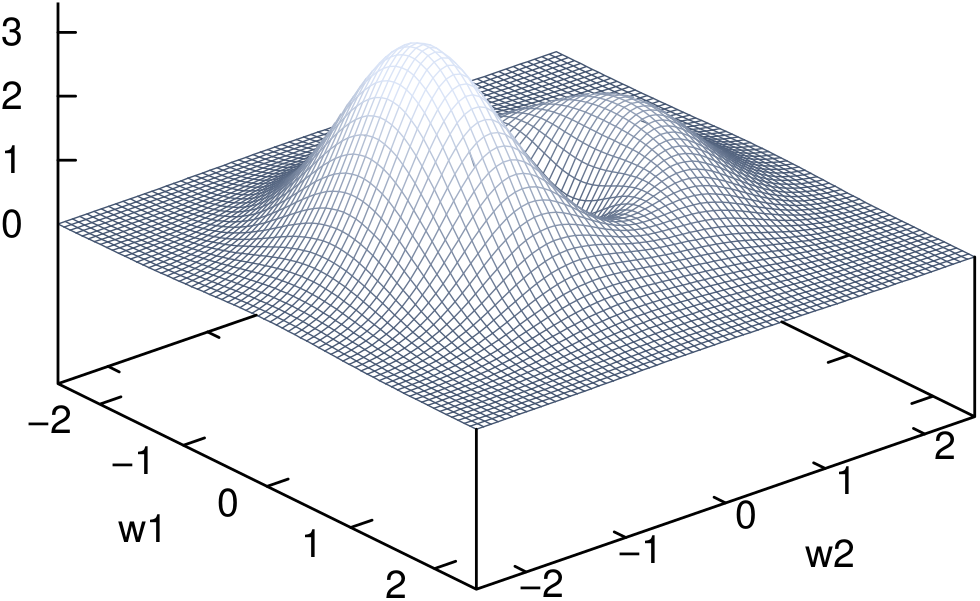
\includegraphics[width=0.5\textwidth]{Bilder/misc/Fehlerlandschaft.png}
    \caption{Beispiel einer Fehlerfläche eines Neuronalen Netzes mit zwei trainierbaren Gewichten. Bei weiteren Gewichten entsteht pro Gewicht eine zusätzliche Dimension in der Fehlerlandschaft. Was zu höherer Komplexität und zerklüfteter \glqq Oberfläche\grqq führt.\protect\footnotemark{}}
    \label{fig:Fehlerlandschaft}
\end{figure}
\addtocounter{footnote}{-1}     %  -1 mal die Gesamtanzahl an Fußnoten in der wrapfigure
\addtocounter{Hfootnote}{-1}    % -1 times total number of footnote(mark)s in the wrapfigure
\wrapfigfoot\footnotetext{\autoref{fig:Fehlerlandschaft} wurde aus \citet[80]{dkriesel07} übernommen.}

Durch anwendung des Gradientenabstigverfahrens\,\citef[63 f]{dkriesel07} kann nun vom Ausgangspunkt gesehen das nächste Minimum gefunden werden. Mit
\begin{equation}
\Delta w = - \alpha \nabla Err(W)
\end{equation}
erhält man nun die Information wie die Gewichte verändert werden können, um das Fehlerminimum zu finden.
Wobei $\alpha$ eine Proportionalitätskonstante darstellt, welche für die Schrittweite beim Gradientenabstieg verantwortlich ist.
Um zu erfahren wie jedes Gewicht verändert werden soll muss die Fehlerfunktion $Err(W)$ nach dem entsprechenden Gewicht $w_{ij}$ abgeleitet werden
\begin{equation}
\Delta w_{ij} = - \alpha \frac{\partial Err(W)}{\partial w_{ij}} .
\label{gl:gewaend}
\end{equation}

Die Fehlerfunktion $Err_p(W)$ für ein Trainingsbeispiel $p$ lässt sich auf unterschiedliche Weise bestimmen\,\footnote{\citet[60 f]{dkriesel07} gibt hierfür einige Beispiele an.}, an dieser Stelle wird der quadratische Abstand genutzt. Damit kann die Fehlerfunktion über alle Ausgabeneuronen berechnet werden mit:
\begin{equation}
Err_p(W)= \frac{1}{2} \sum^k_{j=1} (t_{pj}-o_{pj})^2 .
\end{equation}
Somit reduziert sich die Fehlerfunktion bei der Betrachtung eines Ausgabeneurons $j$ für ein Trainingsbeispiel $p$ zu
\begin{equation}
Err_p(W)= \frac{1}{2} (t_{pj}-o_{pj})^2 .
\label{gl:errp}
\end{equation}


Dabei entspricht bei dem Onlinelernen der Gesamtfehler $Err(W)$ dem Einzelfehler $Err_p(W)$
\begin{equation}
Err(W)=Err_p(W) 
\end{equation}
und bei dem Offlinelernen müssen die Einzelfehler aufsummiert werden
\begin{equation}
Err(W)= \sum^P_{p=1} Err_p(W). 
\end{equation}

Da in der \autoref{gl:errp} $t_{pj}$ konstant ist hängt $Err_p(W)$ nur von $o_{pj}$ ab. So kann die Ableitung $\frac{\partial Err_p(W)}{\partial w_{ij}}$ mit der Kettenregel zerlegt werden in
\begin{equation}
\frac{\partial Err_p(W)}{\partial w_{ij}}= \frac{\partial Err_p(W)}{\partial o_{pj}} \cdot \frac{\partial o_{pj}}{\partial w_{ij}}.
\label{gl:zerlket}
\end{equation}

Durch das Ableiten(\farbig{evtl. Differentitation}) der \autoref{gl:errp} nach $o_{pj}$ und einsetzen von \autoref{gl:delta} erhält man
\begin{equation}
\frac{\partial Err_p(W)}{\partial o_{pj}} = -(t_{pj}-o_{pj}) = - \delta_{pj} .
\label{gl:minusdelta}
\end{equation}

Unter Betrachtung der \autoref{gl:ausgang} kann der Ausdruck $ \frac{\partial o_{pj}}{\partial w_{ij}}$ nun auch geschrieben werden als 
\begin{equation}
\frac{\partial o_{pj}}{\partial w_{ij}} = \frac{\partial \sum\limits_{i=1}^n w_{ij} x_{pi}}{\partial w_{ij}} .
\label{gl:vor_xi}
\end{equation}
Wobei die abzuleitende Funktion zwar aus vielen Summanden zusammengesetzt ist aber nur der Summand $w_{ij} x_{pi}$ enthält die Variable $w_{ij}$ nach der abgeleitet wird. Es gilt also
\begin{equation}
\frac{\partial o_{pj}}{\partial w_{ij}} = x_{pi}.
\label{gl:xi}
\end{equation}
Durch das Einsetzen der \autoref{gl:xi} und \autoref{gl:minusdelta} in \autoref{gl:zerlket} erhält man:
\begin{equation}
\frac{\partial Err_p(W)}{\partial w_{ij}}= - \delta_{pj} \cdot x_{pi}.
\label{gl:ze}
\end{equation}
Somit kann mit der \autoref{gl:gewaend} die Deltaregel für das Onlinelernverfahren bestimmt werden:
\begin{equation}
\Delta w_{ij} = \alpha \cdot \delta_{pj} \cdot x_{pi} .
\label{gl:fertig_delta}
\end{equation}
Für das Offlinelernverfahren muss noch die Summe über alle Trainingsbeispiele gebildet werden
\begin{equation}
\Delta w_{ij} = \alpha \cdot \sum^P_{p=1} \delta_{pj} \cdot x_{pi} .
\end{equation}



%\subsection{Ergebnisse von \citet{Aggarwal2009} und \citet{Panapakidis2016}}\label{sec:andere_ergebnisse}

\todo{Liste der Märkte aus \citet{Cerjan2013}}

\todo{Tabellen einfügen und Hinweiß dass SVM keine ANN sind}

\subsection{Performancemaße}\label{sec:perfmas}
In diesem Abschnitt werden die Maße zur Evaluierung der Vorhersagegenauigkeit (weiterhin als Performancemaße bezeichnet) aufgeführt die in der Literaturrecherche zur Strompreismodellierung in \autoref{sec:strompreis} und weiterer Literatur\,\citef[5]{Guertler2017} genannt wurden. Hierbei $y_i$ und $\hat{y}_i$ die tatsächlichen und vorhergesagten Preise zum Zeitpunkt $i$ darstellen und $T$ die Gesamtanzahl der Zeitpunkte angibt. Außerdem gibt $\mean{y}$ den Mittelwert der tatsächlichen Preise und $\mean{y}_{train}$ den Preismittelwert der Trainingsdaten an.
%
Der Absolute Percentage Error (APE) liefert Informationen über die Fehlerverteilung in der Nähe der Null.\,\citef[14\label{foot:Domanski2017}]{Domanski2017}\farbig{reicht noch nicht}
%
% APE
\begin{equation}
APE= \sum\limits_{i \in T} \frac{\abs{y_i-\hat{y}_i}}{y_i}.
\label{gl:APE}
\end{equation}
%
%
Der Mean Absolute Percentage Error (MAPE) gibt einen prozentualen Mittelwert über den Fehlerbetrag an. Da das Ursprungsmaß (in dieser Arbeit als $MAPE_1$ bezeichnet) bei sehr kleinen Preisen einen hohen Werte liefert und bei einem Preis von Null sogar gegen Unendlich gehen wurden Mehrere Verbesserungen vorgeschlagen. Diese äußern sich durch einen Mittelwert über alle gemessenen Preise bei $MAPE_2$ oder durch einen Mittelwert aus der Betragssumme der des tatsächlichen und vorhergesagten Preises bei $sMAPE$ im Nenner. Hierbei steht ein Wert von 0\,\% für eine exakte und Werte um die 10\,\% für eine akkurate Vorhersage.\,\footnote{Vgl. \citet[17]{Bobinaite2016}, \citet[2105]{Amjady2009} und \citet[894]{Lago2018}.}   
% MAPE
\begin{equation}
MAPE_1= \frac{100}{T} \sum\limits_{i \in T} \frac{\abs{y_i-\hat{y}_i}}{y_i},
\label{gl:MAPE_1}
\end{equation}
%
% MAPE
\begin{equation}
MAPE_2= \frac{100}{T} \sum\limits_{i \in T} \frac{\abs{y_i-\hat{y}_i}}{\mean{y}},
\label{gl:MAPE_2}
\end{equation}
%
% sMAPE
\begin{equation}
sMAPE= \frac{100}{T} \sum\limits_{i \in T} \frac{\abs{y_i-\hat{y}_i}}{(\abs{y_i} + \abs{\hat{y}_i}) / 2}.
\label{gl:sMAPE}
\end{equation}
%
Der Mean Squared Error (MSE) gibt den quadratischen Mittelwert der der Fehler an und gibt an wie weit die vorhergesagten Daten von den tatsächlichen Werten liegen. Ein kleine Wert deutet auf eine gute vorhersage hin.\,\footnoteref{foot:Domanski2017}
% MSE
\begin{equation}
MSE= \frac{1}{T} \sum\limits_{i \in T} (y_i-\hat{y}_i)^2.
\label{gl:MSE}
\end{equation}
%
%
Der Root Mean Squared Error (RMSE) ist die Quadratwurzel des MSE und ist hierdurch sehr ähnlich. Der RMSE weist kleinere Werte auf, der Aussagegehalt ist aber ähnlich zu MSE.
% RMSE
\begin{equation}
RMSE= \sqrt{ \frac{1}{T} \sum\limits_{i \in T} (y_i-\hat{y}_i)^2}.
\label{gl:RMSE}
\end{equation}
%
Der Mean Absolut Error (MAE) ist ebenfalls sehr ähnlich zum MSE und damit auch dem RMSE. Weist aber im Vergleich zum RMSE nochmals kleinere Werte auf.
% MAE
\begin{equation}
MAE= \frac{1}{T} \sum\limits_{i \in T} \abs{y_i-\hat{y}_i}.
\label{gl:MAE}
\end{equation}
%
%
Der Normalized Mean Square Error (NMSE) ist ein Schätzwert über alle Abweichungen zwischen vorhergesagten und gemessenen Werten. Zeigt ein Modell einen sehr geringen NMSE so weist es eine gute örtliche und zeitliche Performance auf. Andererseits bedeuten hohe $NMSE$-Werte nicht, dass das betrachtete Modell komplett falsch ist.
% NMSE
\begin{gather}
\begin{aligned}
NMSE &= \frac{1}{\Delta^2 T} \sum\limits_{i \in T} (y_i-\hat{y}_i)^2,\\ 
\Delta^2 &= \frac{1}{T-1} \sum\limits_{i \in T} (y_i-\mean{y})^2.\\
\end{aligned}
\label{gl:NMSE}
\end{gather}
%
%
Die Error Variance (EV) gibt einen Wert über die nicht erklärten Informationen nach dem Fitten des Modells. Je kleiner der Wert ist desto präziser ist die Vorhersage.\,\citef{Peter2016}
% EV
\begin{equation}
EV= \sigma^2 = \frac{1}{T} \sum\limits_{i \in T} \left ( \frac{\abs{y_i-\hat{y}_i}}{\mean{y}} - MAPE_2  \right ) ^2.
\label{gl:EV}
\end{equation}
%
Pearson Korrelationskoeffizient bewertet die Linearität zwischen der Kovarianz zweier Variablen und dem Produkt der Standardabweichung dieser Variablen. Der Wertebereich dieses Maßes ist [-1,1] und er gibt Auskunft, wie Ähnlich der zeitliche Verlauf zwischen dem tatsächlichen Preis und der Vorhersage ist. Ein Wert von Eins deutet auf eine perfekte vorhersage hin.\,\citef{Davo2016} 
% cor
\begin{equation}
cor = \frac{cov(y_i,\hat{y}_i)}{\sqrt{sd(y_i)sd(\hat{y}_i)}} .
\label{gl:cor}
\end{equation}
%
%
Theils Koeffizienten der Ungleichheit U1 und U2 unterscheiden sich in der Anwesenheit bzw. Abwesenheit eines $\hat{y}_i$ im Nenner. Hierbei steht der Wert von Null in beiden fällen für Gleichheit und somit für eine ideale Vorhersage. Bei einem Wert von Eins spricht man von einer maximalen Ungleichheit. Dies kann bei U1 der Fall sein wenn eine negative Proportionalität besteht oder einer der Terme im Nenner Null ist. Bei dem U2 kann dies der Fall sein, wenn die Vorhersagemethode eine \textit{Na\"{i}ve-No-Change-Extrapolation}\,\citef[6]{Lattyak2011} ist oder wenn U2 zu der gleichen Standardabweichung des Prognosefehlers führt wie die Vorhersagemethode.\,\citef[444 f]{Bliemel1973}
% U1
\begin{equation}
U1 = \frac{\sqrt{\frac{1}{T} \sum_{i \in T} (y_i-\hat{y}_i)^2}}{ \sqrt{\frac{1}{T} \sum_{i \in T} y_i^2} + \sqrt{\frac{1}{T} \sum_{i \in T} \hat{y}_i^2}},
\label{gl:U1}
\end{equation}
%
% U2
\begin{equation}
U2 = \frac{\sqrt{\sum_{i \in T} (y_i-\hat{y}_i)^2}}{ \sqrt{ \sum_{i \in T} y_i^2} }.
\label{gl:U2}
\end{equation}
%
%
Das out-of-sample (R²) Bestimmtheitsmaß ist dem Relative Absolute Error (RAE) sehr ähnlich. Wenn das RAE kleiner 100 und das R² größer Null ist, so ist die Vorhersagegenauigkeit höher als der historische Mittelwert der Trainingsdaten.
% R²
\begin{equation}
R^2 = 1 -  \frac{\frac{1}{T} \sum_{i \in T} \abs{y_i-\hat{y}_i}^2}{ \frac{1}{T} \sum_{i \in T} \abs{y_i-\mean{y}_{train}}^2 } ,
\label{gl:R2}
\end{equation}
%
%
% RAE
\begin{equation}
RAE = \frac{\frac{1}{T} \sum_{i \in T} \abs{y_i-\hat{y}_i}}{ \frac{1}{T} \sum_{i \in T} \abs{y_i-\mean{y}_{train}} } \cdot 100 .
\label{gl:RAE}
\end{equation}
%
%
Der Absolute Error (ABS) und der Relative Error (REL) wertet den systematischen Fehler aus. Der Idealwert ist hierbei Null, wobei dies mit einer exakten Vorhersage gleichzusetzen ist. Positive Werte weisen dabei auf eine Überschätzung und negative auf eine Unterschätzung der Vorhersage hin.\,\citef[5 f]{Guertler2017}
%
% ABS
\begin{equation}
ABS= \frac{1}{T} \sum\limits_{i \in T} (\hat{y}_i-y_i),
\label{gl:ABS}
\end{equation}
%
%
% REL
\begin{equation}
REL= \frac{\sum_{i \in T} (\hat{y}_i-y_i)}{\sum_{i \in T} y_i} .
\label{gl:REL}
\end{equation}



%\begin{figure}[!htb]
%    \centering
%        
\pgfplotsset{every axis/.append style={
                label style={font=\footnotesize},
                tick label style={font=\footnotesize},
                x label style={yshift=.5em},
            }}
%%--------------------MAPE-MAE-RAE-------------------------%%
 \begin{tikzpicture}
 
    \def\datafile{Daten/BP/logist/m/BP_logis_m-epochen.dat}
 
    \pgfplotsset{
        %scale only axis,
        minor x tick num=1,
        xmin=0, xmax=51,
        width=15cm,
        height=8cm,
        ylabel style={rotate=180},
        xticklabel style={
            /pgf/number format/precision=3,
            /pgf/number format/fixed,
            x label style={yshift=.5em},
        },
    }
 
    \begin{axis}[
    axis y line*=left,
    xlabel=Epochen,
    ylabel=MAPE,
    y label style={yshift=.5em},
    %xlabel near ticks,
    minor y tick num=1,
    ]
    \addplot[
    mark=none,
    draw=green,
    ] 
    table[
    /pgf/number format/read comma as period,
    x=epochen, 
    y=MAPE_mean, 
    col sep=tab,
    ] {\datafile};
    \label{MAPE-}


       %\addplot[pattern=crosshatch,pattern color=blue!30!white,draw=blue!30!white]{x^2} \closedcycle;
       %\addplot[red,line legend] coordinates {(0,0) (1,1)};
       %\legend{RMSE,U2}
    \end{axis}

    \begin{axis}[
    axis x line=none,
    axis y line*=left,
    ylabel=MAE,
    y label style={yshift=.5em},
    minor y tick num=1,
    ] 
    %\addlegendimage{/pgfplots/refstyle=MAPE}\addlegendentry{MAPE}
    \pgfplotsset{
        every outer y axis line/.style={xshift=-1.2cm}, 
        every tick/.style={xshift=-1.2cm}, 
        every y tick label/.style={xshift=-1.2cm} 
    }
    
    \addplot[
    mark=none,
    draw=purple,
    ] 
    table[
    /pgf/number format/read comma as period,
    x=epochen, 
    y=MAE_mean,
    col sep=tab,
    ] {\datafile};
    \label{MAE-}
    \end{axis}
    
    \begin{axis}[
    axis x line=none,
    axis y line*=right,
    ylabel=RAE,
    y label style={yshift=-.5em},
    minor y tick num=1,
    ] 
    \addlegendimage{/pgfplots/refstyle=MAPE-}\addlegendentry{MAPE}
    \addlegendimage{/pgfplots/refstyle=MAE-}\addlegendentry{MAE}

    \addplot[
    mark=none,
    draw=cyan,
    ] 
    table[
    /pgf/number format/read comma as period,
    x=epochen, 
    y=RAE_mean, 
    col sep=tab,
    ] {\datafile};
    \addlegendentry{RAE}
    \end{axis}

   \end{tikzpicture}
%    \caption{Gegenüberstellung des $MAPE$, des $MAE$ und des $RAE$ wobei auffällt, dass die Maße sich in einem Faktor unterscheiden.}
%    \label{fig:geg_mape_mae_rae}
%\end{figure}

%\begin{figure}[!htb]
%    \centering
%        \pgfplotsset{every axis/.append style={
                label style={font=\footnotesize},
                tick label style={font=\footnotesize},
                x label style={yshift=.5em},
            }}

%%--------------------RMSE-U2----------------------------%%
 \begin{tikzpicture}
 
    \def\datafile{Daten/BP/logist/m/BP_logis_m-epochen.dat}
 
    \pgfplotsset{
        %scale only axis,
        minor x tick num=1,
        xmin=0, xmax=51,
        width=15cm, %\textwidth,
        height=8cm,
        ylabel style={rotate=180},
        xticklabel style={
            /pgf/number format/precision=3,
            /pgf/number format/fixed,
        },
    }
 
    \begin{axis}[
    axis y line*=left,
    xlabel=Epochen,
    ylabel=RMSE,
    y label style={yshift=.5em},
    %xlabel near ticks,
    minor y tick num=1,
    ]
    \addplot[
    mark=none,
    draw=black,
    ] 
    table[
    /pgf/number format/read comma as period,
    x=epochen, 
    y=RMSE_mean, 
    col sep=tab,
    ] {\datafile};
    \label{RMSE-}

    \end{axis}

    \begin{axis}[
    axis x line=none,
    axis y line*=right,
    ylabel=U2,
    y label style={yshift=-.5em},
    minor y tick num=1,
    ] 
    \addlegendimage{/pgfplots/refstyle=RMSE-}\addlegendentry{RMSE}
    %\pgfplotsset{
    %    every outer y axis line/.style={xshift=-1.2cm}, 
    %    every tick/.style={xshift=-1.2cm}, 
    %    every y tick label/.style={xshift=-1.2cm} 
    %}
    
    \addplot[
    mark=none,
    draw=red,
    ] 
    table[
    /pgf/number format/read comma as period,
    x=epochen, 
    y=U2_mean, 
    col sep=tab,
    ] {\datafile};
    \addlegendentry{U2}
    \end{axis}

   \end{tikzpicture}
%    \caption{Die gleiche Beobachtung wie in \autoref{fig:geg_mape_mae_rae} kann auch bei der Gegenüberstellung des $RMSE$ und des $U2$ gemacht werden.}
%    \label{fig:geg_rmse_u2}
%\end{figure}

%\begin{landscape}
%\begin{figure}[!htb]
%    \centering
%        \pgfplotsset{every axis/.append style={
                label style={font=\footnotesize},
                tick label style={font=\footnotesize},
                x label style={yshift=.5em},
            }}
%%--------------------alle-------------------------%%
 \begin{tikzpicture}
 
    \def\datafile{Daten/BP/logist/m/BP_logis_m-epochen.dat}

    \def\xshiftlab{1.1cm}
 
    \pgfplotsset{}
 
    \pgfplotsset{
        %scale only axis,
        minor x tick num=1,
        xmin=0, xmax=51,
        width=15cm, %\textwidth,
        height=13cm,
        ylabel style={rotate=180},
        xticklabel style={
            /pgf/number format/precision=3,
            /pgf/number format/fixed},
        every axis legend/.append style={
        at={(0.5,1.03)},
        anchor=south},
    }
 %%----------------------RMSE-----------------------------%%
    \begin{axis}[
    axis y line*=left,
    xlabel=Epochen,
    ylabel=RMSE,
    y label style={yshift=.5em},
    xlabel near ticks,
    minor y tick num=1,
    ]
    \addplot[
    mark=none,
    draw=black,
    ] 
    table[
    /pgf/number format/read comma as period,
    x=epochen, 
    y=RMSE_mean, 
    col sep=tab,
    ] {\datafile};
    \label{RMSE}
    \end{axis}

%%------------------------U2------------------------------%%
    \begin{axis}[
    axis x line=none,
    axis y line*=left,
    ylabel=U2,
    y label style={yshift=.75em},
    minor y tick num=1,
    ] 
    \pgfplotsset{
        every outer y axis line/.style={xshift=-\xshiftlab*1.2}, 
        every tick/.style={xshift=-\xshiftlab*1.2}, 
        every y tick label/.style={xshift=-\xshiftlab*1.2} 
    }
    
    \addplot[
    mark=none,
    draw=red,
    ] 
    table[
    /pgf/number format/read comma as period,
    x=epochen, 
    y=U2_mean, 
    col sep=tab,
    ] {\datafile};
    \label{U2}
    \end{axis}

%%------------------------REL------------------------------%%
    \begin{axis}[
    axis x line=none,
    axis y line*=left,
    ylabel=REL,
    y label style={yshift=.6em},
    minor y tick num=1,
    ] 
    \pgfplotsset{
        every outer y axis line/.style={xshift=-\xshiftlab*2.3}, 
        every tick/.style={xshift=-\xshiftlab*2.3}, 
        every y tick label/.style={xshift=-\xshiftlab*2.3} 
    }
    
    \addplot[
    mark=none,
    draw=orange,
    ] 
    table[
    /pgf/number format/read comma as period,
    x=epochen, 
    y=REL_mean, 
    col sep=tab,
    ] {\datafile};
    \label{REL}
    \end{axis}

%%------------------------ABS------------------------------%%
    \begin{axis}[
    axis x line=none,
    axis y line*=left,
    ylabel=ABS,
    y label style={yshift=.6em},
    minor y tick num=1,
    ] 
    \pgfplotsset{
        every outer y axis line/.style={xshift=-\xshiftlab*3.45}, 
        every tick/.style={xshift=-\xshiftlab*3.45}, 
        every y tick label/.style={xshift=-\xshiftlab*3.45} 
    }
    
    \addplot[
    mark=none,
    draw=lime,
    ] 
    table[
    /pgf/number format/read comma as period,
    x=epochen, 
    y=ABS_mean, 
    col sep=tab,
    ] {\datafile};
    \label{ABS}
    \end{axis}

%%------------------------EV------------------------------%%
    \begin{axis}[
    axis x line=none,
    axis y line*=left,
    ylabel=EV,
    y label style={yshift=.5em},
    minor y tick num=1,
    ] 
    \pgfplotsset{
        every outer y axis line/.style={xshift=-\xshiftlab*4.45}, 
        every tick/.style={xshift=-\xshiftlab*4.45}, 
        every y tick label/.style={xshift=-\xshiftlab*4.45} 
    }
    
    \addplot[
    mark=none,
    draw=brown,
    ] 
    table[
    /pgf/number format/read comma as period,
    x=epochen, 
    y=EV_mean, 
    col sep=tab,
    ] {\datafile};
    \label{EV}
    \end{axis}





%%----------------------sMAPE-----------------------------%%
    \begin{axis}[
    axis x line=none,
    axis y line*=right,
    %xlabel=Epochen,
    ylabel=sMAPE,
    y label style={yshift=-.5em},
    minor y tick num=1,
    ]
    \addplot[
    mark=none,
    draw=magenta,
    ] 
    table[
    /pgf/number format/read comma as period,
    x=epochen, 
    y=sMAPE_mean, 
    col sep=tab,
    ] {\datafile};
    \label{sMAPE}
    \end{axis}

%%----------------------MAPE-----------------------------%%
    \begin{axis}[
    axis x line=none,
    axis y line*=right,
    %xlabel=Epochen,
    ylabel=MAPE,
    y label style={yshift=-.5em},
    minor y tick num=1,
    ]
    
    \pgfplotsset{
        every outer y axis line/.style={xshift=\xshiftlab}, 
        every tick/.style={xshift=\xshiftlab}, 
        every y tick label/.style={xshift=\xshiftlab} 
    }
    
    \addplot[
    mark=none,
    draw=green,
    ] 
    table[
    /pgf/number format/read comma as period,
    x=epochen, 
    y=MAPE_mean, 
    col sep=tab,
    ] {\datafile};
    \label{MAPE}
    \end{axis}

%%----------------------MAE-----------------------------%%
    \begin{axis}[
    axis x line=none,
    axis y line*=right,
    ylabel=MAE,
    y label style={yshift=-.85em},
    minor y tick num=1,
    ] 
    %\addlegendimage{/pgfplots/refstyle=MAPE}\addlegendentry{MAPE}
    \pgfplotsset{
        every outer y axis line/.style={xshift=\xshiftlab*2}, 
        every tick/.style={xshift=\xshiftlab*2}, 
        every y tick label/.style={xshift=\xshiftlab*2} 
    }
    
    \addplot[
    mark=none,
    draw=purple,
    ] 
    table[
    /pgf/number format/read comma as period,
    x=epochen, 
    y=MAE_mean,
    col sep=tab,
    ] {\datafile};
    \label{MAE}
    \end{axis}

%%----------------------RAE-----------------------------%%
    \begin{axis}[
    axis x line=none,
    axis y line*=right,
    ylabel=RAE,
    y label style={yshift=-.5em},
    minor y tick num=1,
    ]

    \pgfplotsset{
        every outer y axis line/.style={xshift=\xshiftlab*3}, 
        every tick/.style={xshift=\xshiftlab*3}, 
        every y tick label/.style={xshift=\xshiftlab*3} 
    }

    \addplot[
    mark=none,
    draw=cyan,
    ] 
    table[
    /pgf/number format/read comma as period,
    x=epochen, 
    y=RAE_mean, 
    col sep=tab,
    ] {\datafile};
    \label{RAE}
    \end{axis}

%%----------------------R²-----------------------------%%
    \begin{axis}[
    axis x line=none,
    axis y line*=right,
    ylabel=R$^2$,
    y dir=reverse,
    y label style={yshift=-.5em},
    minor y tick num=1,
    legend columns=10,
    ]
    
    \addlegendimage{/pgfplots/refstyle=RMSE}\addlegendentry{RMSE}
    \addlegendimage{/pgfplots/refstyle=U2}\addlegendentry{U2}
    \addlegendimage{/pgfplots/refstyle=REL}\addlegendentry{REL}
    \addlegendimage{/pgfplots/refstyle=ABS}\addlegendentry{ABS}
    \addlegendimage{/pgfplots/refstyle=EV}\addlegendentry{EV}
    \addlegendimage{/pgfplots/refstyle=sMAPE}\addlegendentry{sMAPE}
    \addlegendimage{/pgfplots/refstyle=MAPE}\addlegendentry{MAPE}
    \addlegendimage{/pgfplots/refstyle=MAE}\addlegendentry{MAE}
    \addlegendimage{/pgfplots/refstyle=RAE}\addlegendentry{RAE}

    \pgfplotsset{
        every outer y axis line/.style={xshift=\xshiftlab*4}, 
        every tick/.style={xshift=\xshiftlab*4}, 
        every y tick label/.style={xshift=\xshiftlab*4} 
    }

    \addplot[
    mark=none,
    draw=blue,
    ] 
    table[
    /pgf/number format/read comma as period,
    x=epochen, 
    y=R2_mean, 
    col sep=tab,
    ] {\datafile};
    \addlegendentry{R2}
    \end{axis}

   \end{tikzpicture}
%    \caption{Dargestellt ist die Messung der optimalen Epochenanzahl eines MLPs mit Bias-Neuron welches mit dem BP-Verfahren trainiert wird und eine logistische Aktivierungsfunktion besitzt. Dieser Graph dient der Gegenüberstellung aller in dieser Arbeit betrachteten Performancemaße.}
%    \label{fig:geg_alle}
%\end{figure}
%\end{landscape}

%-----------------------------------------------------------------------------------
\todo{Fehlermaße aufführen und bedeutung erkären}


%---------------------------------------------------------------------------------
\newpage
%---------------------------------------------------------------------------------
%% Schluss

\pagenumbering{Roman}

\section{Literaturverzeichnis}

\printbibliography


%\bibliographystyle{alpha}               % Stil des Literaturverzeichnisses 
%\bibliography{10_literatur}             % Aufruf des Literaturverzeichnisses






%-------------
%% Einstellungen für die richtige Darstellung von Fußnoten und Hyperlinks
\AtEndDocument{%
\ifnum\value{Hfootnote}=\value{footnote}%OK
  \PackageInfo{footnote}{%
    Number of Hyperfootnotes \arabic{Hfootnote} = number of footnotes \arabic{footnote}!
    \MessageBreak%
    }
\else
  \PackageError{footnote}{%
    Hyperfootnote \arabic{Hfootnote} != footnote \arabic{footnote}!%
   }{Did you make a mistake with\MessageBreak%
     \string\footnotemark , \string\footnotetext , or \MessageBreak%
     \string\addtocounter { Hfootnote or footnote } ?%
   }
\fi%
%\thispagestyle{empty}    
}
%-------------
\end{document}